\documentclass[12pt,a4paper]{report}

% third part package
\usepackage[latin1]{inputenc}
\usepackage{amsmath}
\usepackage{amsfonts}
\usepackage{amssymb}
\usepackage{fullpage}
\usepackage{titlepic}
\usepackage{graphicx}
\usepackage{float}
\usepackage{fancyhdr}
\usepackage[headsep=1cm,headheight=2cm, margin=0.7in]{geometry} 
\usepackage{hyperref}
\hypersetup{
	colorlinks,
	citecolor=black,
	filecolor=black,
	linkcolor=black,
	urlcolor=black
}
\usepackage{apacite}

% title information
\titlepic{
\includegraphics[width=12em]{./pics/Dog-Icon-letter.png}}
\title{GitGroup - A Web Based Software Development Management System}
\date{\today}
\author{Runbo ZHAO \\ Jingyu BAO \\ Xuying CAO \\ Chengxiang YIN
\\[1cm]{\small Advisor: Edmund S. Yu} \\ {\small Course: CSE 682 Software Engineering}}

\begin{document}
\pagenumbering{gobble}

% title and table of contents page
\maketitle
\tableofcontents
\newpage

% start paging
\cleardoublepage
\pagenumbering{arabic}
\pagestyle{fancy}

% ----------------------------------------------------
% Chapter 1 Introduction
% ----------------------------------------------------

\chapter{Introduction}
\section{Purpose}
The document is an official statement of what the system developers should implement. It includes both the user requirements for a system and a detailed specification of the system requirements. The document is essential for outside contractor who developing the software system. It is also useful to write a short supporting document that defines the business and dependability requirement for the system. The document is for system customers, managers, system engineers, system test engineers, system maintenance engineers.
\section{What are GitHub APPs?}
GitHub Apps are first-class actors within GitHub. A GitHub App acts on its own behalf, taking actions via the API directly using its own identity, which means you don't need to maintain a bot or service account as a separate user.\\
GitHub Apps can be installed directly on organizations and user accounts and granted access to specific repositories. They come with built-in webhooks and narrow, specific permissions. When you set up for your GitHub App, you can select the repositories you want it to access.\\
Some key ideas when creating GitHub Apps
\begin{enumerate}
	\renewcommand{\labelenumi}{{\textbf{\arabic{enumi}.}}}
	\item A GitHub App should take actions independent of a user (unless the app is using a user-to-server token).
	\item Make sure the GitHub App integrates with specific repositories.
	\item The GitHub App should connect to a personal account or an organization.
	\item Don't expect the GitHub App to know and do everything a user can.
	\item Don't use a GitHub App if you just need a "Login with GitHub" service. But a GitHub App can use a user identification flow to log users in and do other things.
	\item Don't build a GitHub App if you only want to act as a GitHub user and do everything that user can do.
\end{enumerate}
GitHub Marketplace contains tools and services that complement and improve workflow. Anyone can discover, browse, and install free and paid GitHub App and OAuth Apps in GitHub Marketplace.
\begin{figure}[H]
	\centering
	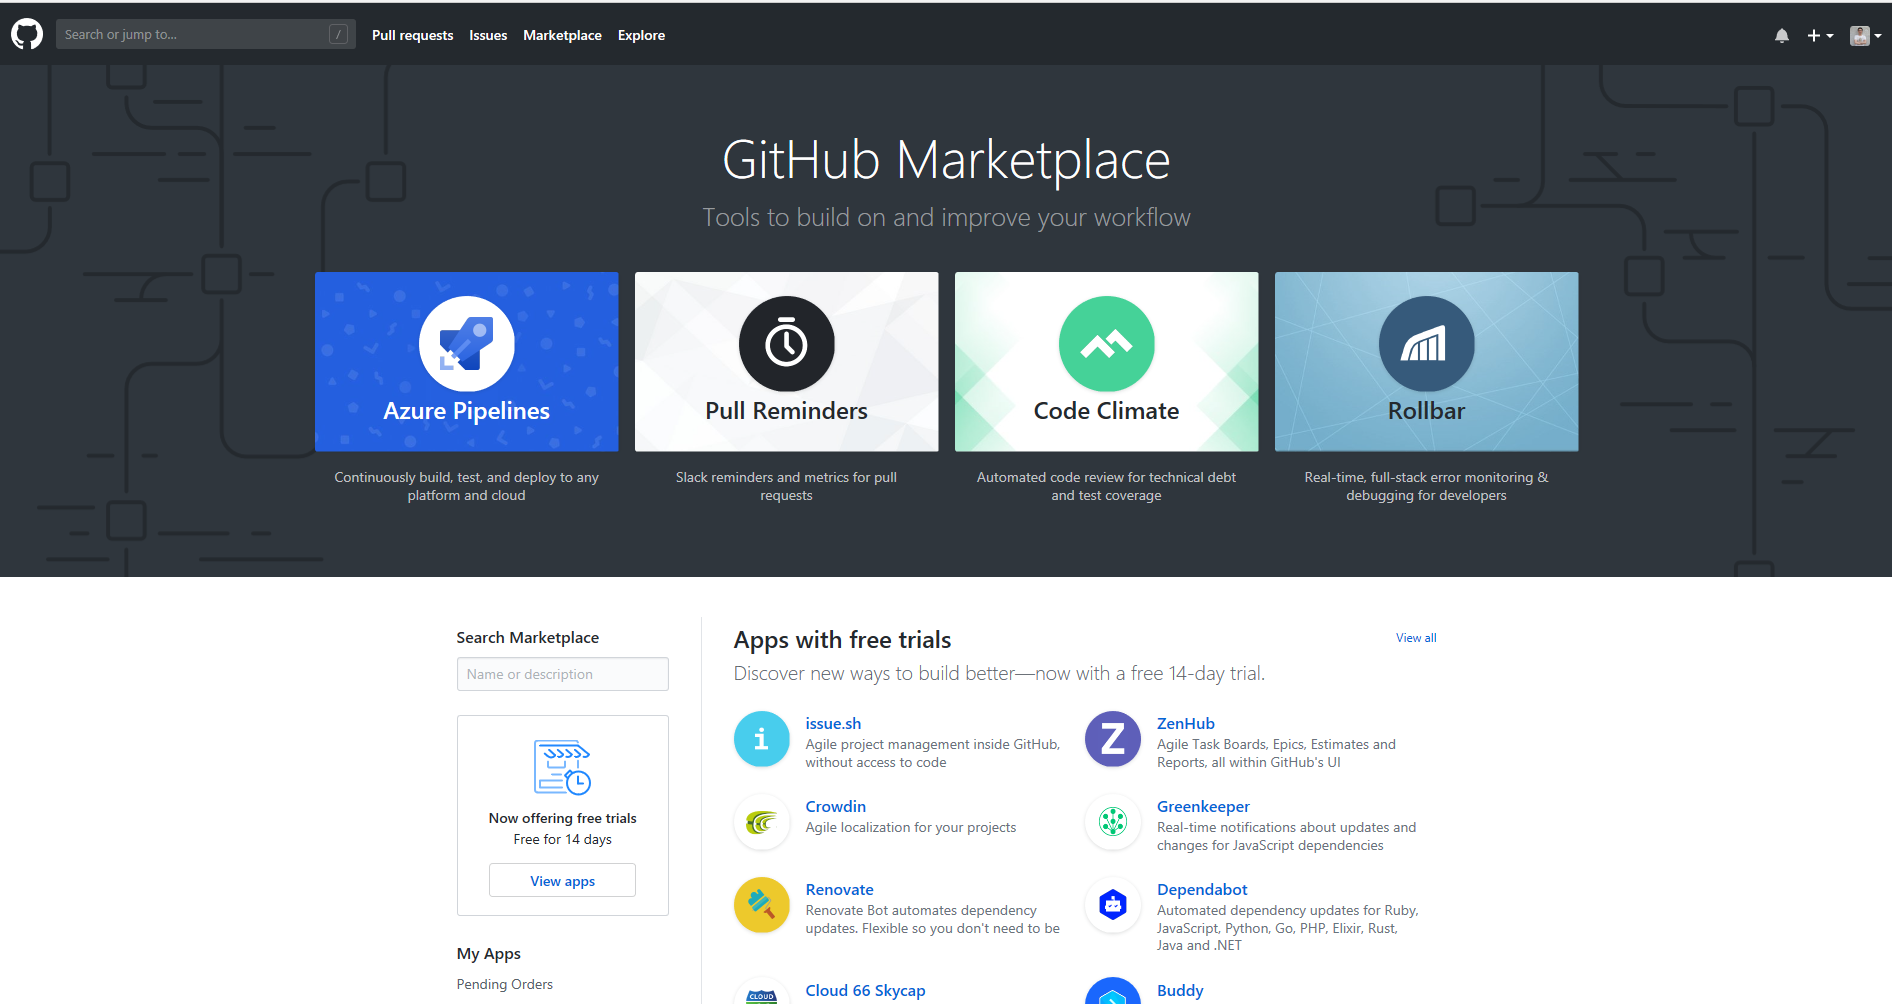
\includegraphics[width=0.8\textwidth]{./pics/githubMarket.png}
	\caption{GitHub Marketplace}
\end{figure}
The following is the home page of GitGroup in GitHub.
\begin{figure}[H]
	\centering
	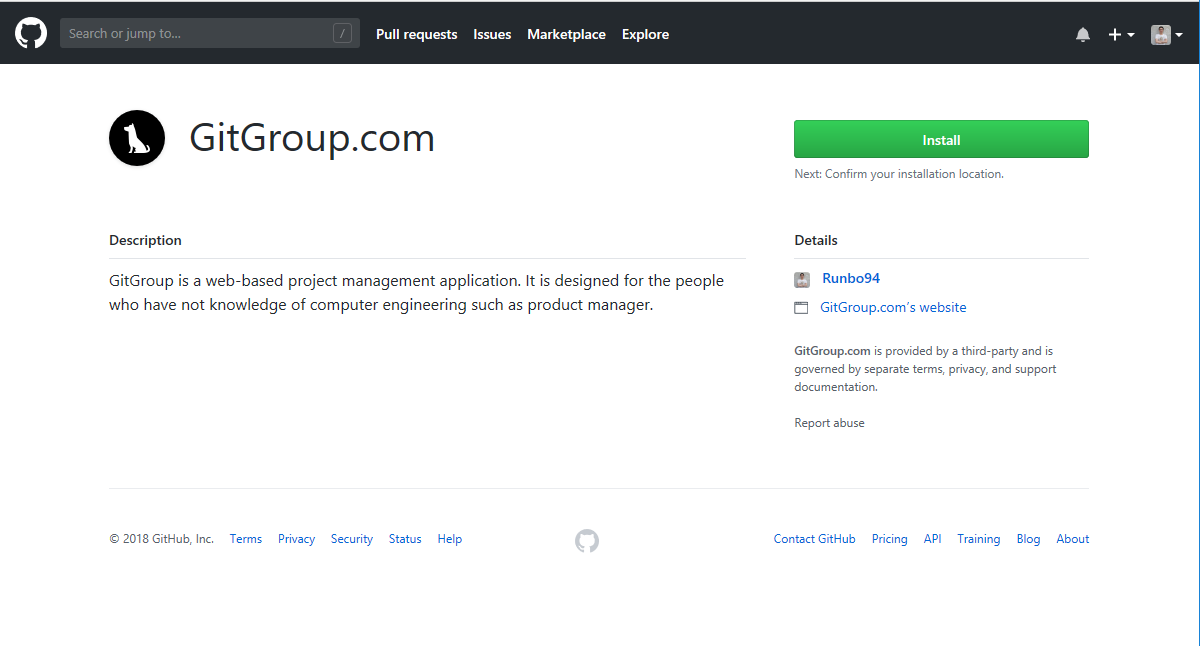
\includegraphics[width=0.8\textwidth]{./pics/gitgrouphomepage.png}
	\caption{GitHub Marketplace}
\end{figure}
\section{Product Scope}
GitGroup is a web-based GitHub Application. It is a project management platform that allows everyone on your team to communicate with the developers. Therefore, GitGroup is not only designed for programmer but also for people who has less development experience such as project manager, project members and people who are related to the project. On GitGroup, it is easy to create an Agile workflow for your team with a kanban board. GitGroup?s seamless integration with GitHub keeps all of your GitHub Issue data in sync across both platforms in real time.
It is an easy access web-based application that served for product management team based on Github API.\\
GitGroup is built by several software development tools. From the perspective of programming language, we use both TypeScript and JavaScript. TypeScript is an open-source programming language.It is a strict syntactical superset of JavaScript, and adds optional static typing to the language. And its strong Object-Oriented Programming features make it as a best developing language for building GitGroup. When the developing is done, TypeScript compiler can compile the source code to JavaScript program in order to let it run on the NodeJS. Javascript is a language which is also characterized as dynamic, weakly typed, prototype-based and multi-paradigm.\\
From the perspective of framework. ReactJS(Front end framework), Bulma(CSS framework), Frontawesome(Icon set and toolkit), ExpressJS(Back end framework) is chose. In the test process, our tool is Jest. It is a Javascript testing software. Jest is used by Facebook to test all JavaScript code including React applications. One of Jest's philosophies is to provide an integrated "zero-configuration" experience. This feature of Jest make the duration of developing shorter. Also we regard MongoDB as our host DBMS, which is one of the most popular database management tool. Other tools such as Git, Heroku, Visual Studio Code, Postman, are also included in developing process.\\

\section[Def., Acronyms and Abbr.]{Definitions, Acronyms and Abbreviations}
\begin{table}[H]
	\centering
	\begin{tabular}{|l|l|}
		\hline
		Git        & A version-control system for tracking changes in computer files                                                                \\ \hline
		GitHub     & A web-based hosting service for version control using Git                                                               \\ \hline
		REST     & The architectural style defines constraints used for creating web services.                                                          \\ \hline
		Owner        & Who set up the project or mainly charge of the project \\ \hline
		Collaborator & Who assists owner or project participants              \\ \hline
		Project      & An element in GitGroup, including multiple repository  \\ \hline
		Repository   & A folder which contains all project's files and stores each file's revision history                                                       		  \\
		\hline
		Issue        & Information used to track ideas, enhancements, tasks, or bugs on GitHub                                                               \\ 
		\hline
		KanBan       & A scheduling system for lean and just-in-time manufacturing                                                         \\ \hline
		Cards        & A message that signals depletion of product, parts, or inventory on KanBan                                                                \\ \hline
	\end{tabular}
	\caption{Definitions, Acronyms and Abbreviations}
\end{table}
\section{Overview of The Document}
The rest of the document will include overall description of Gitgroup in following perspectives. Product perspective, product functions, user characteristics, operating environment, design and implementation constraints, assumptions and dependencies. For interface requirement, we put efforts on user interfaces, hardware interfaces, software interfaces and communications interfaces. we will also include requirements like user requirements, system requirements, functional requirements, non-functional requirements and system models like use case diagram, activity diagram, sequence diagram, class diagram, system architecture, web design. 

% ----------------------------------------------------------
% Chapter 2 Overall Description
% ----------------------------------------------------------
\chapter{Overall Description}
This section of the SRS will include general factors that affect the product and its requirements. This section does not state specific requirements. Instead, it provides a background for those requirements, which are defined in detail in Section 3 of the SRS, and makes them easier to understand. 
\section{Product Perspective}
The background of the Gitgroup coming from project managers are often busy to managing multiple projects at the same time. Sometimes, they are not familiar with details with products especially in technology perspective. However, Git and Github have a high entrance standard which project manager hard to manipulate it. For example, when you want to create an issue to suggest a new idea or track a bug, you need to learn markdown syntax, emoji code. And it is even more complex when you do pull request and merge the project. Comparing with Git and Github,   GitGroup is an easier access tool . People who has little development experience, such as product manager. They also can handle GitGroup easily. The only thing they need to do is sign up an account and access to the GitHub api. The user can create online group chat, schedual and resord conference. After finding project idea, our online app also provide the task management service. In each project, every user will have their own grade. Furthermore, the online web can have a recommendation system which help the product manager and programmer match each other. In conclusion, it is a online service based on the GitHub API, and improve the user experience. 
\section{Product Functions}
Our product focus on easy access, clearly, convenience, efficiency. Fuctions are surrounded our goals. Mainly function lists in the following.
\begin{enumerate}
	\renewcommand{\labelenumi}{{\textbf{\arabic{enumi}.}}}

	\item KanBan:
	The Kanban board which is similar to projects board in the Gitub. In the Kanban board, there are several columns represent different stage of the developement process. You can customize your own stage. Every column contains issue card imported from the Github, and you can easily drug them among the columns. If you drug it to the Done column. The issue in the Github will be automatically closed.
	\item Chart - Project Analytics: 
	GitGroup offers a variety of Agile charts and analytics to help you keep track of how your team is doing. 
	\item Online Meeting and Chatting: 
	Online meeting group chat. Record the conference. Make conference scheduling form and alarming the coming meeting. GitGroup offers chat room for users to communication. There are two types of chat. One is global chat which is used to communicate friends directly. Another is in-team chat which is used to communicate among the team members. for you.
\end{enumerate}

\section{User Characteristic}
First of all, every use can create their own projects. If they are in their own projects, they are owners, verse and vice, they are collaborator. Therefore, one user can be both owner and collaborator according the project they are managing.\\
After entering a project, GitGroup will consist of 2 user flows, one for the owner of project, and the other for the collaborator. A high-level summary of the most important features offered by the system with respect to each of these users are as follows, 
	\subsection{For Every User}
	\begin{enumerate}
	\renewcommand{\labelenumi}{{\textbf{\arabic{enumi}.}}}
	\item Every user can create their own project.
	\item Every user can use global chat to communicate all your friends directly.
	\item Every user can get notification from system or other users.
	\item Every user can view and edit their own personal profile.
\end{enumerate}	 
	\subsection{For Collaborator}
	\begin{enumerate}
		\renewcommand{\labelenumi}{{\textbf{\arabic{enumi}.}}}
		\item The collaborator can enter the KanBan board. In the KanBan board, they can add cards, drug and move current cards, edit the content of cards.
		\item The collaborator can view the analytics which is different types of charts. to help keep track of how your team is doing.
		\item The collaborator can use in-team chat to communicate with other developers in the team.
	\end{enumerate}
	\subsection{For Owner}
	\begin{enumerate}
		\renewcommand{\labelenumi}{{\textbf{\arabic{enumi}.}}}
		\item The owner can do anything the collaborators can do.
		\item The owner can invite other user to your project as collaborator.
		\item The owner can remove any collaborators in your project.
		\item The owner can add any your GitHub repositories to your project.
		\item The owner can remove any GitHub repositories in your project.
		\item The owner can add new KanBans in your KanBan board.
		\item The owner can remove any KanBans in your KanBan board.
		\item The owner can add new columns to any Kanbans and remove add columns in Kanban.
	\end{enumerate}
\section{Operating Environment}
The system will implement the model-view-controller software architecture pattern. The operating environment for the system consists of a browser that renders web pages, an external web server that handles user request-response transactions, an authentication and authorization server as well as a database for storing application data. Servers with reasonable load handling capacity will be sufficient for web hosting and data storage. Central administration is vested in the web/application server. 
\section{Design And Implementation Constraints}
\begin{enumerate}
	\renewcommand{\labelenumi}{{\textbf{\arabic{enumi}.}}}
	\item The key constraints of the system is the inherent reliability on an internet connection. Since the product is implemented using the client-server model, it is imperative to have an active internet connection.  
	\item Because GitGroup is deployed on Heroku. There are some constraints from Heroku including the application will sleep after 30 mins of inactivity, monthly pool of 1000 Free dyno hours. When a Free dyno is active, it draws from the pool; the application can run as long as there are dyno hours left in your monthly pool.
	\item Because GitGroup will use GitHub API, the constraints come from the status of the GitHub API.
\end{enumerate}
\section{Assumptions And Dependencies}
	\subsection{Assumptions}
	\begin{enumerate}
		\renewcommand{\labelenumi}{{\textbf{\arabic{enumi}.}}}
		\item Since the system will be deployed using a cloud based hosting service, an assumption about its continuous, uninterrupted availability is made.   
		\item The system will depend on a trusted third party financial institution for handling monetary transactions. Hence, an assumption about total financial security is made. 
	\end{enumerate}
	\subsection{Dependencies}
		\begin{enumerate}
		\renewcommand{\labelenumi}{{\textbf{\arabic{enumi}.}}}
		\item The system will rely heavily on frameworks for user interface development, routing and data handling.   
		\item The system depends on the Heroku deployment platform.
		\item The system depends on mLab Cloud Database.
		\item The system will rely on some third part package, all the dependencies information is in the package.json file in the TypeScript and JavaScript projet.
	\end{enumerate}

% -----------------------------------------------------
% Chapter 3 Interface Requirement
% -----------------------------------------------------
\chapter{Interface Requirements}
\section{User Interfaces}
Thu style of GitGroup UI must be clean and easy to use. The CSS framework GitGroup choose is Bulma. It is a beautiful, lightweight and stylish CSS framework. and its grid is fully built with flexbox. Achieving flexible layout with same-size columns is as simple as adding \textbf{.column} class to HTML element. Furthermore, Bulma has some GitHub design style component like panel. It can be easy reuse to build GitGroup project lists.\\
The icon set and toolkits chose for GitGroup is Font Awesome. Font Awesome is a font and icon toolkit based on CSS and LESS. It was made by Dave Gandy for use with Twitter Bootstrap, and later was incorporated into the BootstrapCDN. Font Awesome has a 20% market share among those websites which use third-party Font Scripts on their platform, ranking it second place after Google Fonts.
\begin{figure}[H]
	\centering
	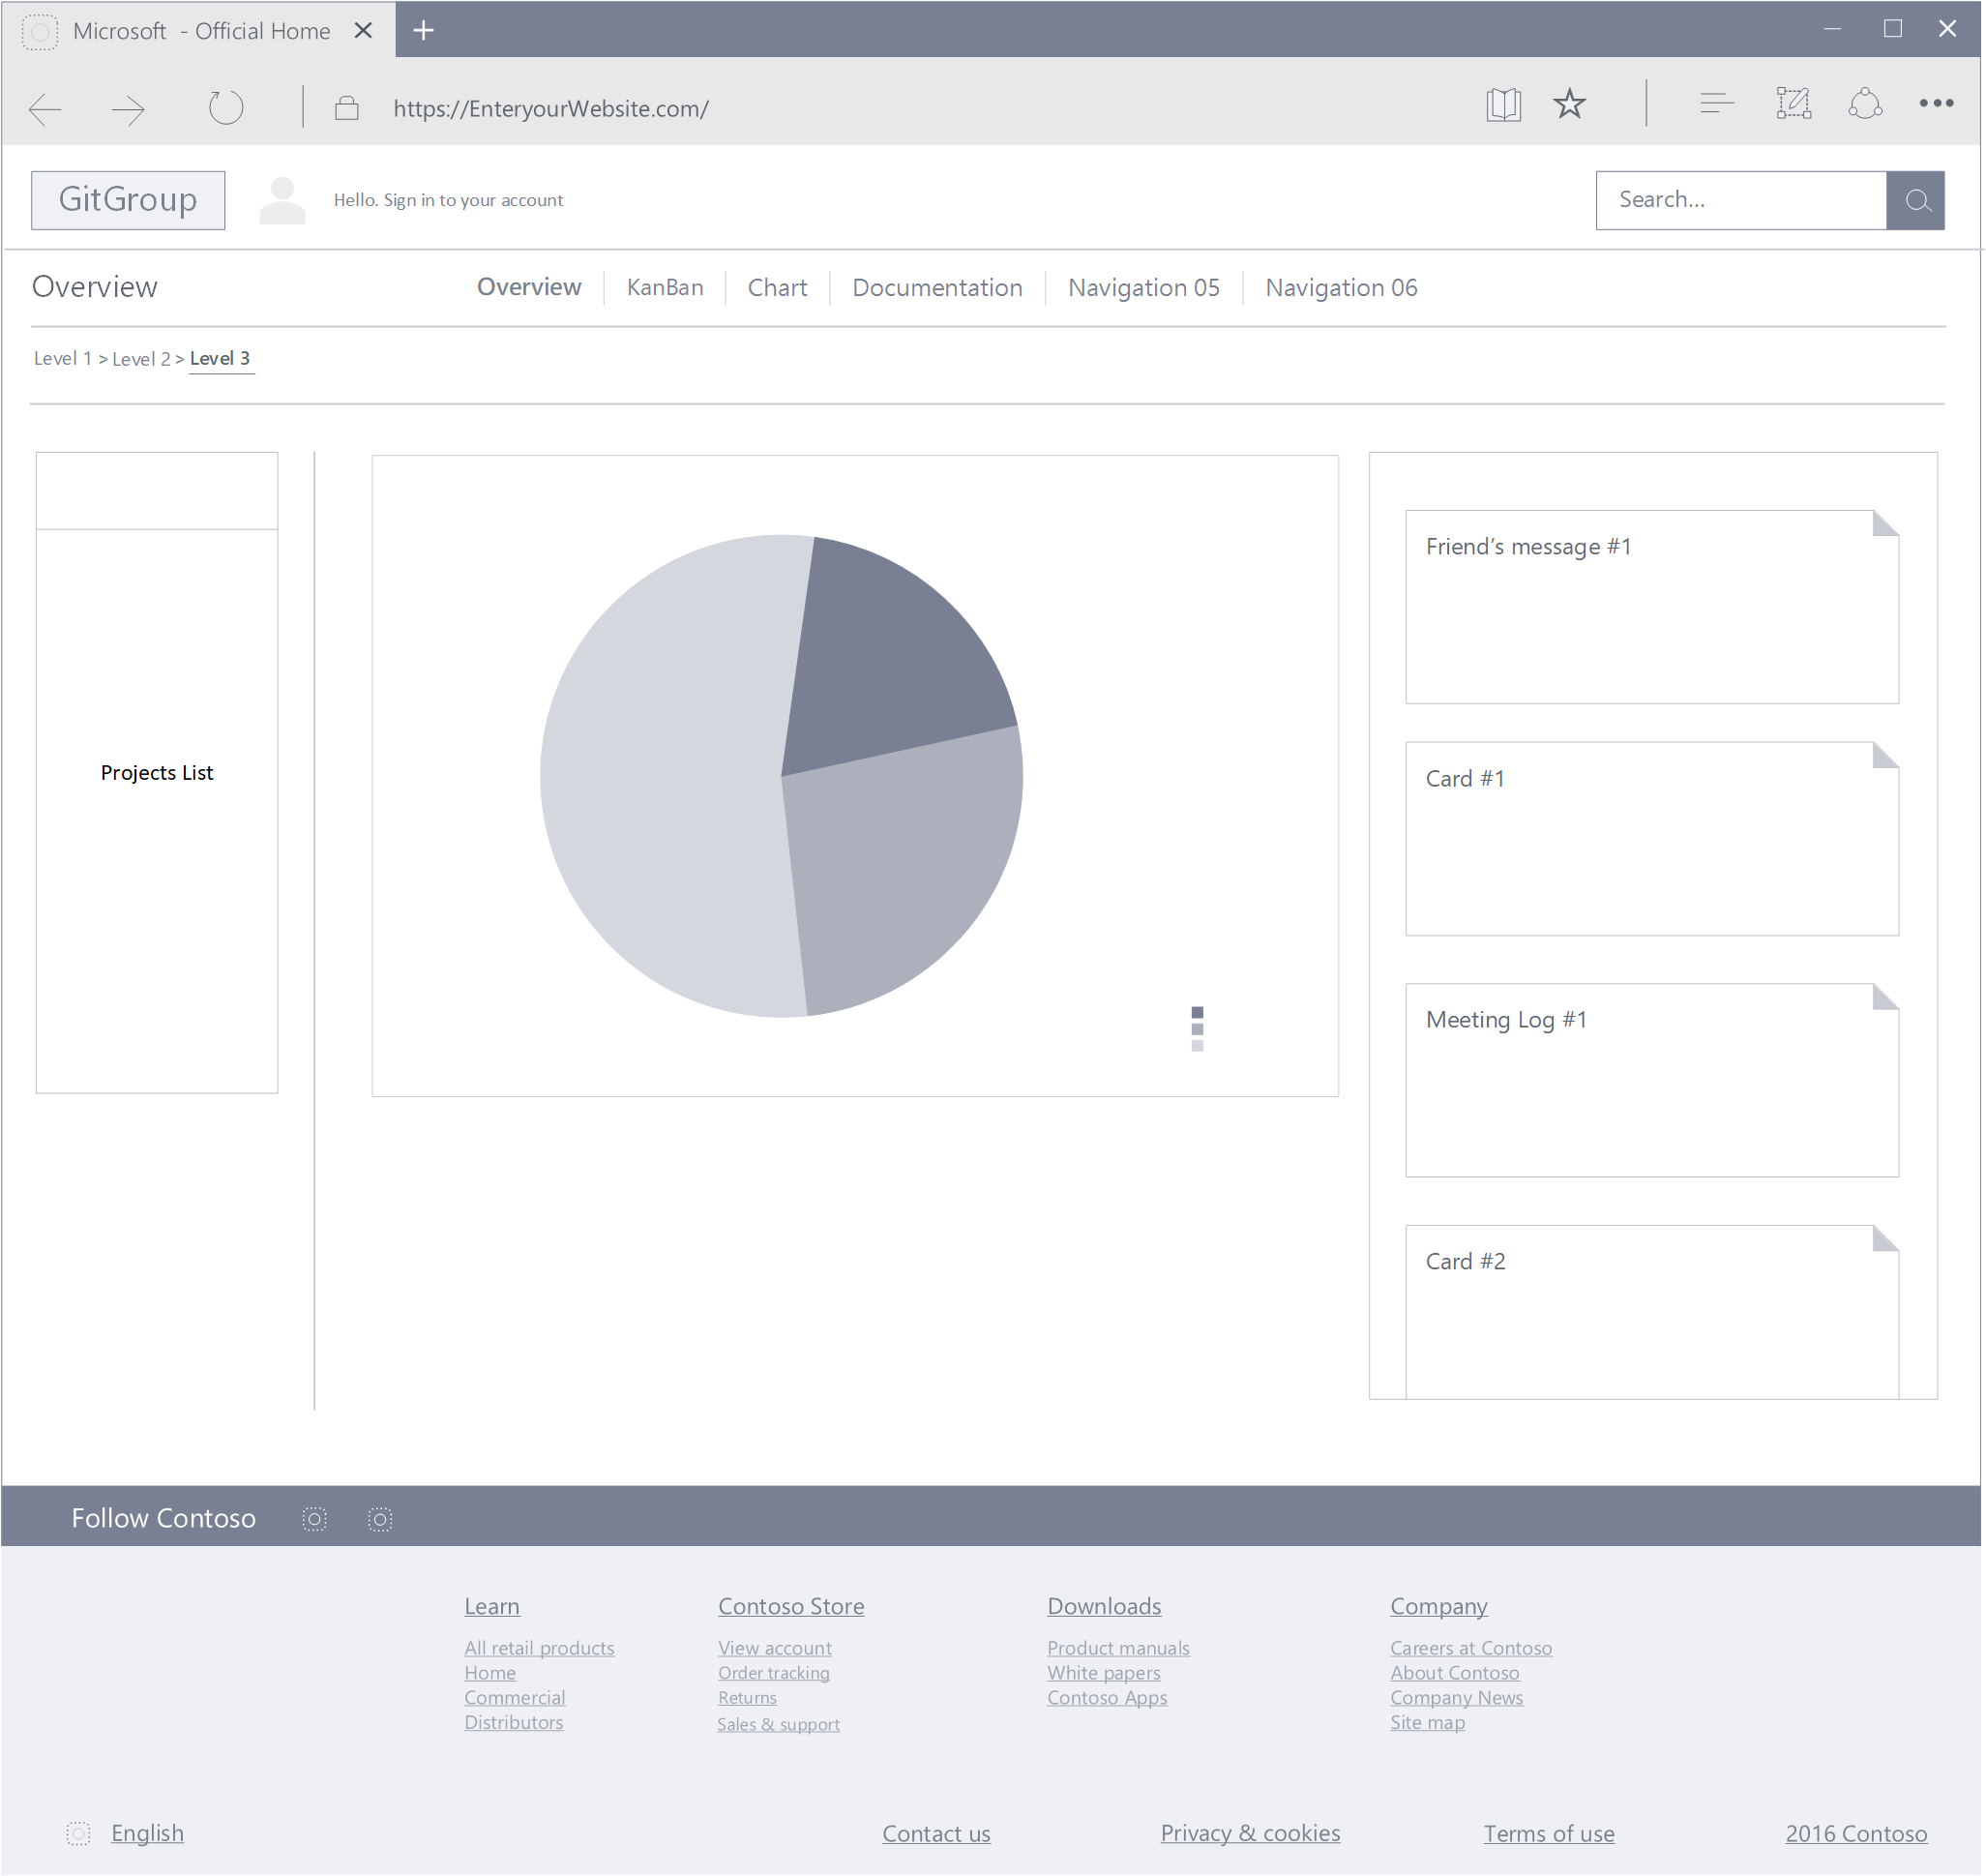
\includegraphics[width=0.6\textwidth]{./pics/OverviewInterface.png}
	\caption{Overview User Interface (Details in Appendix A)}
\end{figure}
The overview is the home page of GitGroup. Because our design aim is ease and simple, all the important information should display on this main page. The main navigation bar shows the personal information. and the second navigation bar is used for navigate among the Overview, Kanban, Chart and Documentation page. The next line is the tool bar, all the tool button should be here. Specially, the left side in this line is the bread crumb which is used to improve the navigation experience. 
The most important part is the workspace which is divided into 3 parts. The left side bar is the Project list where users can search, choose, edit, add and remove project. The combination of the project list and second navigation bar, which is called two-dimension navigation, is stronger, more accurate. \\
The middle part of workspace is user's current status, and it is shown as some diagrams and charts.\\
The right side bar is all the to-do things including cards which are close to deadline, message and meeting log.\\
\begin{figure}[H]
	\centering
	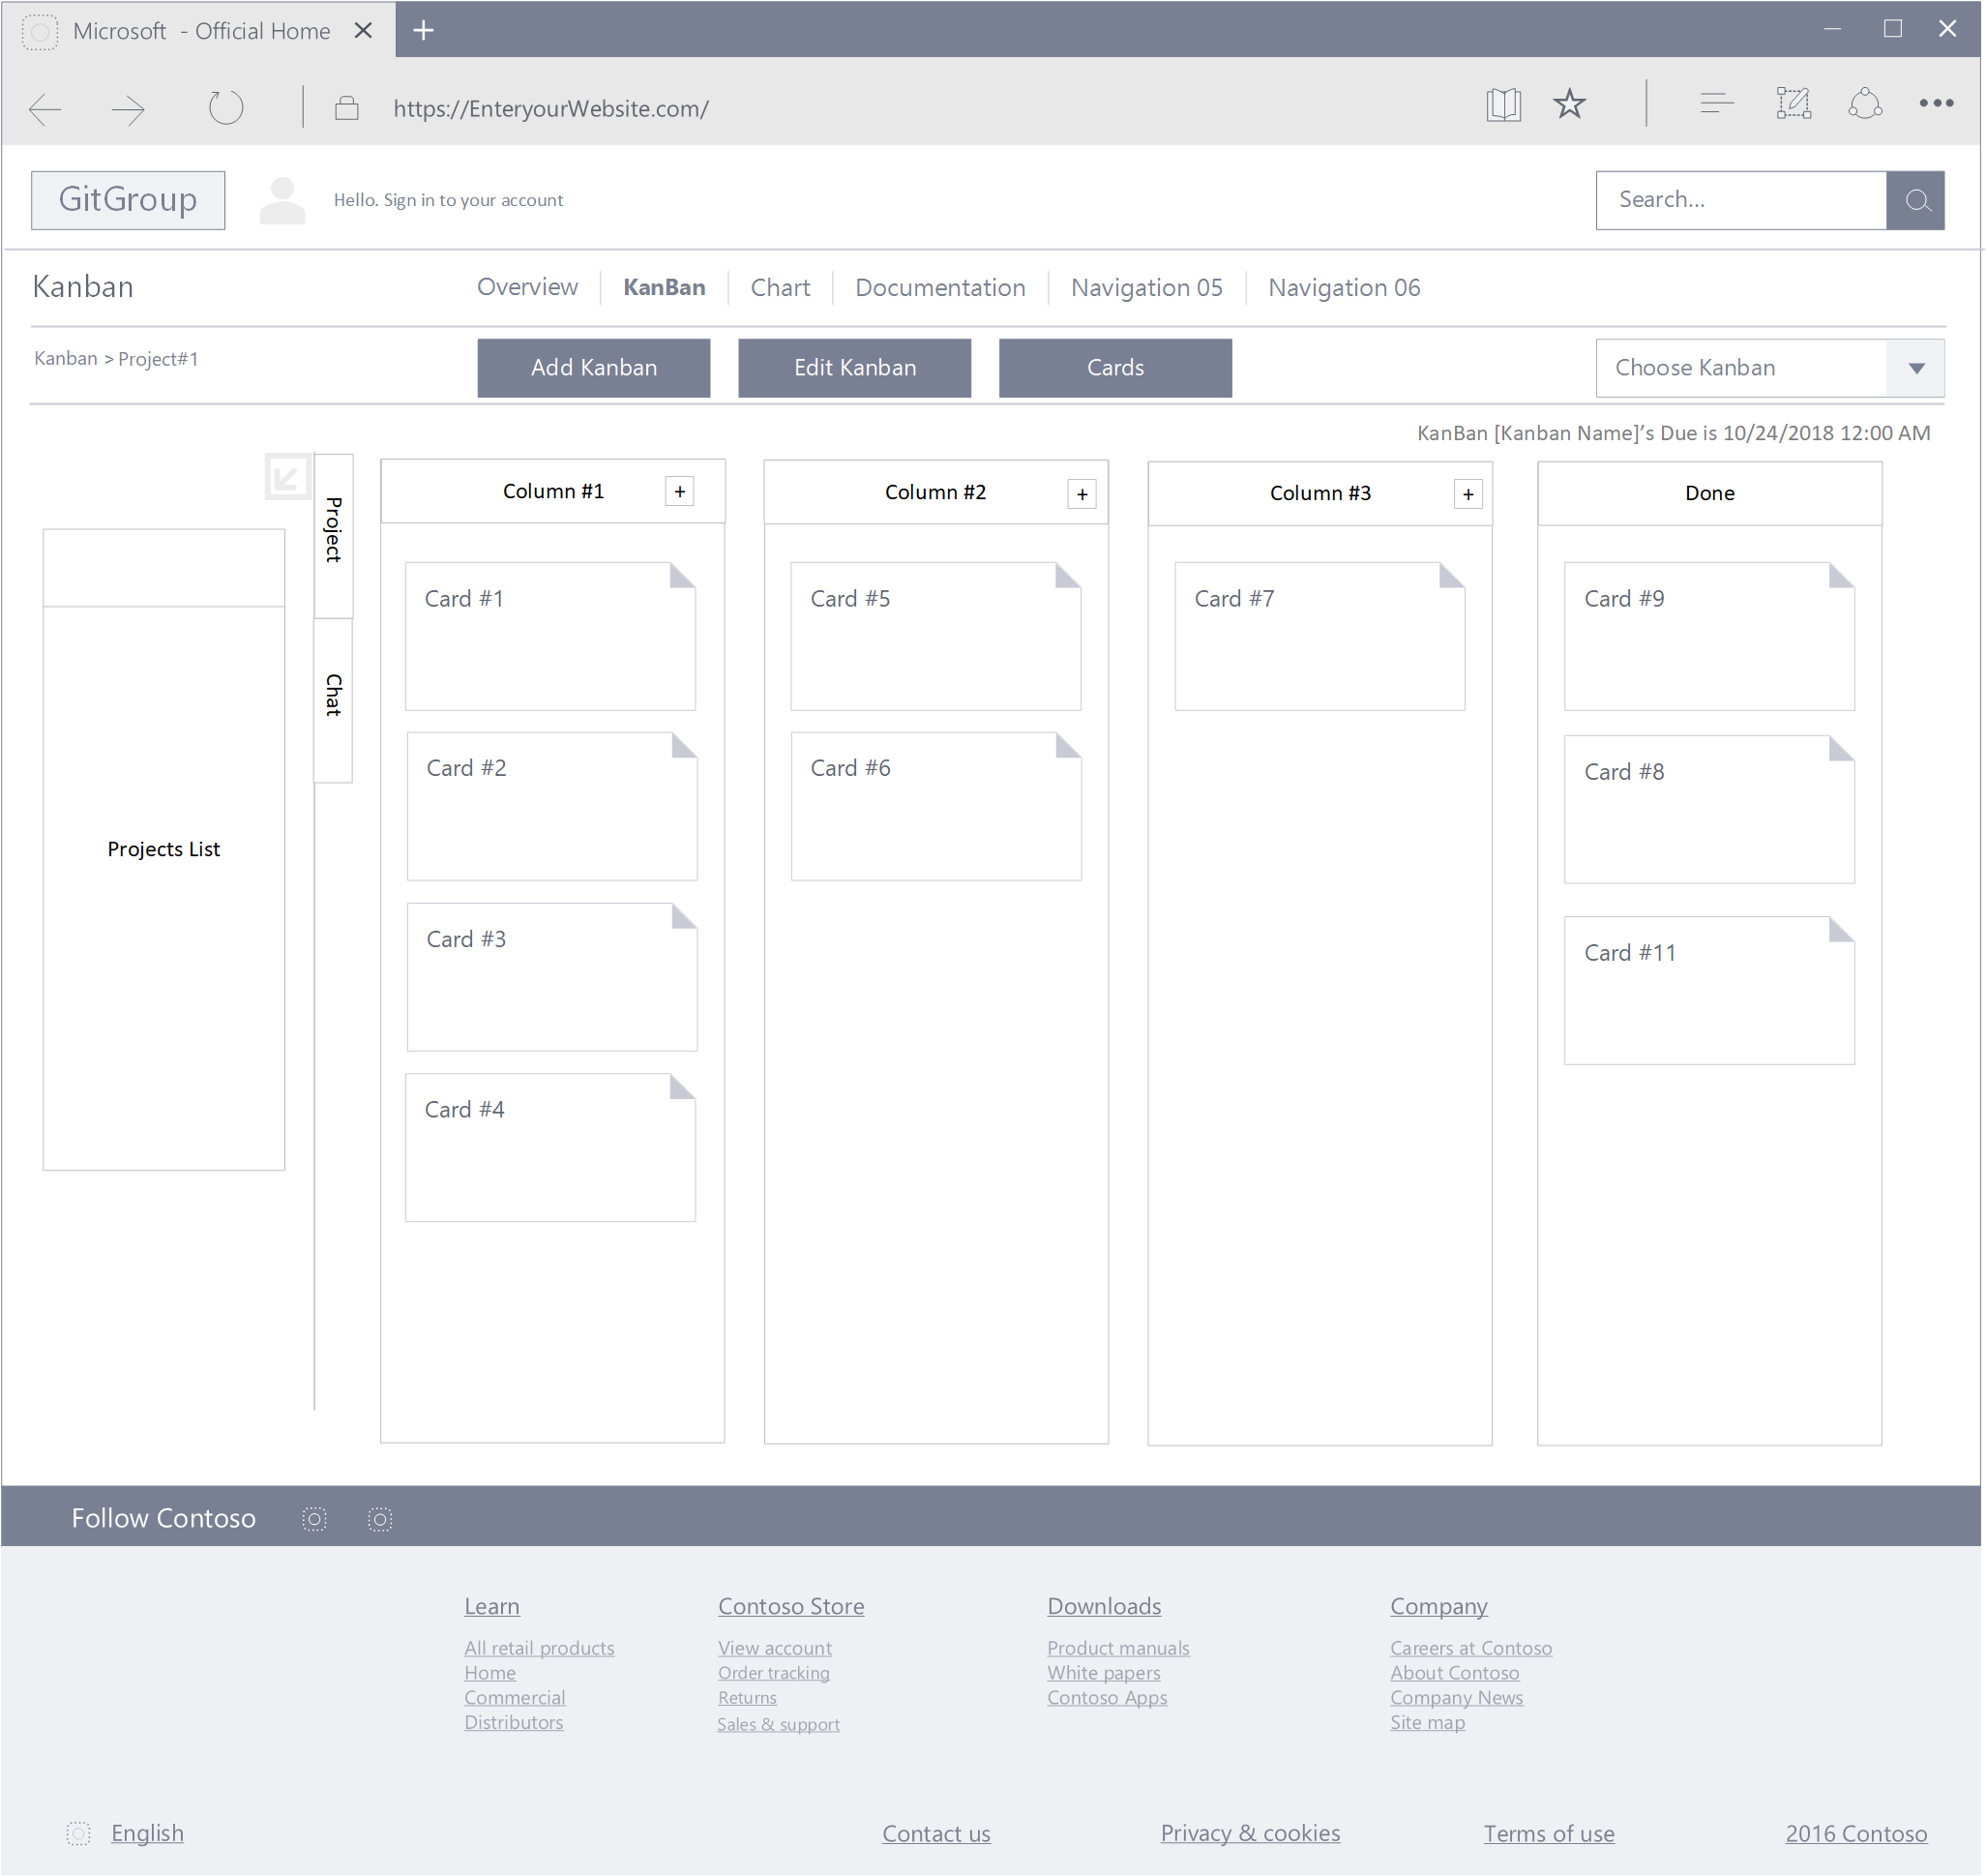
\includegraphics[width=0.6\textwidth]{./pics/KanbanInterface.png}
	\caption{KanBan User Interface (Details in Appendix A)}
\end{figure}
The Kanban board is set of columns that allow you to track the progress of tasks as they move through your workflow. The GitGroup Kanban board default columns are Inbox, Backlog, Ready, In Progress, In Review and Done. Cards that are newly added to the Workspace (such as when an issue is made on GitHub) will go into the Inbox column by default. Cards that are moved into the Done column on GitGroup will be automatically closed and cards closed via GitHub will be automatically moved into the Done column. And the right top of Kanban board shows the due day of this KanBan. 
\begin{figure}[H]
	\centering
	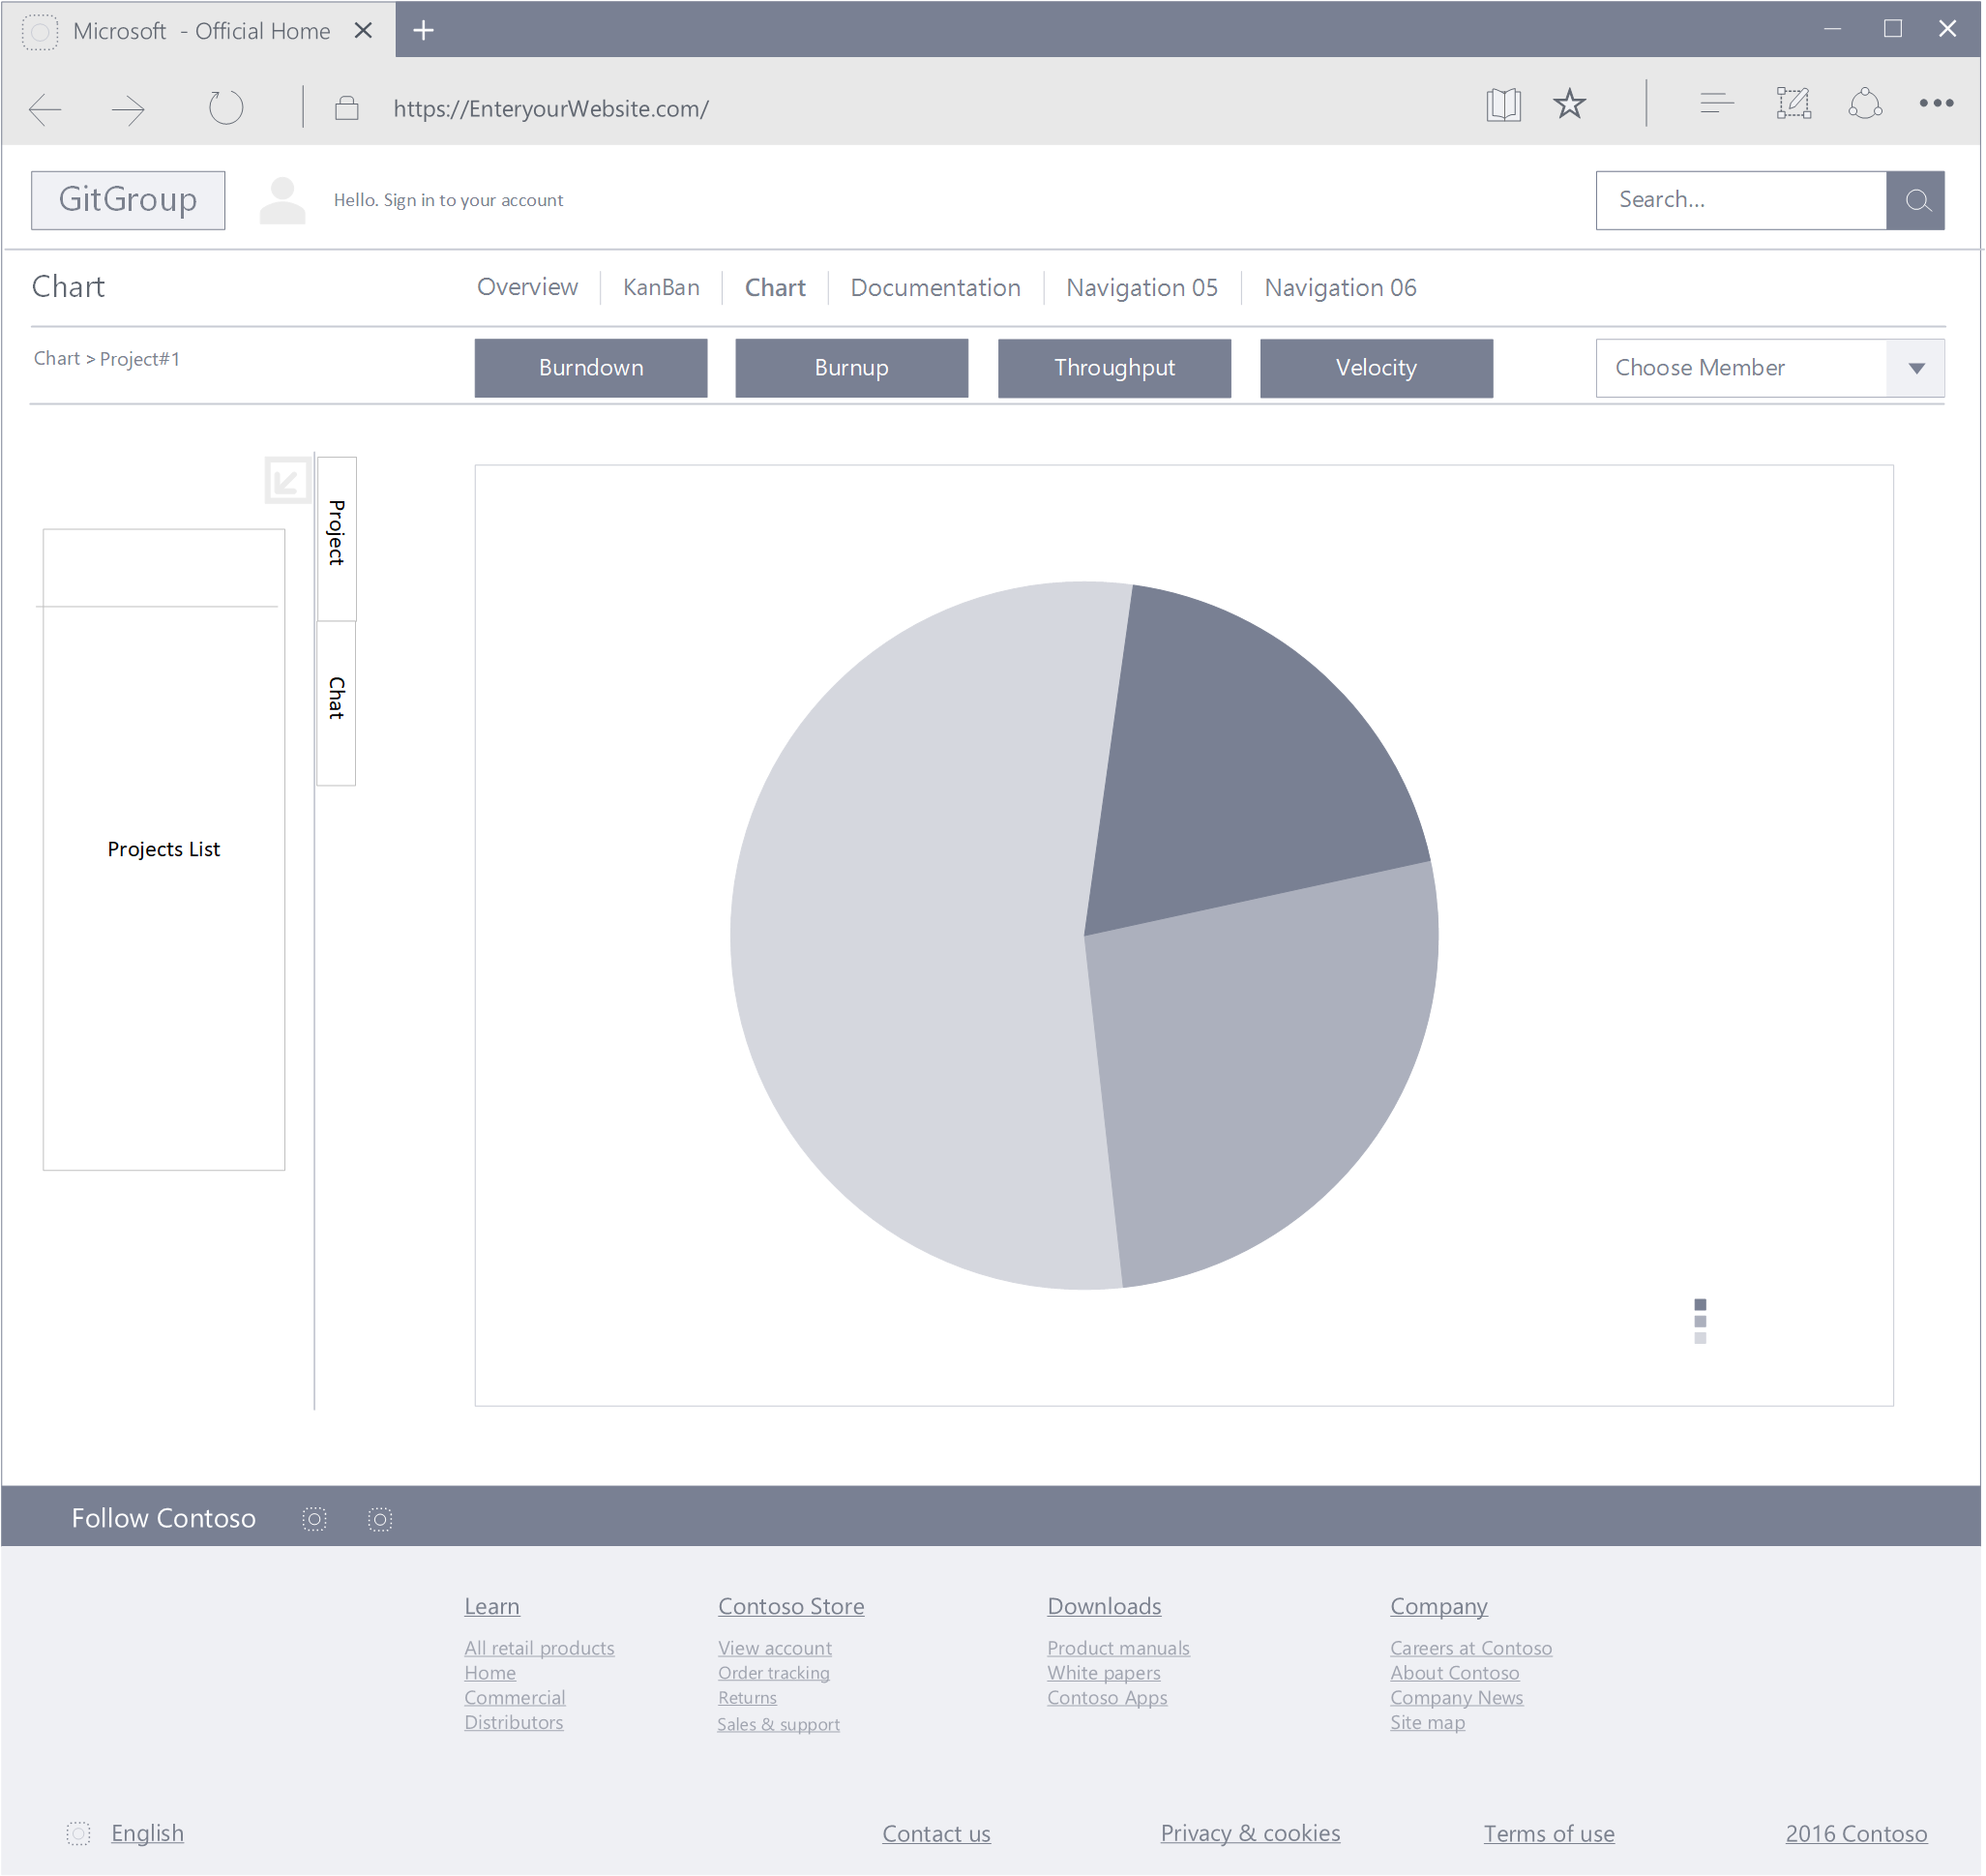
\includegraphics[width=0.6\textwidth]{./pics/ChartInterface.png}
	\caption{Chart User Interface (Details in Appendix A)}
\end{figure}
The Chart UI is easy and understandable. The main part shows different charts and you can change them via buttons on the tool bar.
\section{Hardware Interfaces}
Owing to the responsive nature of the product, it would require nothing more than a simple browser installed on a mobile phone, a tablet or a personal computer. A reasonable amount of RAM on the device would be enough to support the browser and the associated product.
\section{Software Interfaces}
The product will use certain 3rd party libraries or api?s to supplement overall system functionality. The google maps api is used for geocoding street addresses to geographical coordinates that can be used to place markers on the map. These markers provide visual representation for locating parking spaces for drivers. Api?s for financial transactions will be used by the product for booking spots. Communication between the core-application and the api implementation normally happens through SOAP messages.  \\
Software interacts with the database using JSON objects. MongoDB, the primary database vendor stores these objects in binary encoded form called BSON (or Binary JSON). The underlying operating system that runs the application server (web host) will be Linux. 
\section{Communication Interfaces}
The product will make use of a set of communications interface standards. They are summarized below,
\begin{enumerate}
	\renewcommand{\labelenumi}{{\textbf{\arabic{enumi}.}}}
	\item Emails are sent to drivers when a booking has been made. Similarly, owners receive booking information through email when drivers reserve parking spots. These features depend on application layer protocols like SMTP and IMAP for their implementation.
	\item Client-Server communication needs to be encrypted in order to ensure secure data transfer. Thus, we require a HTTPS/SSL (or TLS) connections between the client and server always.
	\item Electronic payments for booking and confirmation must be implemented using secure, encrypted VPN tunnels. This responsibility will be relegated to the payment gateway service provider.  
\end{enumerate}


% -----------------------------------------------------
% Chapter 4 Requirements
% -----------------------------------------------------
\chapter{Requirements}
\section{User Requirements}
	\subsection{Functional User Requirement}
		\begin{enumerate}
			\renewcommand{\labelenumi}{{\textbf{\arabic{enumi}.}}}
			\item User shall be able to create a new project and new team in GitGroup.
			\item User shall be able to manage GitHub repositories and team members like add or remove repositories and members.
			\item User shall be able to use Kanban board to organize issues by dragging issue cards among several columns representing different stage of the development processes.
			\item User shall be able to analysis the development duration, quality and the team work situation of the project by using a variety of agile charts and analytics.
			also manage tasks like suggesting a new idea or tracking a bug. 
			\item User shall be able to organize an online meeting group chat, schedule and record the conference within the team or the global scope.
		\end{enumerate}
	\subsection{Non-Functional User Requirement}
		\begin{enumerate}
			\renewcommand{\labelenumi}{{\textbf{\arabic{enumi}.}}}
			\item The application shall be able to make GitHub easy to use, especially friendly for the person who has little development experience such as product manager.
			\item The application shall be quickly restored to operational status after a failure occurs.
			\item The app shall be reliable to uses with no downtime.
			\item The application shall be able to provide maximum security against malicious attack.
		\end{enumerate}
\section{System Requirements}
	\subsection{Functional System Requirement}
		\begin{enumerate}
			\item[\textbf{1.1}] Developers can create a new project and make a team with other developers.
			\item[\textbf{1.2}] Developers can remove a project and collaborators of the project after checking if the project is empty.
			\item[\textbf{2.1}] Developers can manage their team by inviting to or removing collaborators from their projects.
			\item[\textbf{2.2}] Developers can manage their repositories by adding or removing repositories of their projects.
			\item[\textbf{3.1}] Developers can classify issues by different stages of development process via putting them in different columns of Kanban board. 
			\item[\textbf{3.2}] Developers can add or remove a Kanban from their Kanban board.
			\item[\textbf{3.3}] Developers can customize their own stage by editing column name except Done column.
			\item[\textbf{3.4}]	Developers can close issues by dragging it to the Done column, which will automatically close issues in the GitHub. 
			\item[\textbf{4.1}] Project manager can track and communicate the progress of their projects by burn down and burn up charts.
			\item[\textbf{4.2}] Project manager can measure how much work a team can used in eXtreme Programming and Scrum from throughput chart.
			\item[\textbf{4.3}] Project manager can analysis the velocity of project going from velocity chart.
			\item[\textbf{5.1}] Team leader can organize an online meeting group chat within their team.
			\item[\textbf{5.2}] Developers can organize an online meeting group chat within the global.
			\item[\textbf{5.3}] Developers can receive a meeting notification from team leader.
			\item[\textbf{5.4}] Developers can set an alarm for notifying the coming events on a conference schedule form.
			\item[\textbf{5.5}] Developers shall be able to record content of meeting on a meeting notebook.
		\end{enumerate}
	\subsection{Non-Functional System Requirement}
		\begin{enumerate}
			\item[\textbf{1.1}] The user shall be able to use all the app functions without any kind of training. The average number of questions call about how to use app shall not exceed 10 per day.
			\item[\textbf{1.2}] The app shall be available for any kind of mobile device and PC.
			\item[\textbf{2.1}]
			\item[\textbf{3.1}] The app shall be available to all users during whole day (Mon-Sun, 00:00~00:00)
			\item[\textbf{4.1}] The app shall not expose contact information to other users. 
			\item[\textbf{4.2}] The app should minimize the amount of personally identifying information (PII) that it collects.
		\end{enumerate}
	
% ------------------------------------------------------
% Chapter 5 System Models
% ------------------------------------------------------
\chapter{System Models}
\section{Use Case Diagram}
A use case diagram at its simplest is a representation of a user's interaction with the system that shows the relationship between the user and the different use cases in which the user is involved. A use case diagram can identify the different types of users of a system. There are two type user in GitGroup that are owner and collaborator. Both of them can use KanBan, view charts, and do chat. But the owner have higher privilege, they have the permission to invite or remove collaborator, delete the project or create and remove KanBan etc.
\begin{figure}[H]
	\centering
	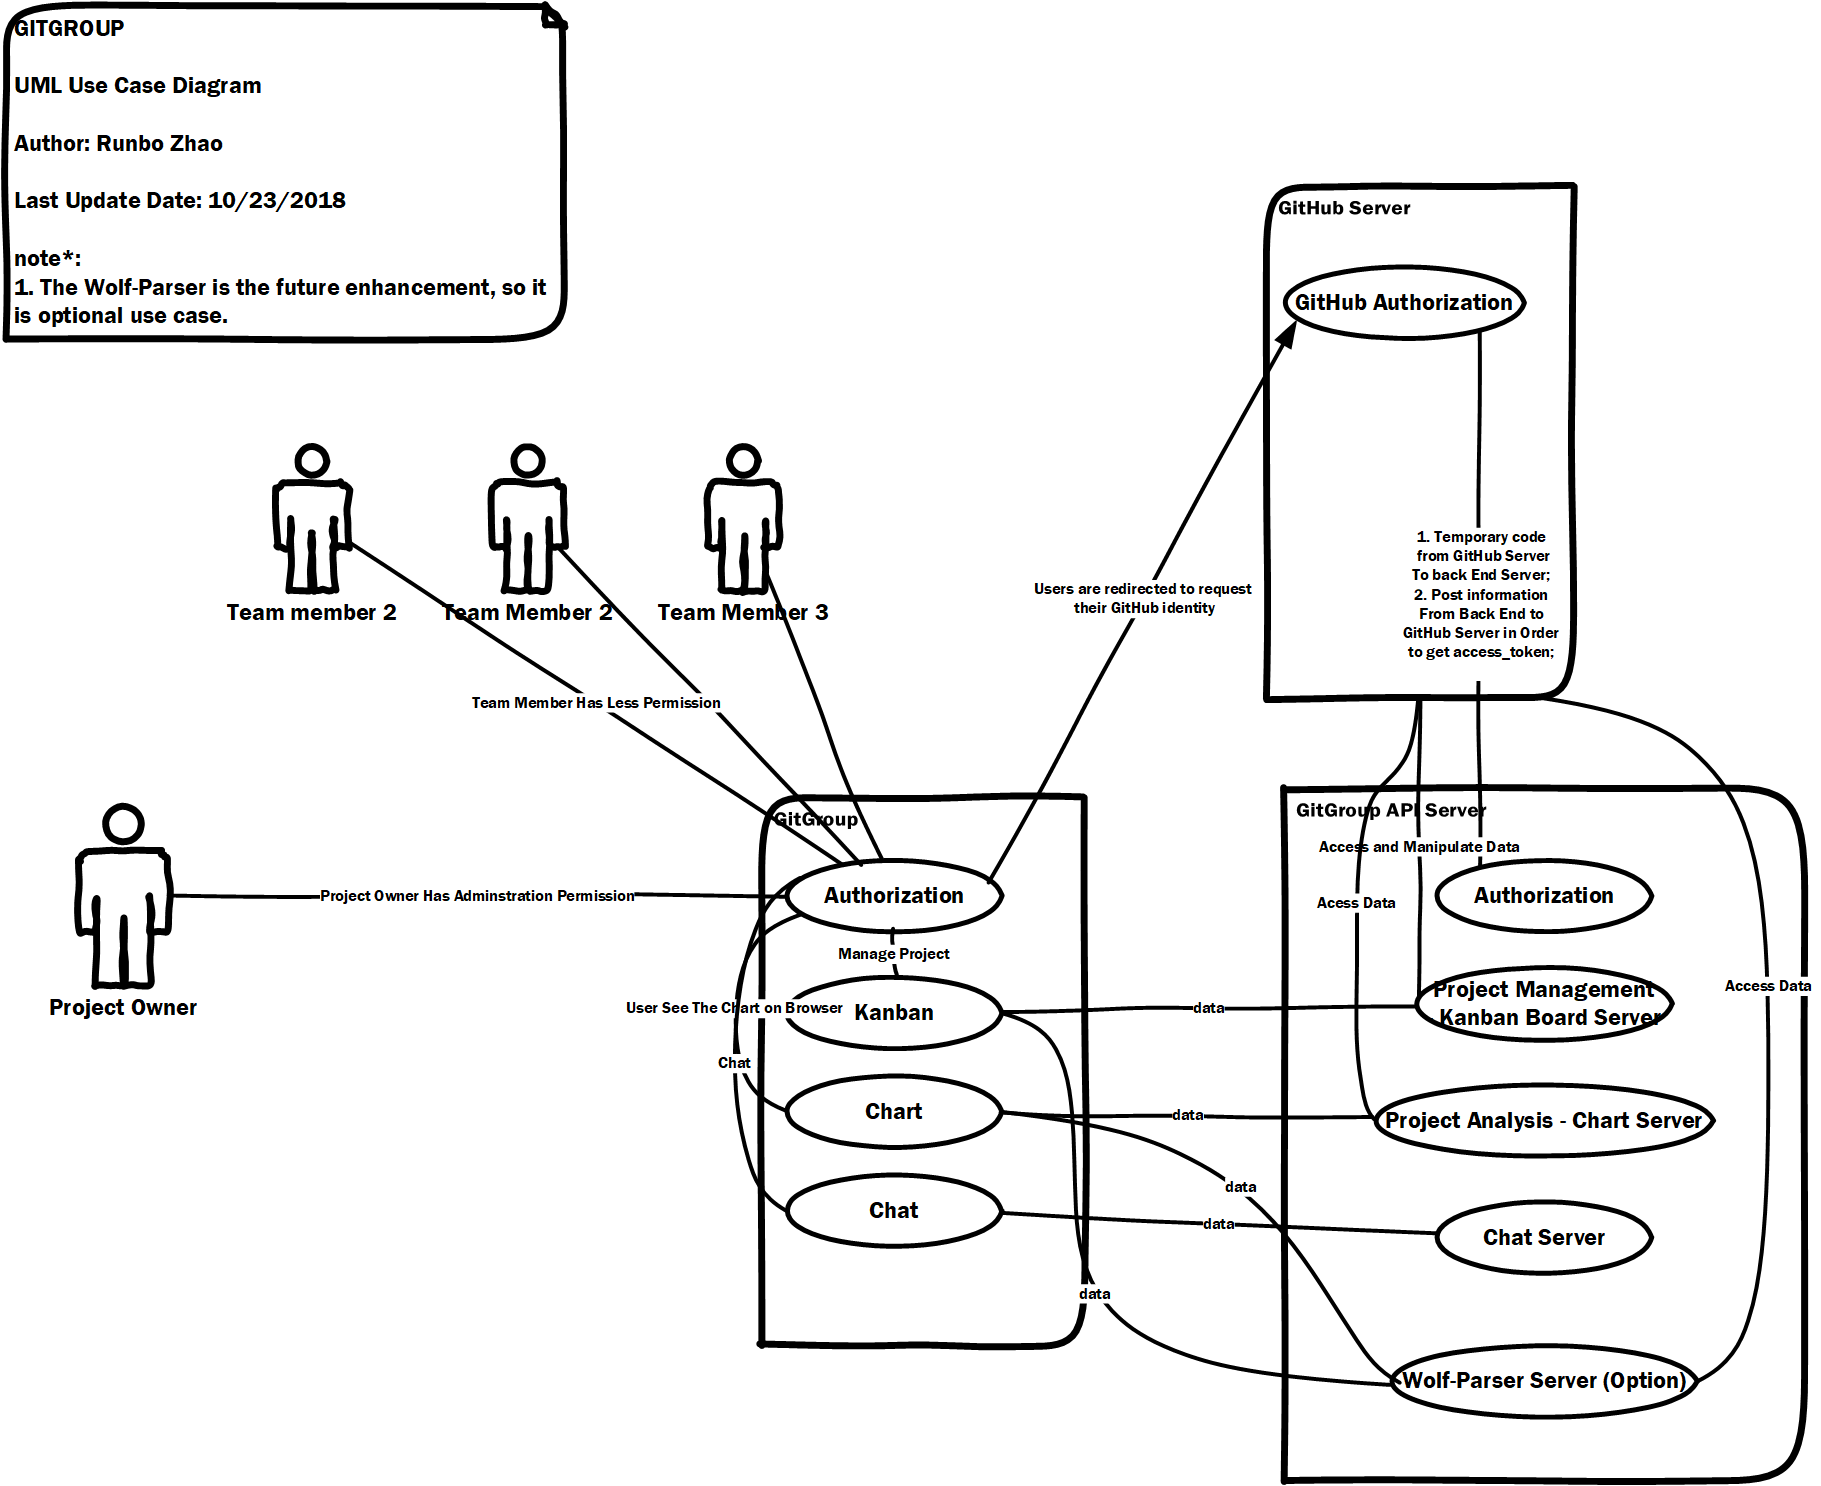
\includegraphics[width=0.7\textwidth]{./pics/UseCaseDiagram.png}
	\caption{Use Case Diagram}
\end{figure}
\subsection{KanBan}
The Kanban board which is similar to projects board in the Gitub. In the Kanban board, there are several columns represent different stage of the developement process, such as TODO, Ready, In Progress, Done... You can customize your own stage. Both owner and collaborators can access KanBan, However the owner has higher privilege.\\
Every column contains issue card imported from the Github, and you can easily drug them among the columns. If you drug it to the Done column. The issue in the Github will be automatically closed.
\subsection{Chart}
GitGroup offers a variety of Agile charts and analytics to help you keep track of how your team is doing. Both owner and collaborators can view these charts.
\begin{enumerate}
	\renewcommand{\labelenumi}{{\textbf{\arabic{enumi}.}}}
	\item Burndown and Burnup Charts\\
	A Burnup chart tracks how much work has been completed during the Sprint. Burnup charts have three lines, Goal, Closed Points/Cards, and Ideal Closed Points/Cards. The Goal line allows you to easily see when new work is added to a sprint. Similar to the Burndown Ideal line, the Burnup ideal line marks how much work should have been closed in order to ensure all of the work in your Sprint is completed on time. The Closed line shows the total number of points or cards closed that have been closed. \\
	Both Burndown and Burnup charts can be filtered by source and can be set to exclude weekends in the Ideal line calculation. They can also display data using point totals or card totals. 
	\item Throughput Chart\\
	The Throughput chart shows you how much work your team is completing everyday. The chart is a stacked bar chart with each segment representing the work done on each of your sources. Throughput charts can help you spot changes in your team's productivity or workflow. Zube's Throughput chart has many filters that allow you dig into the details of what work is being completed everyday.\\ 
	The Throughput chart can be filtered by card type, source, assignee, epic, label, milestone and sprint. You can also adjust the date range displayed. Data can be presented as point totals or card totals. 
	\item Users Throughput Chart\\
	The Users Throughput chart tracks how much is being done by each team member weekly. Like the Throughput chart, the Users throughput chart allows you to track how efficiently your team is working and spot potential problems in your team members' workflows. The Users Throughput chart also offers a rich set of filters. The chart can be displayed as a stacked area chart or stacked bar chart. \\
	The Users Throughput chart can be filtered by source, assignee, label, milestone and sprint. You can also adjust the date range displayed. Data can be presented as point totals or card totals. 
	\item Velocity Chart\\
	If you are using Sprints, you can track how much work your team is getting done per sprint with the Velocity chart. The Velocity chart is a stacked bar chart showing how many cards or points were closed during each sprint in the selected date range. Each section of the bars represents one of your sources. The Velocity chart allows you to see potential problems in your team's efficiency as well as providing a way to predict how much work your team will be able to accomplish in future sprints. \\
	The Velocity chart can be filtered by source and label. You can also adjust the date range displayed. Data can be presented as point totals or card totals. 
\end{enumerate}
\subsection{Chat}
GitGroup offers chat room for users to communication. There are two types of chat. One is global chat which is used to communicate friends directly. Another is in-team chat which is used to communicate among the team members.
\section{State Diagram}
A state diagram, sometimes known as a state machine diagram, is a type of behavioral diagram in the Unified Modeling Language (UML) that shows transitions between various objects. \\ 
The following state diagram shows the transition of the user type. Every use can create their own projects. If they are in their own projects, they are owners, verse and vice, they are collaborator. Therefore, one user can be both owner and collaborator according the project they are managing.\\
\begin{figure}[H]
	\centering
	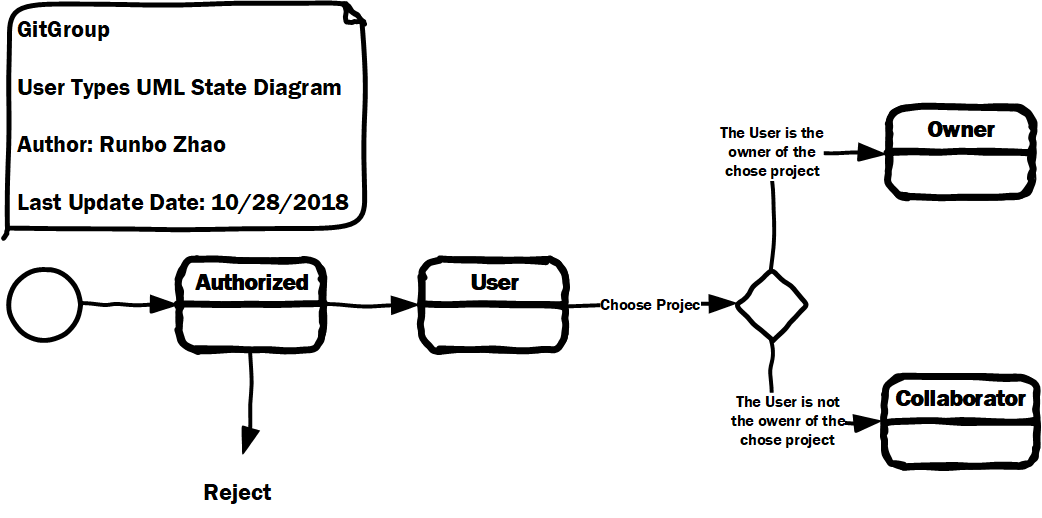
\includegraphics[width=0.7\textwidth]{./pics/UserTypeStateDiagram.png}
	\caption{User Type State Diagram }
\end{figure}
GitGroup offers every project a KanBan board. You can create multiple KanBans for the project and every KanBan has its own due day, after the due day the KanBan will finished no matter how many cards are not finished. These unfinished cards' information is used to analyzed the project development status.\\
In one KanBan, some cards which represent some task flow through a set of step, such as developing, testing, done... . Each moving of a card will change its state in the KanBan.
\begin{figure}[H]
	\centering
	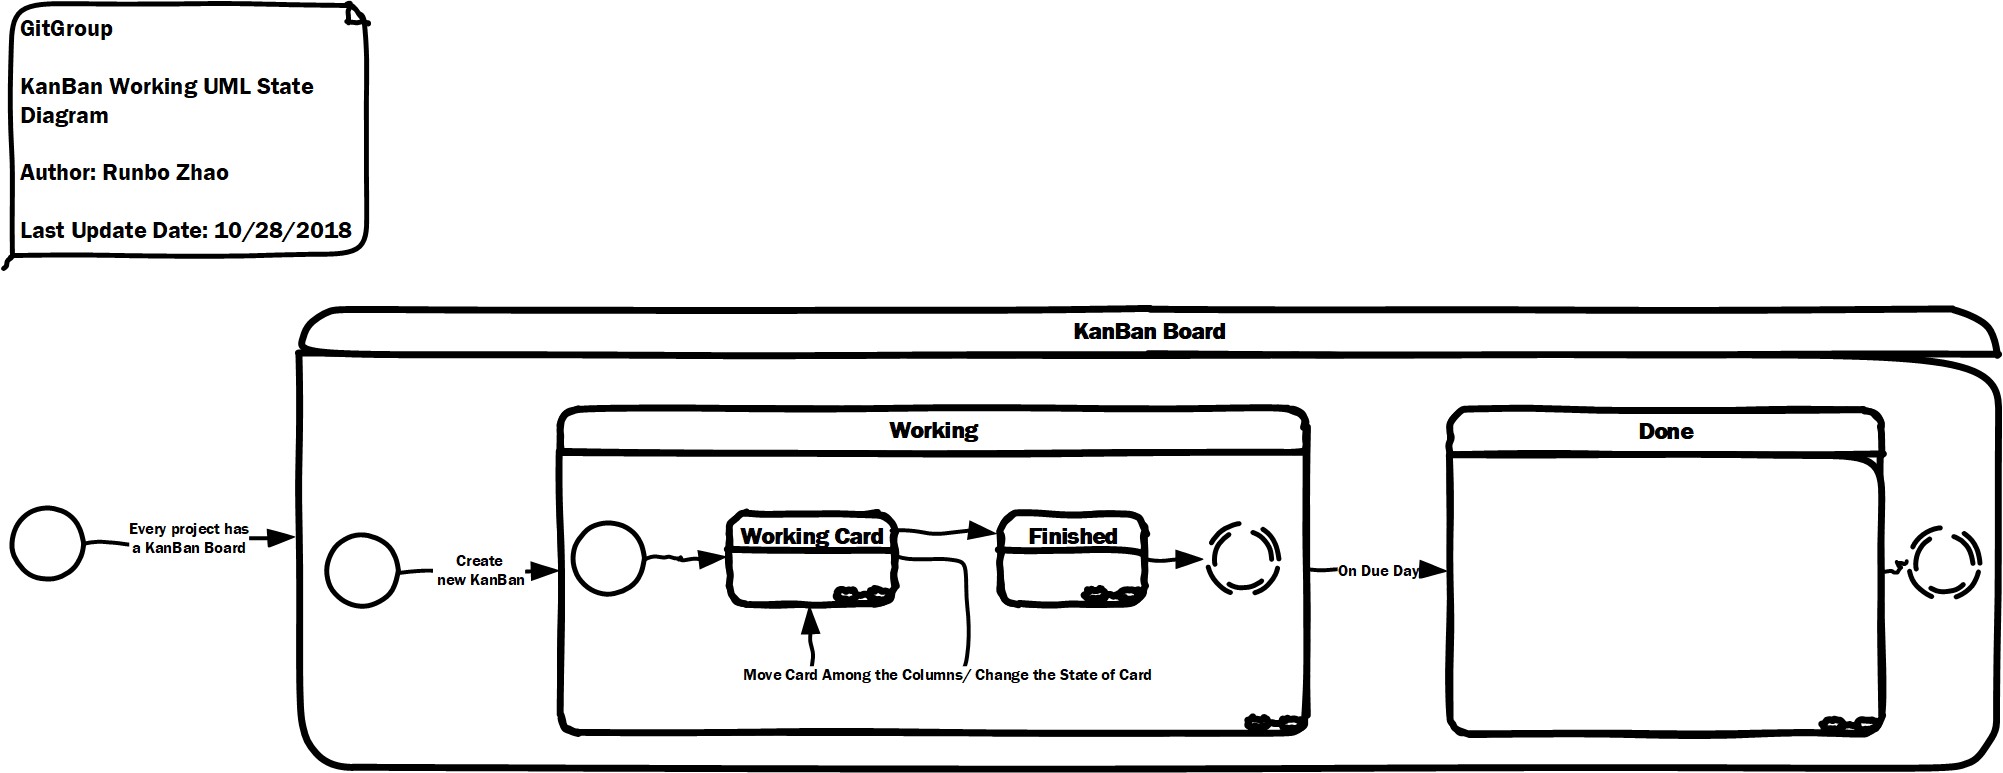
\includegraphics[width=0.8\textwidth]{./pics/KanBanStateDiagram.png}
	\caption{KanBan State Diagram }
\end{figure}
\section{Activity Diagram}
Activity diagram is used to describe the dynamic aspects of the system. Activity diagram is basically a flowchart to represent the flow from one activity to another activity. The activity can be described as an operation of the system.
\begin{figure}[H]
	\centering
	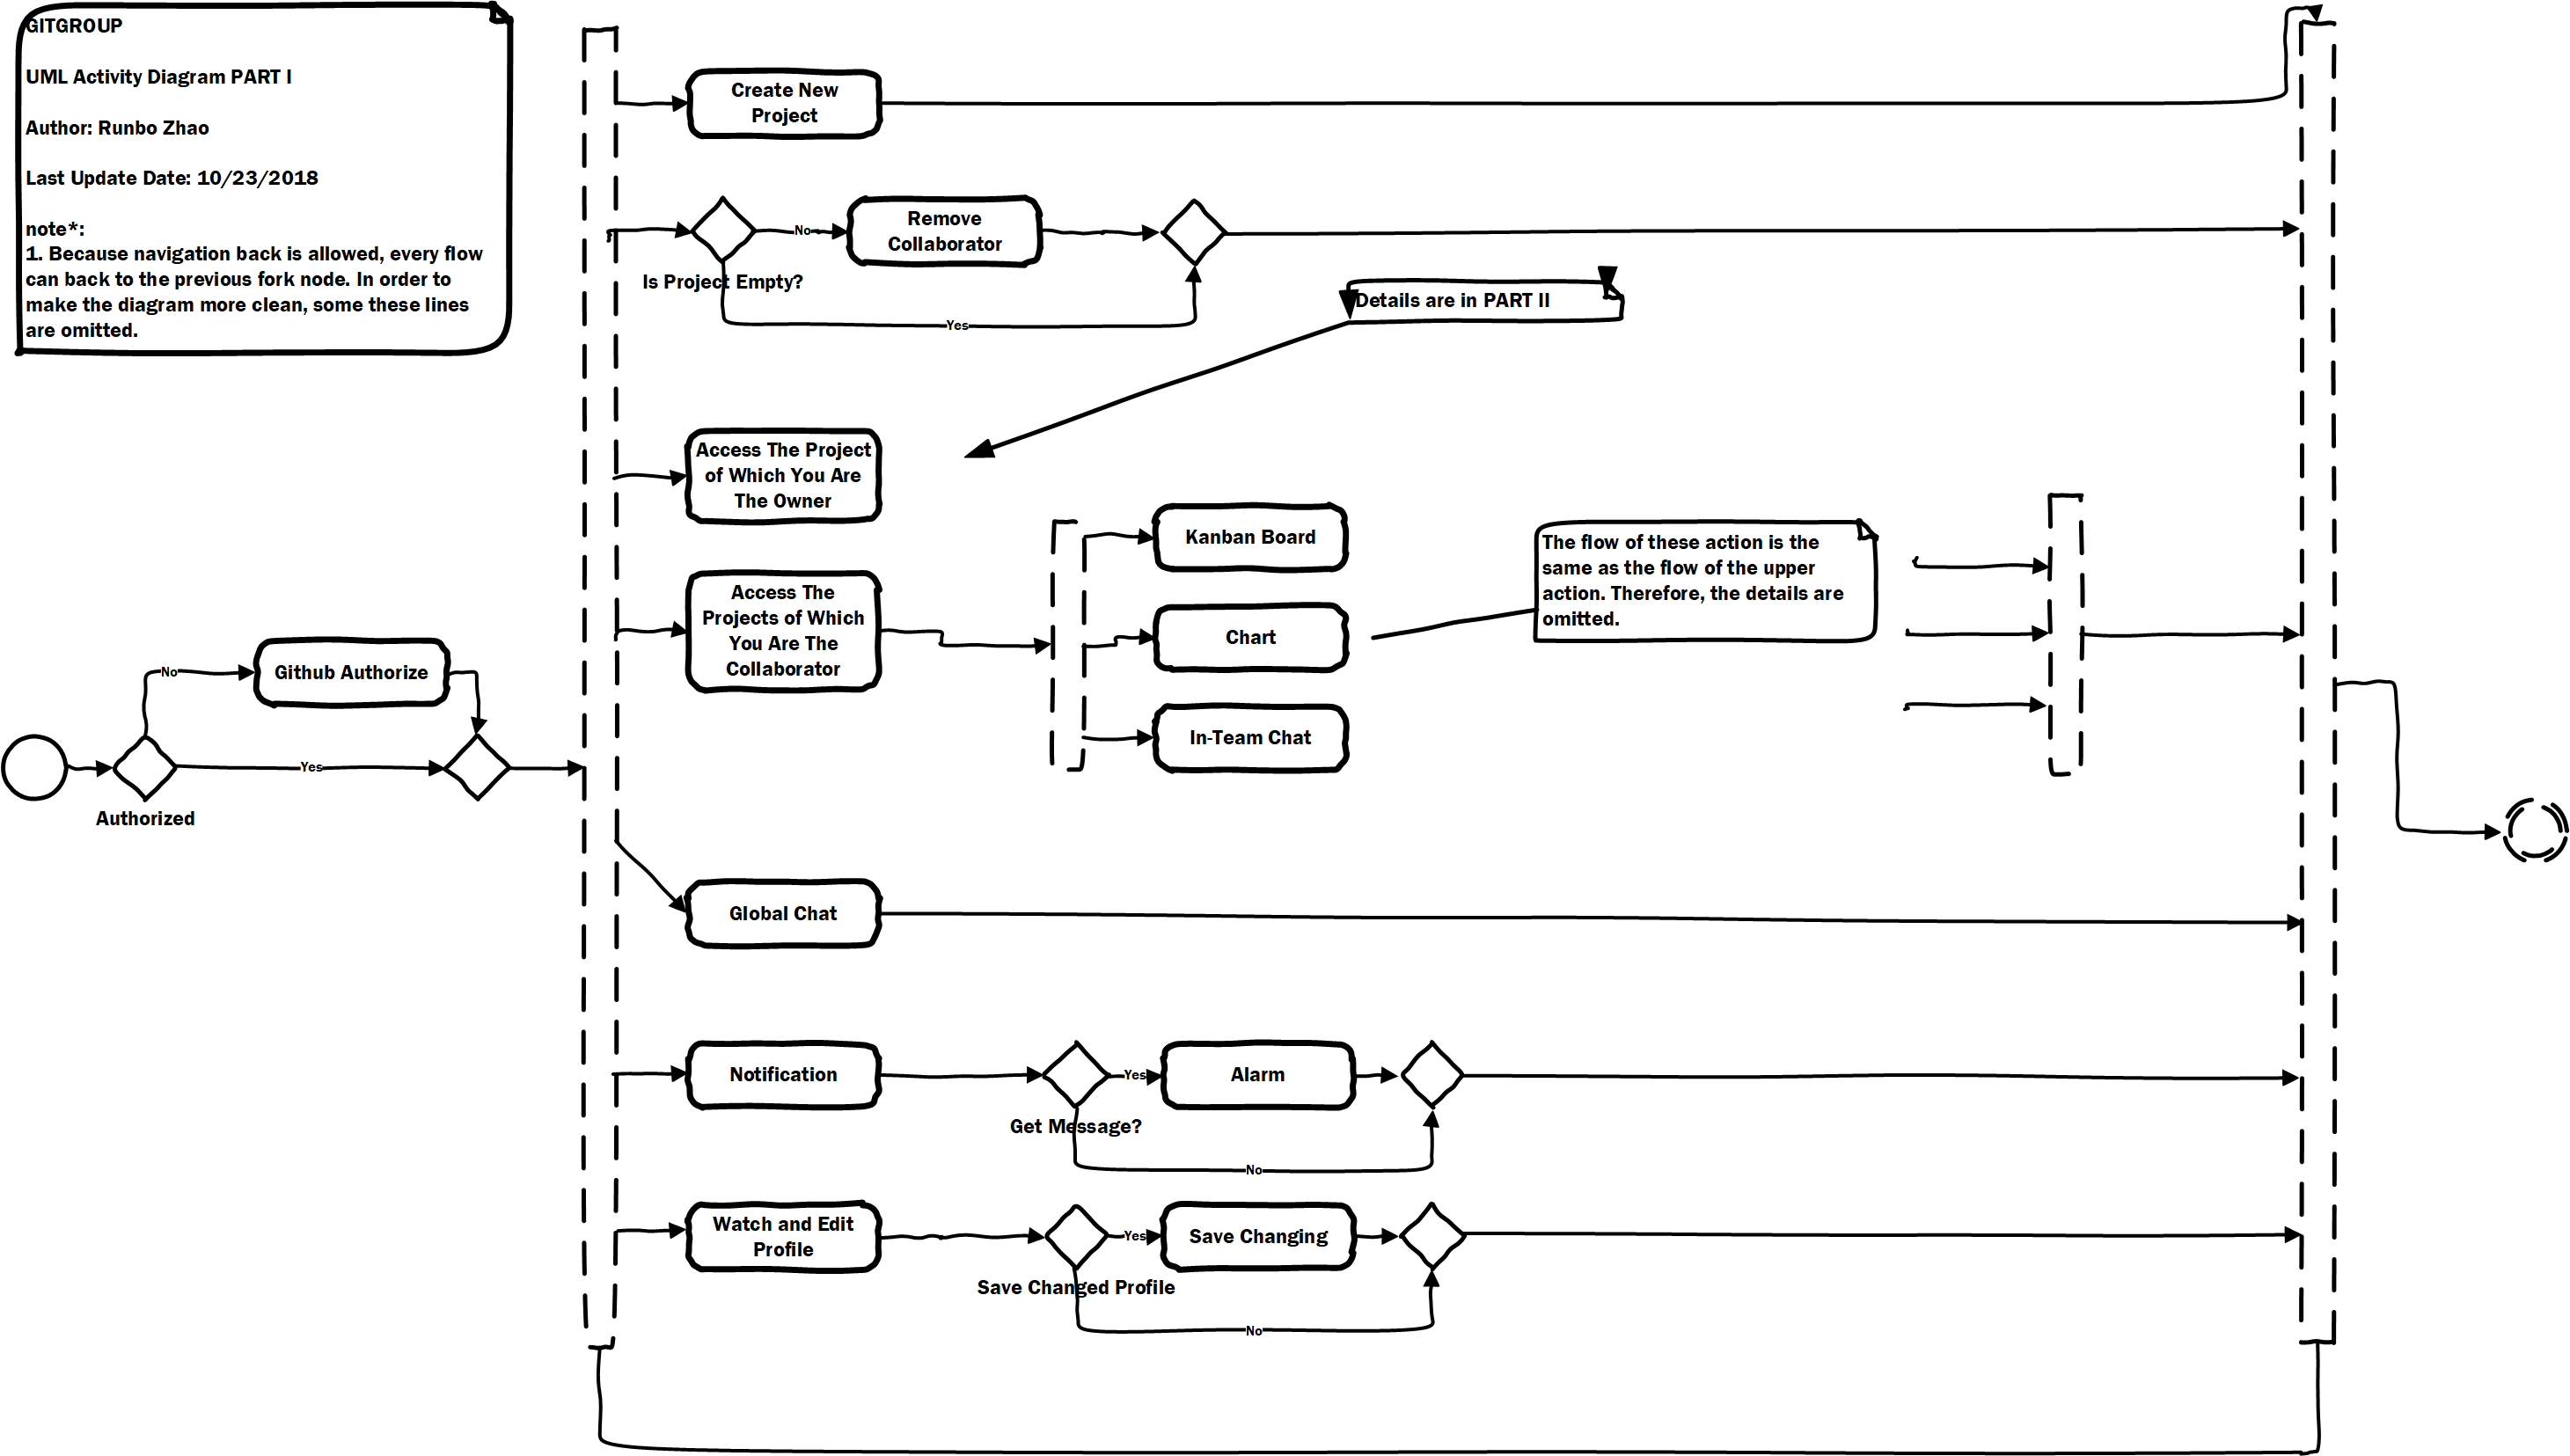
\includegraphics[width=0.7\textwidth]{./pics/ActivatyDiagramPARTI.png}
	\caption{Activity Diagram PART I (Details in Appendix A)}
\end{figure}

\begin{figure}[H]
	\centering
	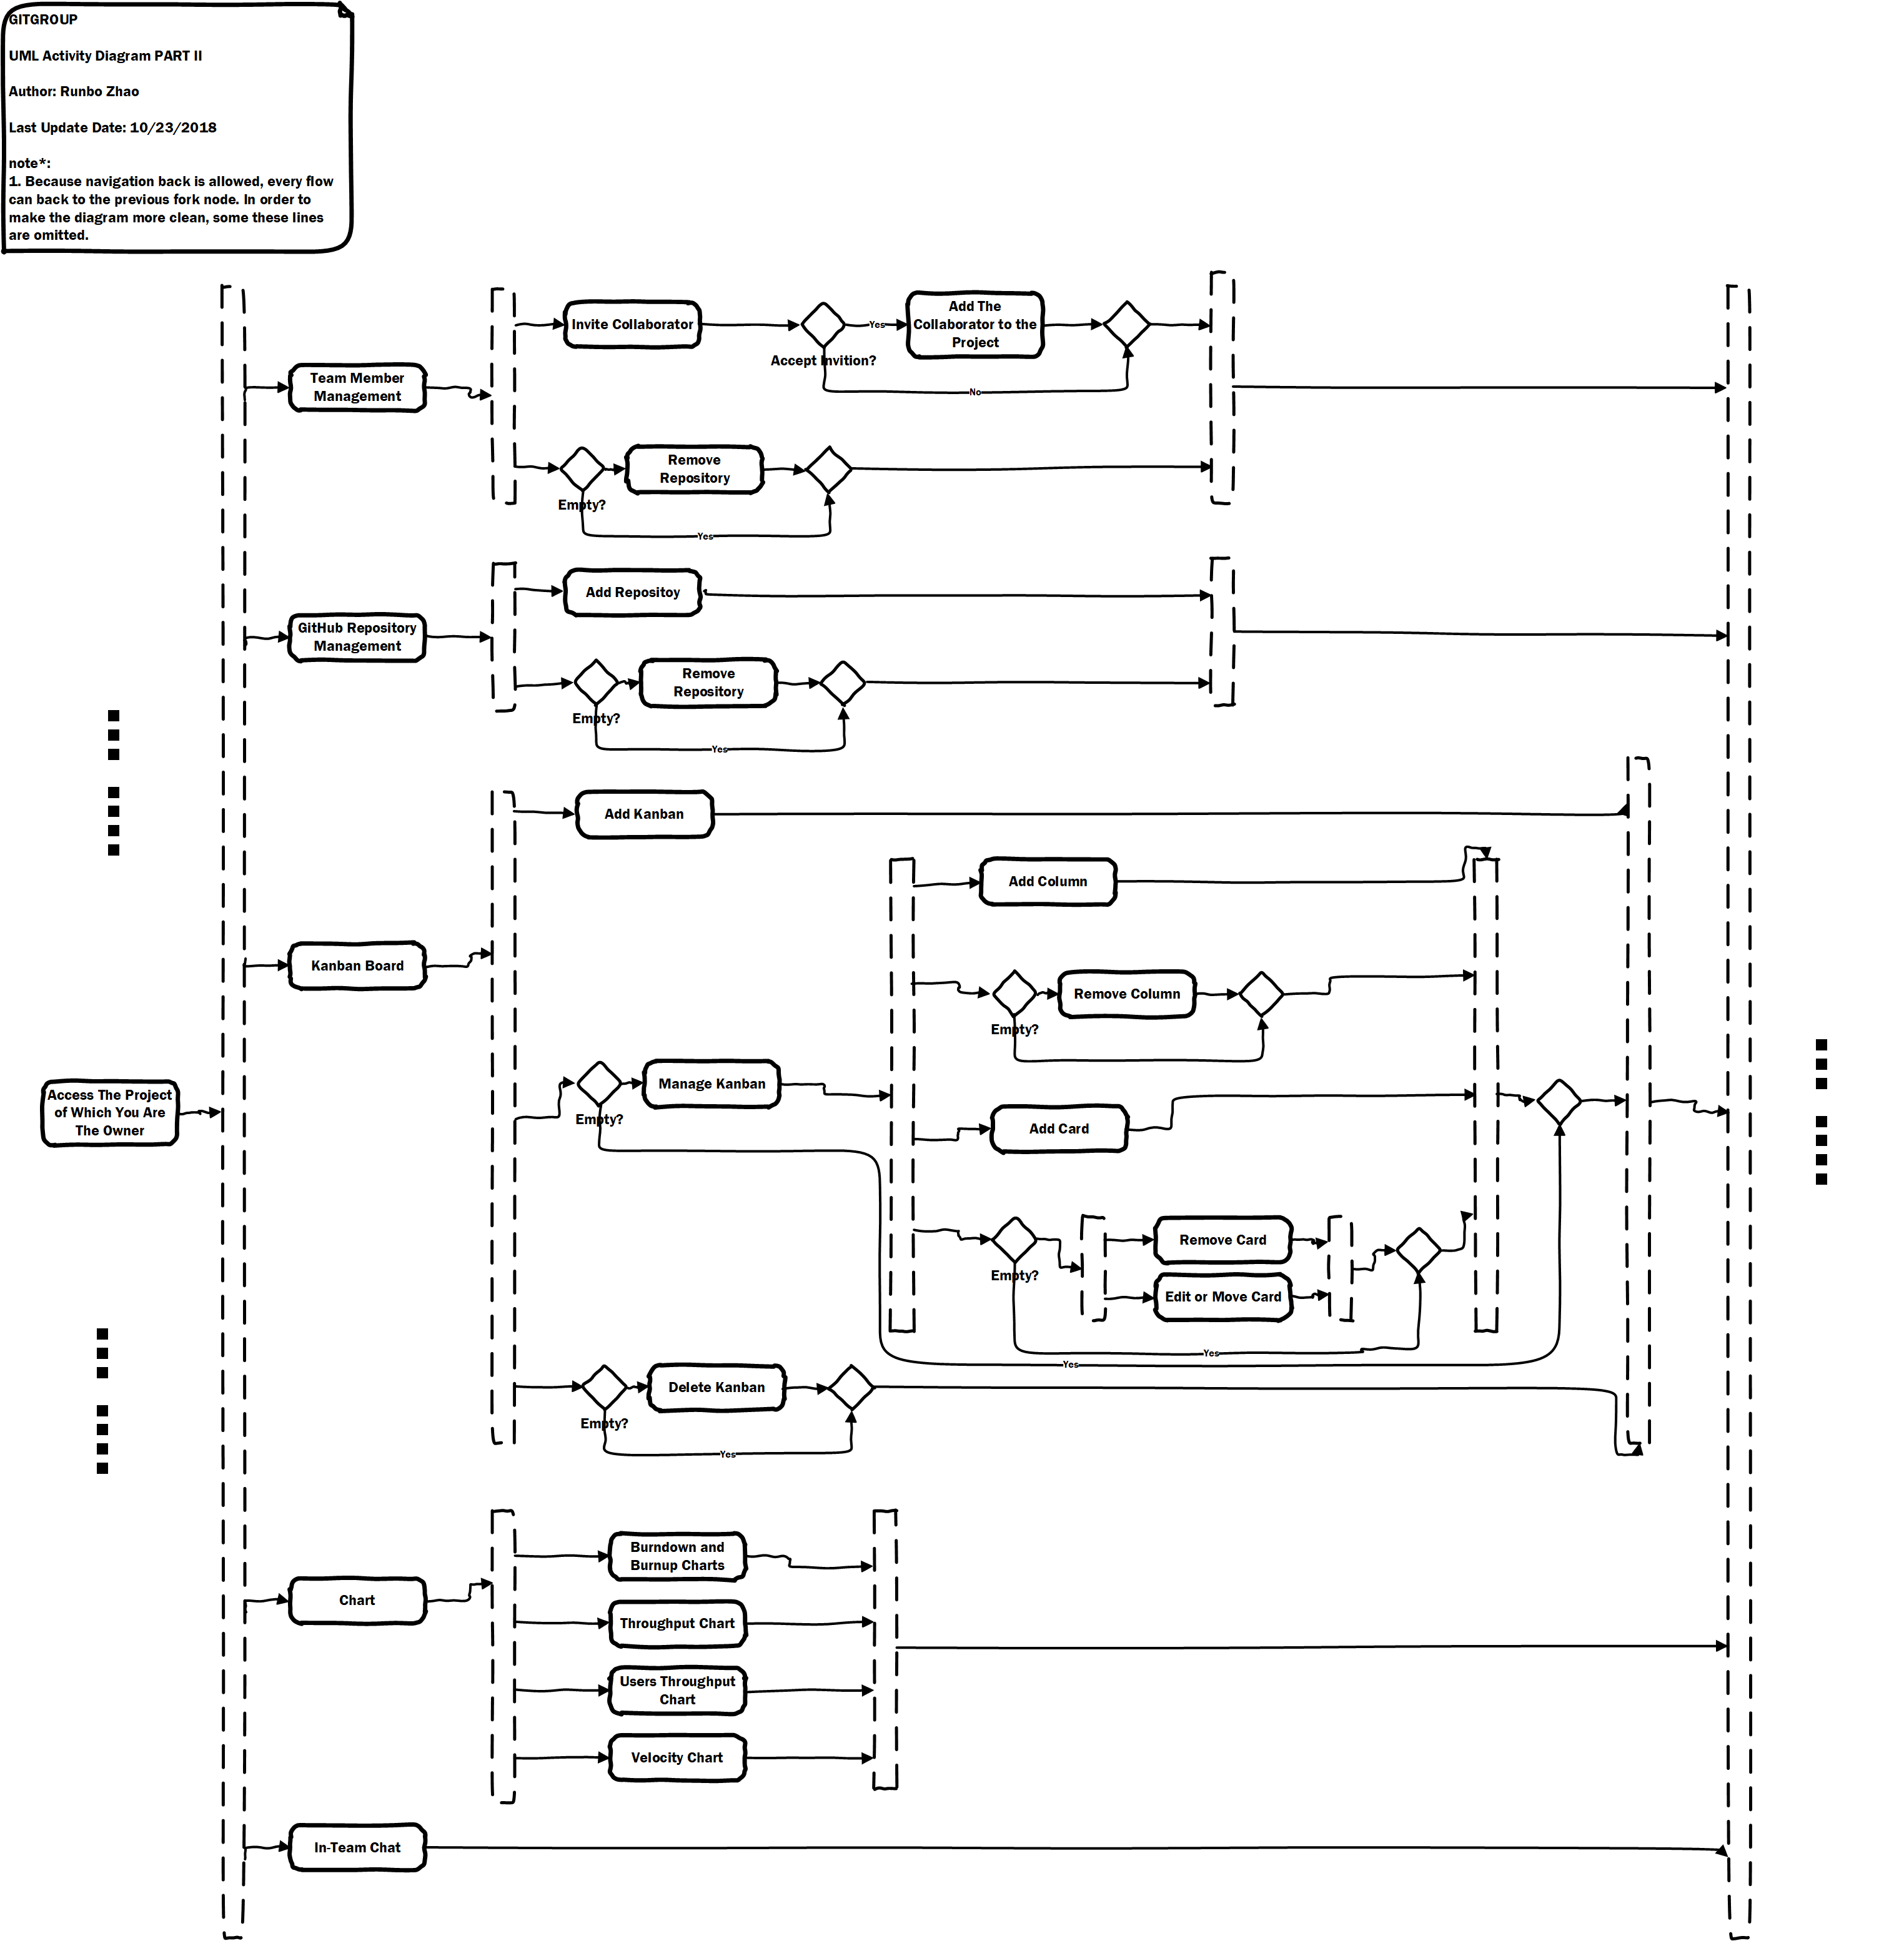
\includegraphics[width=0.7\textwidth]{./pics/ActivatyDiagramPARTII.png}
	\caption{Activity Diagram PART II (Details in Appendix A)}
\end{figure}
According to the activity diagram, the workflow of GitGroup is:\\
The user tries to log in and this generates an authentication request which uses GitHub to verify the identity of the user.
If it is an unregistered user, the user can sign up.\\
After successful login, the user is redirected to his/her dashboard. Here the user can manage their projects and team. The data is fetched from MongoDB.\\
The user has functionalities of creating a new project, removing a project after checking if it is empty.\\
After user creates a project, he/she has administration privilege of organizing a team to finish the software development, managing team members and GitHub repositories like adding or removing collaborators and repositories.\\
The major part of their dashboard is Kanban boar, which is a significant tool to help developer manage the development process. In the Kanban board, there are several columns represent different stage of the development process, such as TODO, Ready, In Progress, Done... \\
User can add or remove Kanban board and customize your own Kanban board column which can classify you cards of different development stage. Every column contains issue card imported from the GitHub, and you can easily drag them among the columns. If you drag it to the Done column. The issue in the GitHub will be automatically closed.  \\
The second part of dashboard is four charts, Burndown and Burnup charts, Throughput chart, Users Throughput chart and Velocity Chart, to analysis the development duration, quality and the team work situation of the project.\\
The communication among team members can also be done in the page of the GitGroup. Team member can easily chat with each other after integrating the chat room into GitGroup. The issue cards are easily transported among the team member through the chat system. Team owner can send notification of online meeting chat. User can also start a group chat in the global scope.\\
User also has functionalities of viewing and editing his/her profile.

\section{Sequence Diagram}
A sequence diagram shows object interactions arranged in time sequence. It depicts the objects and classes involved in the scenario and the sequence of messages exchanged between the objects needed to carry out the functionality of the scenario.
The following sequence diagram is used to show how GitHub authorization works.
\begin{figure}[H]
	\centering
	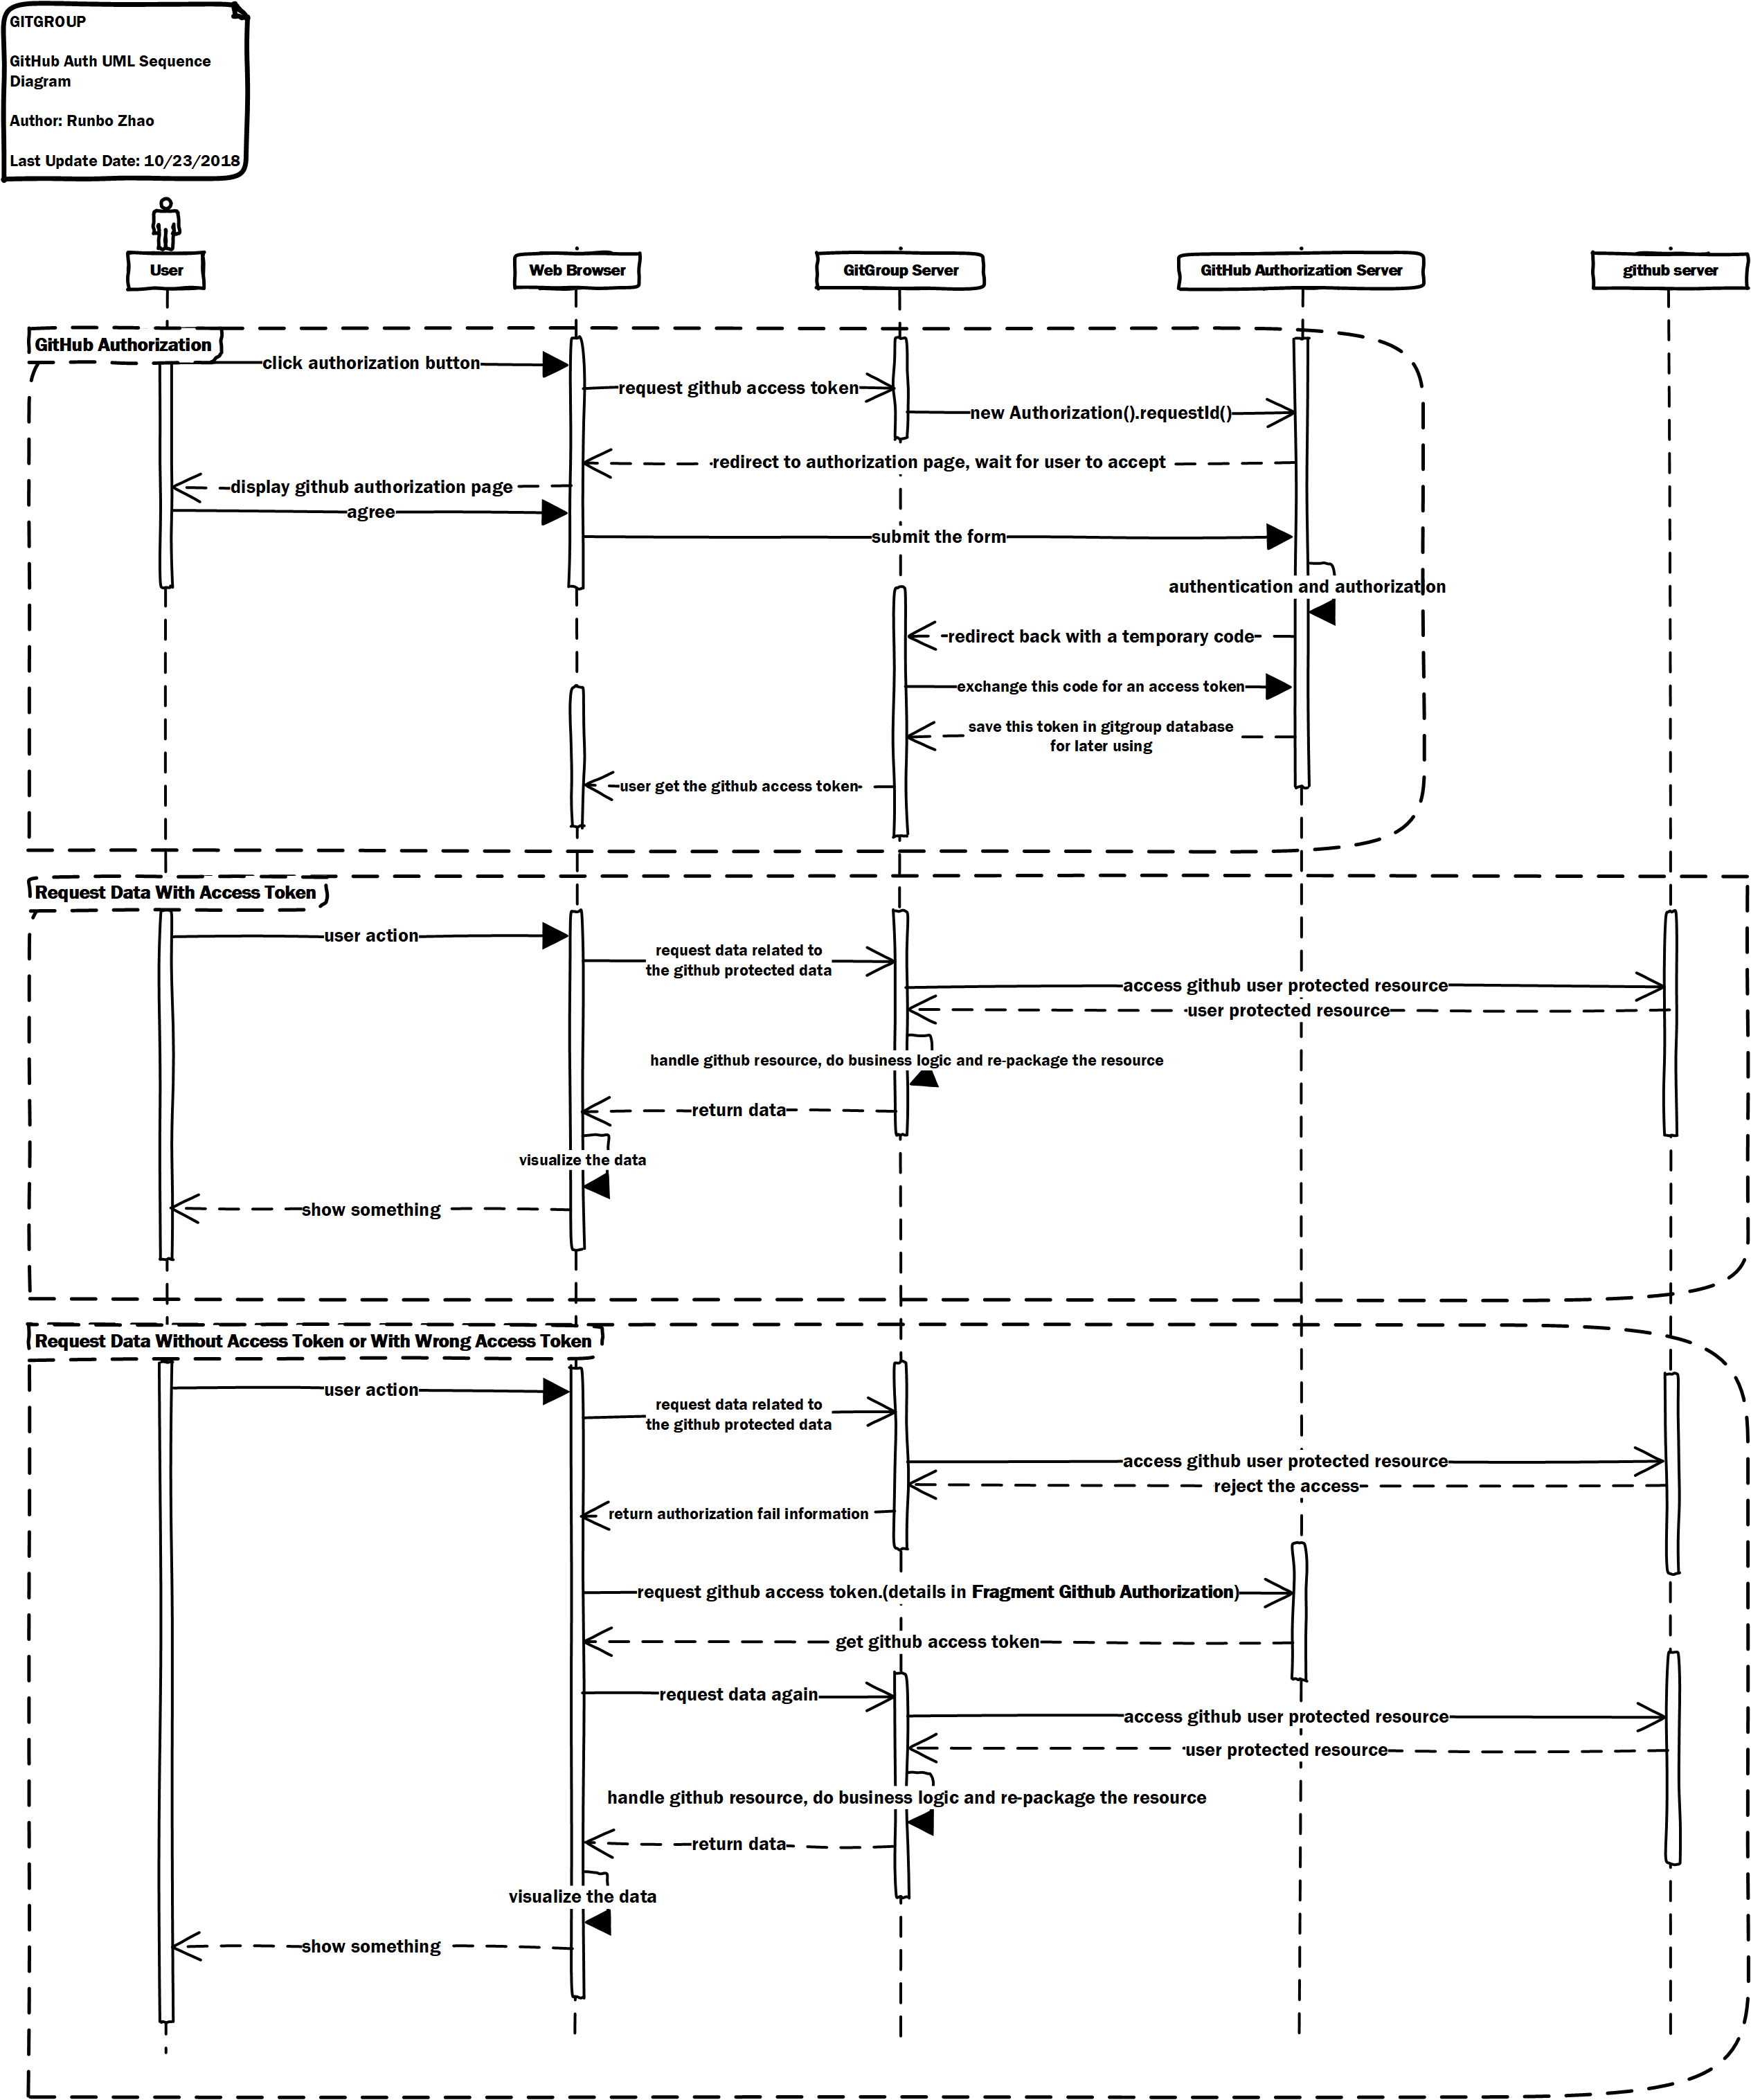
\includegraphics[width=0.7\textwidth]{./pics/AuthSequenceDiagram.png}
	\caption{Sequence Diagram For Authorization (Details in Appendix A)}
\end{figure}

GitGroup acts on behalf of a user, it performs user-to-server requests. These requests must be authorized with a user's access token. User-to-server requests include requesting data for a user, like determining which repositories to display to a particular user. These requests also include actions triggered by a user, like running a build, in order to identifying and authorizing users on GitGroup, it must identify GitHub users when they visit GitGroup using OAuth.\\
When GitGroup user click authorization button they are redirected to request his/her GitHub identity. The web browser will send a request for GitHub access token to GitGroup server, and GitGroup server redirected to request a GitHub identity to GitHub Authorization Server. \\
Then GitHub redirects back to GitGroup authorization page, wait for user to accept. After user accept the request, web server submit the agree form to GitHub authorization server, and GitHub redirects back with a temporary code in a code parameter as well as the state GitGroup server provided in the previous step in a state parameter. If the states don?t match, the request was created by a third party and the process should be aborted. GitGroup exchange this code for an access token, then save this token in GitGroup database for later using and user get the GitHub access token. \\
When user request data with access token, user are directed to request data related to the GitHub protected data, and GitGroup server request to access GitHub user protected resource and handle GitHub resource, do business logic and re-package the resource. At last GitGroup return data to web server, web server visualize the data and display it to user.\\
Once user request data without access token or with wrong access token which means GitGroup cannot access GitHub user protected resource. After GitHub reject the access, GitGroup server return authorization fail information to user. User will request data successfully only if user request correct GitHub access token.\\
\\
The following sequence diagram shows the how the 3 sub-system including project management system, project analytics system and chat system interact with each other.
\begin{figure}[H]
	\centering
	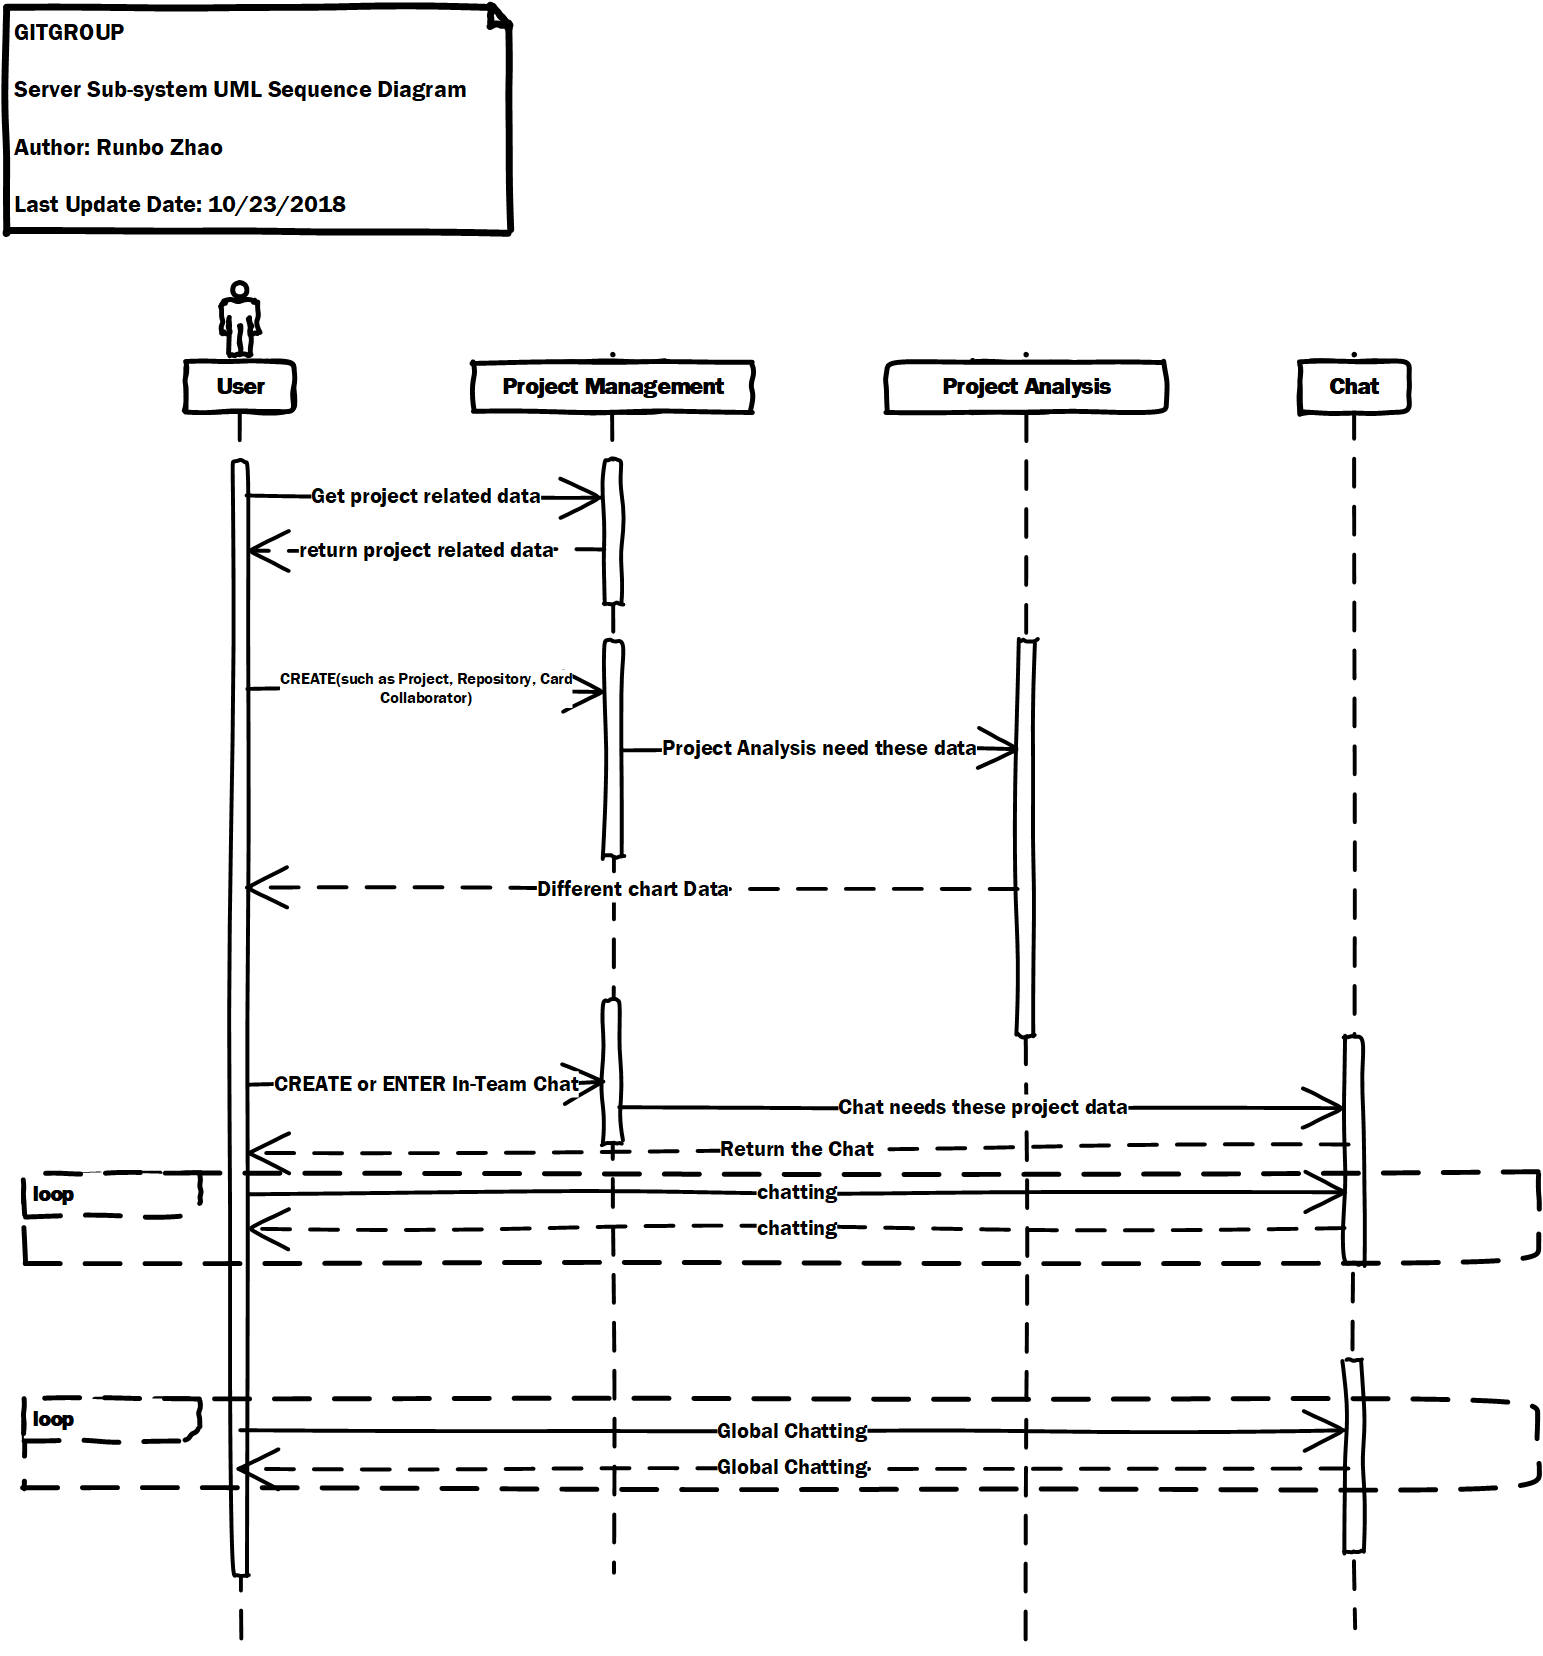
\includegraphics[width=0.7\textwidth]{./pics/SubSysSequenceDiagram.png}
	\caption{Sequence Diagram For Sub-Systems (Details in Appendix A)}
\end{figure}
Users can get and edit data via project management system. And the Project Analytics system must get data from project management system firstly and then return the analytics data to build chart. Also in-team chat need associate with project management system. But the global can work alone without any other systems.

\section{Class Diagram}
\begin{figure}[H]
	\centering
	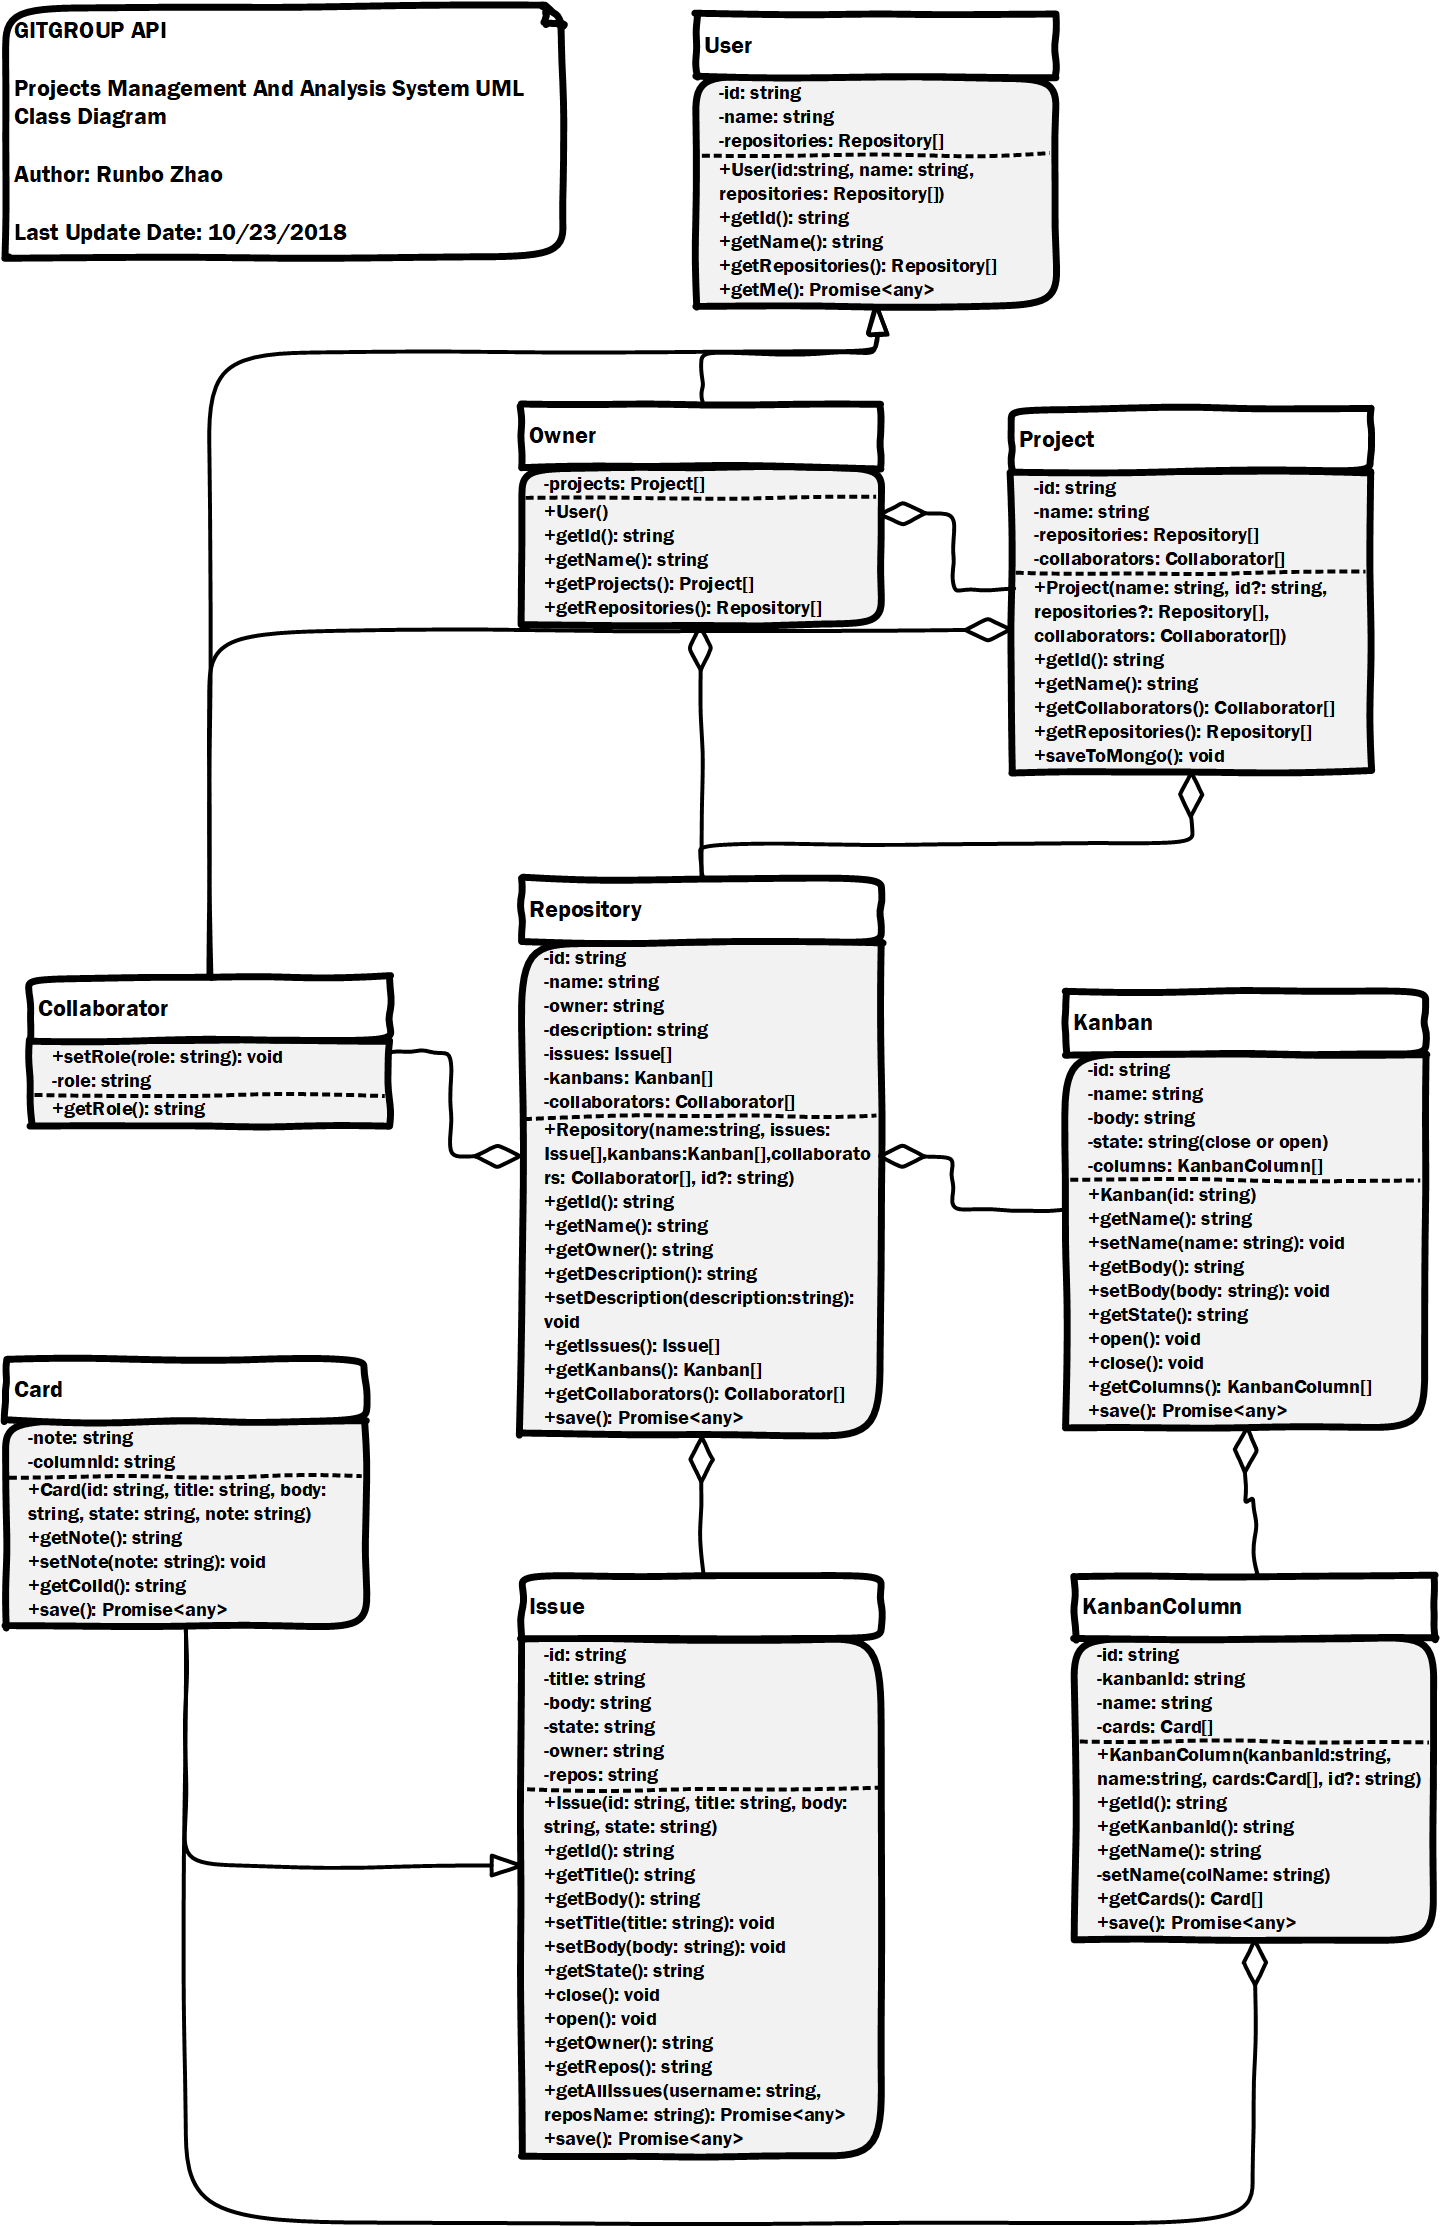
\includegraphics[width=0.6\textwidth]{./pics/ClassDiagram.png}
	\caption{UML Class Diagram (Details in Appendix A)}
\end{figure}
The project manage management system is the most important part of GitGroup.\\
User class represents the user of GitGroup, its properties are id, name and repositories. Because there are two types of users, there are two class Owner and Collaborator extend from User.\\
Project class represents the project in GitGroup, the project is the combination of repositories. Its properties have id, name, repositories and collaborators.\\
Repository class represents the repository in GitHub. Its properties have id, name, owner, description, issues, kanbans and collaborators. And also the Issue class represents the issue in GitHub.\\
KanBan, KanBanColumn and Card class are key classes for KanBan board functionality. Card's properties are note and the column id it belongs to. KanBan's properties are id, name, body, state(close or open) and columns it has. KanBanColumn's properties are id, name, KanBan which the column belong to, Cards which the column has.

% ----------------------------------------------
% Chapter 6 System Architecture
% ----------------------------------------------
\chapter{System Architecture}
\begin{figure}[H]
	\centering
	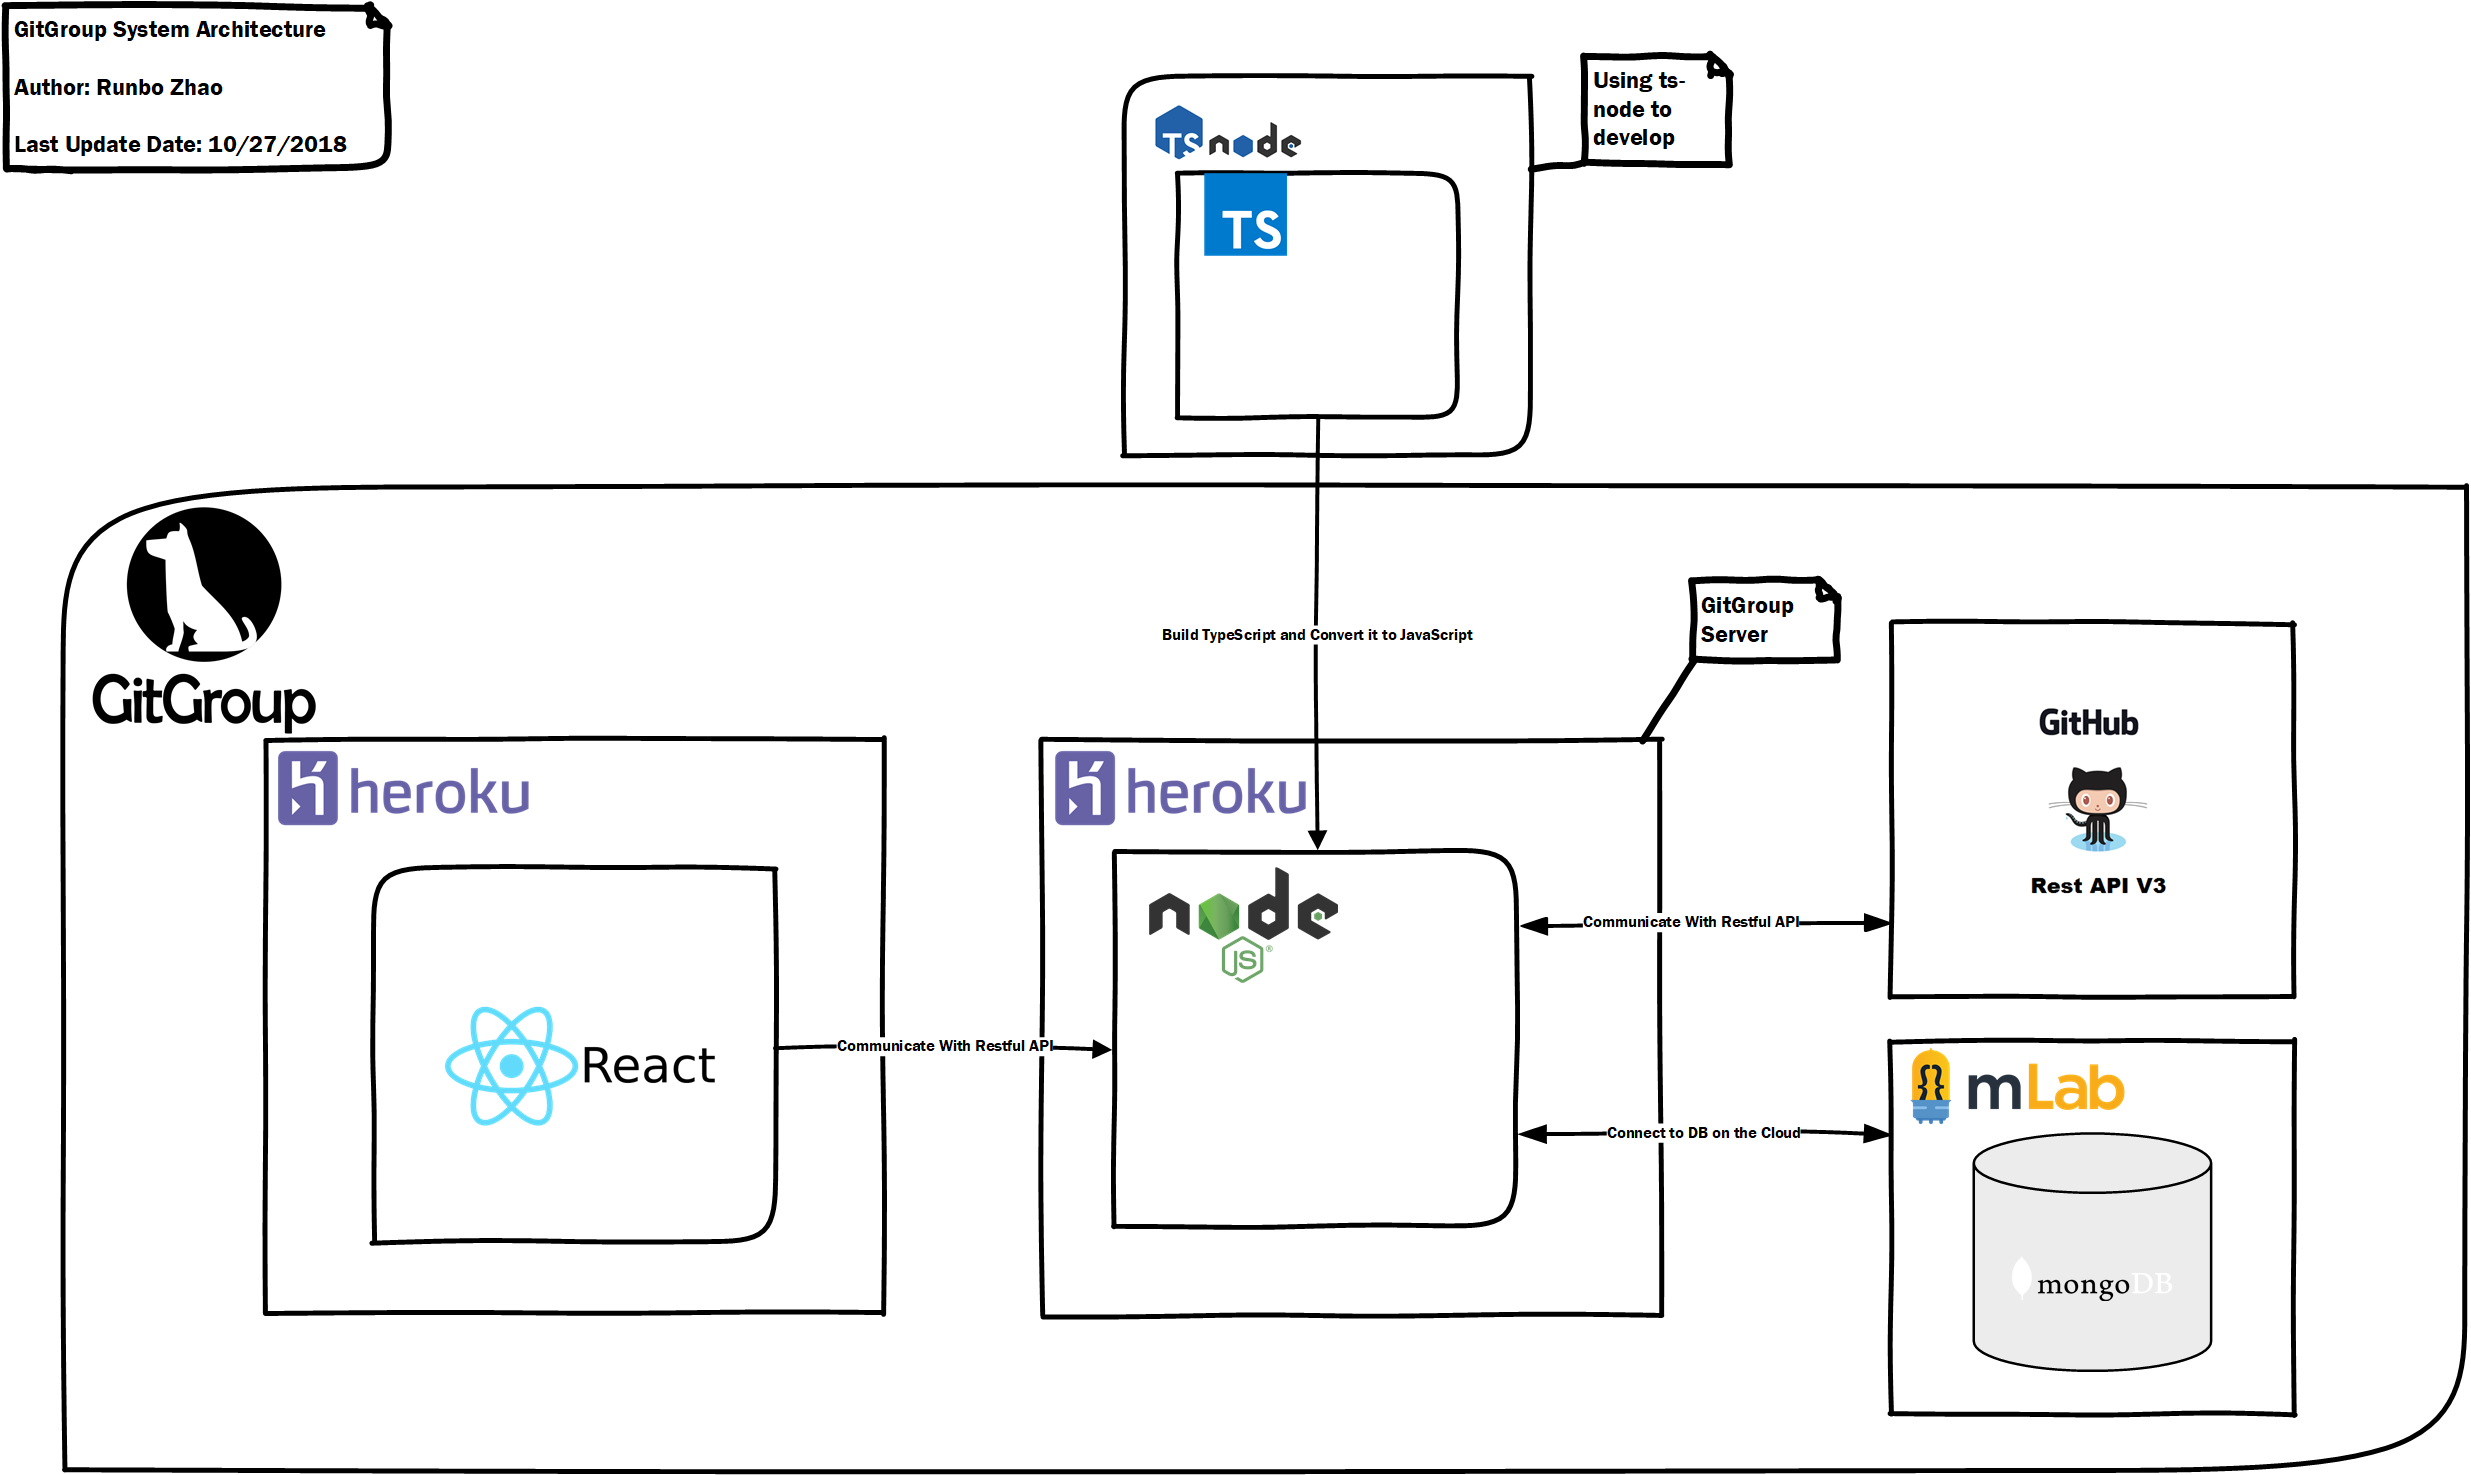
\includegraphics[width=0.9\textwidth]{./pics/SystemArchitecture.png}
	\caption{GitGroup System Architecture}
\end{figure}
\section{TypeScript}
TypeScript is an open-source programming language developed and maintained by Microsoft. It is a strict syntactical superset of JavaScript, and adds optional static typing to the language. \\
TypeScript is used to develop GitGroup because its strong Object-Oriented-Programming features.\\
TypeScript is designed for development of large applications and transcompiles to JavaScript.As TypeScript is a superset of JavaScript, existing JavaScript programs are also valid TypeScript programs. TypeScript may be used to develop JavaScript applications for both client-side and server-side (Node.js) execution.\\
\section{mLab}
mLab is a fully managed cloud database service that hosts MongoDB databases. mLab runs on cloud providers Amazon, Google, and Microsoft Azure, and has partnered with platform-as-a-service providers. 
\section{MongoDB}
MongoDB is a free and open-source cross-platform document-oriented database program. Classified as a NoSQL database program, MongoDB uses JSON-like documents with schemata. MongoDB is developed by MongoDB Inc., and is published under a combination of the Server Side Public License and the Apache License. 
\\
MongoDB is used via mLab in this project. And Mongoose is chosen as the ORM(Object-relational mapping).
\section{Express}
Express, a web server built on Node.js, forms the middle tier or the web server. It defines routes, specifications of what to do when a HTTP request matching a certain pattern arrives. The matching specification is regular expression (regex) based and is very flexible. The what-to-do part is just a function that is given the parsed HTTP request. Express parses request URL, headers, and parameters for us. On the response side, it has, as expected, all of the functionality required by web applications including setting response codes, setting cookies, sending custom headers, etc.  
\section{React}
React is a front-end technology from Facebook. It?s not a full-fledged MVC framework, but it?s a JavaScript library for building user interfaces, so in some sense it?s the view part of MVC. We use React to render a view because it tries to solve the problem from the View layer by creating abstract representations of views. It breaks down parts of the view in the Components. These components encompass both the logic to handle the display of view and the view itself. It can contain data that it uses to render the state of the app. 
\section{NodeJs}
NodeJs, a server-side JavaScript runtime environment, has an asynchronous eventdriven, non-blocking input/output (I/O) model, as opposed to using threads to achieve multitasking. It relies heavily on callbacks and promises to let you know that a pending task is completed. Node.js achieves multitasking using an event-loop. This is nothing but a queue of events that need to be processed and callbacks to be run on those events. An event-based approach also makes Node.js applications fast and lets the programmer be blissfully oblivious of the semaphores and locks that are utilized to synchronize multithreaded events.  
\section{Heroku}
Heroku is a cloud platform as a service (PaaS) supporting several programming languages. Heroku, one of the first cloud platforms, has been in development since June 2007, when it supported only the Ruby programming language, but now supports Java, Node.js, Scala, Clojure, Python, PHP, and Go.\\
In this project, Heroku is the platform where GitGroup is deployed to.



% ----------------------------------------------
% Appendix
% ----------------------------------------------
\cleardoublepage
\appendix
\chapter{Figures}% <-- this title should appear on page header
\newgeometry{margin=1cm,includefoot}

\begin{figure}[h]
	\centering
	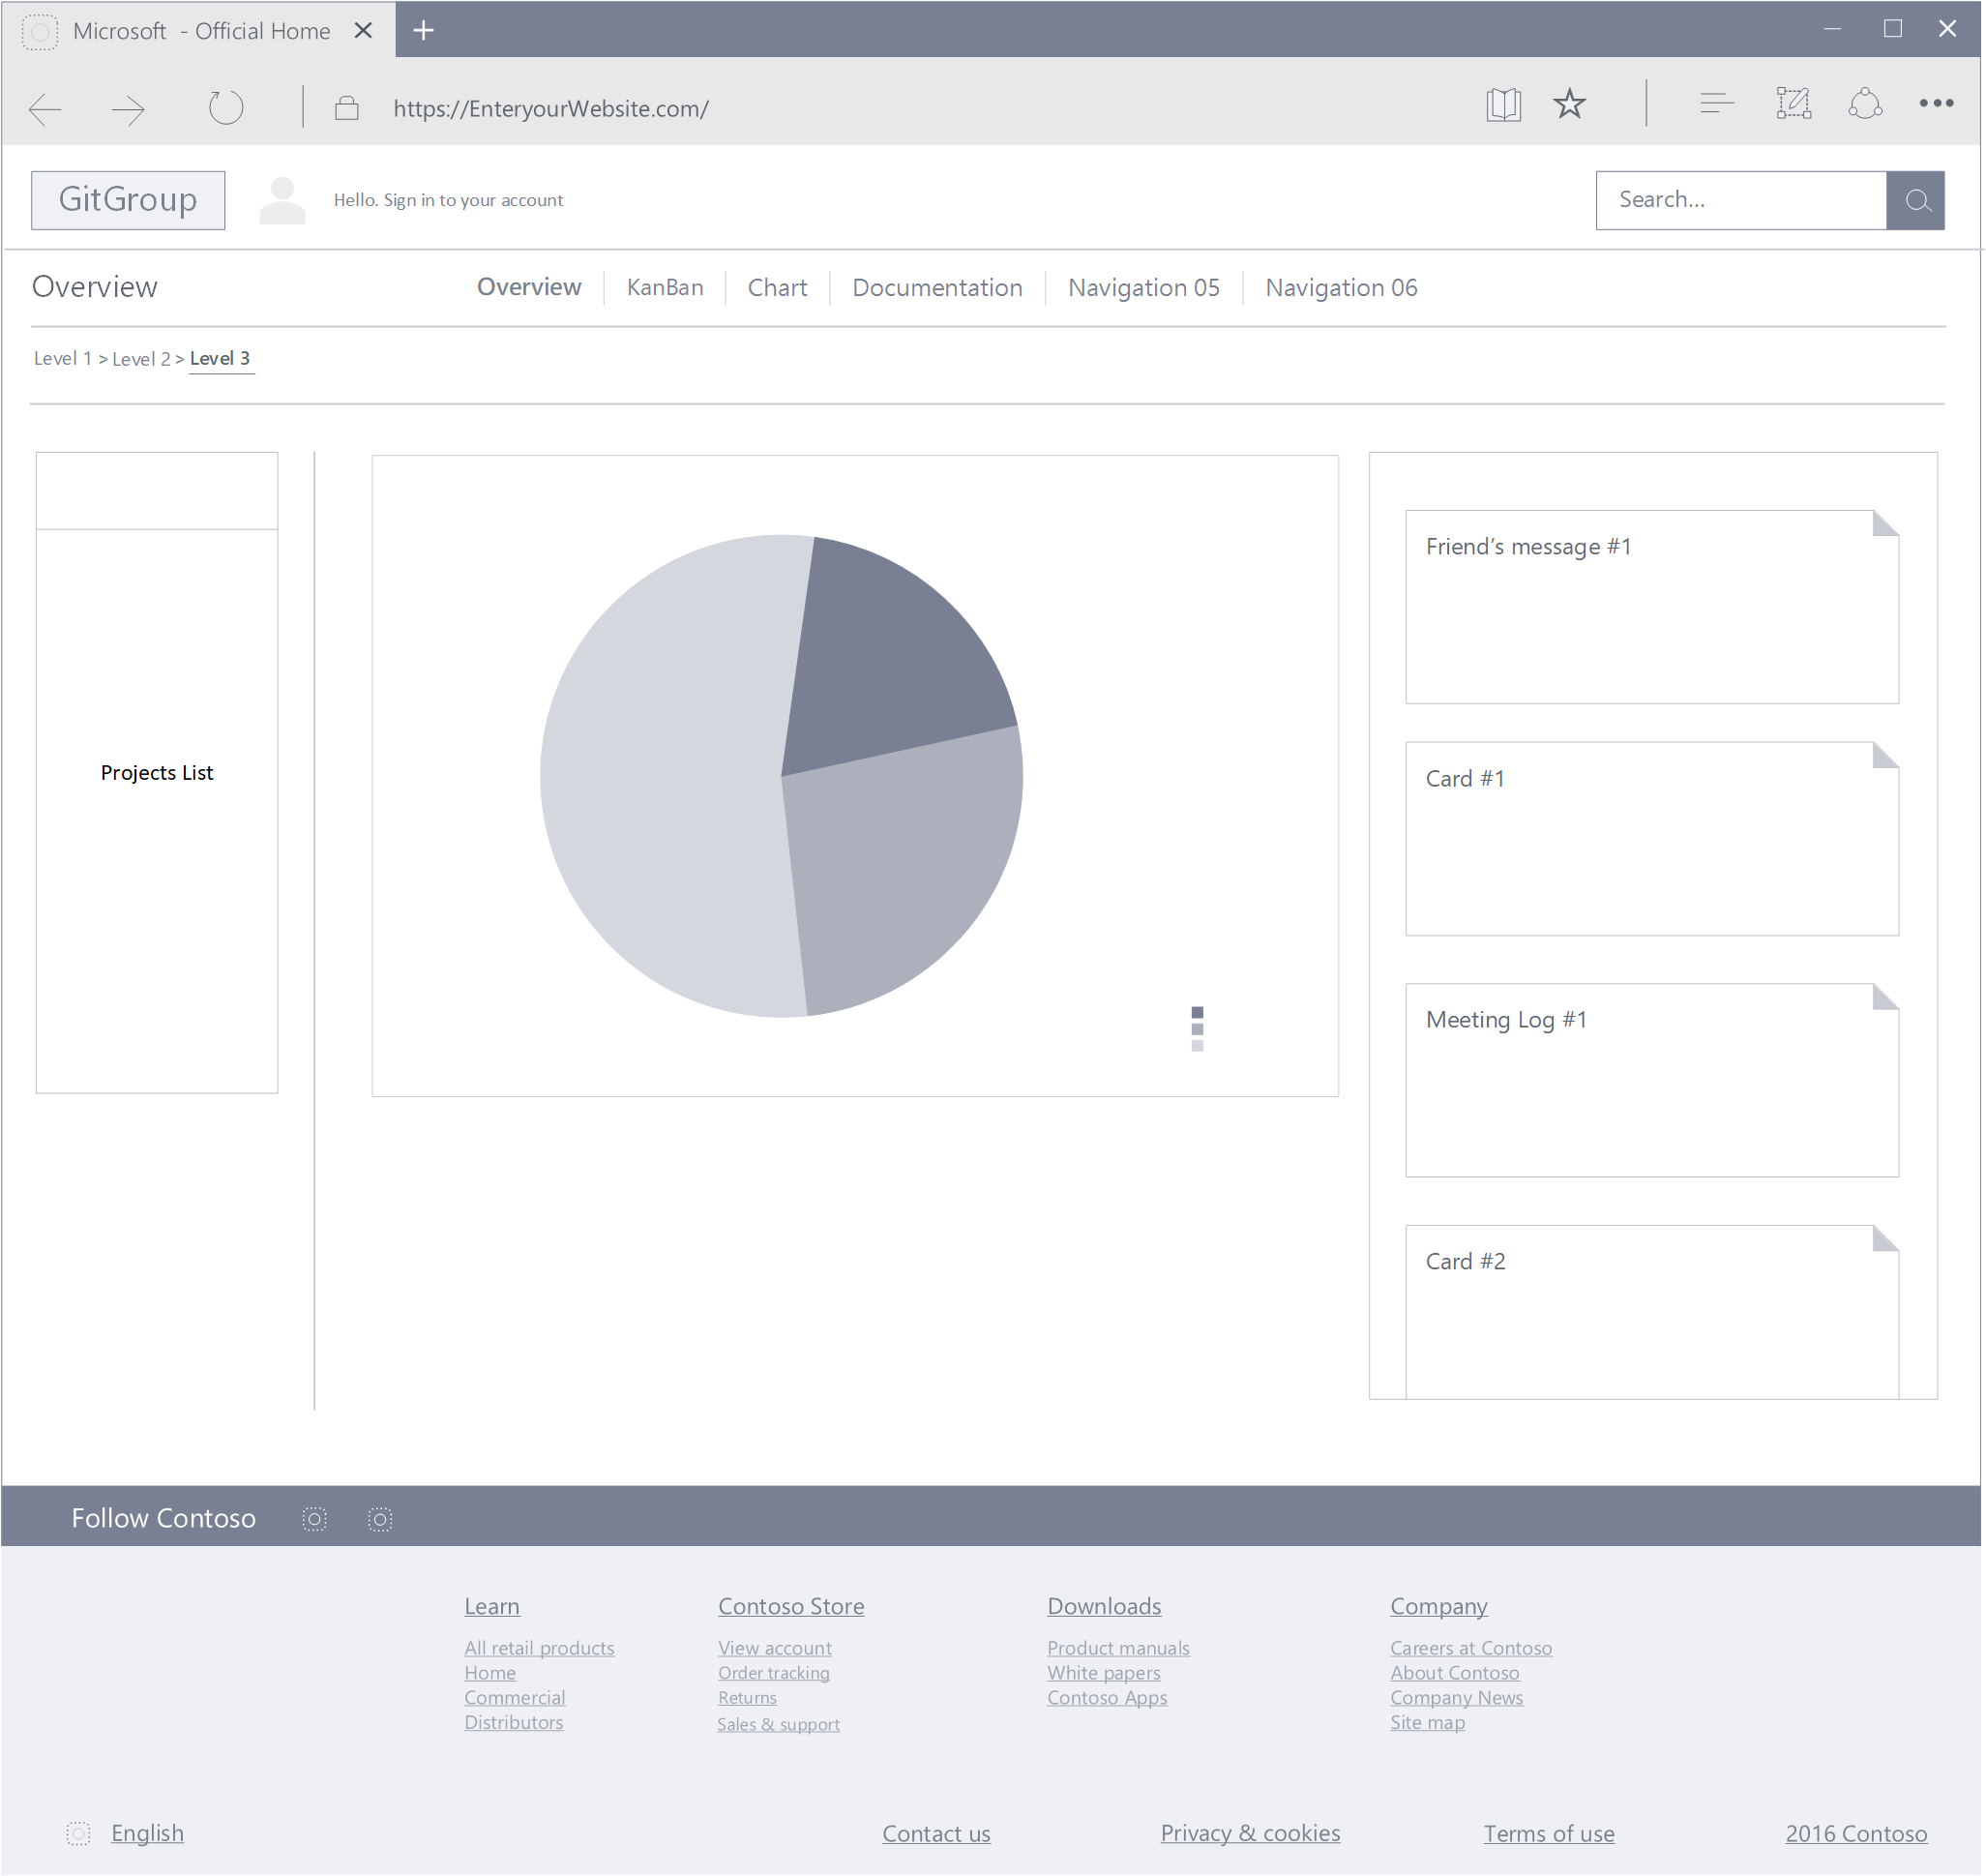
\includegraphics[width=\textwidth]{./pics/OverviewInterface.png}
	\caption{\textbf{DETAIL} Overview User Interface}
\end{figure}

\begin{figure}[h]
	\centering
	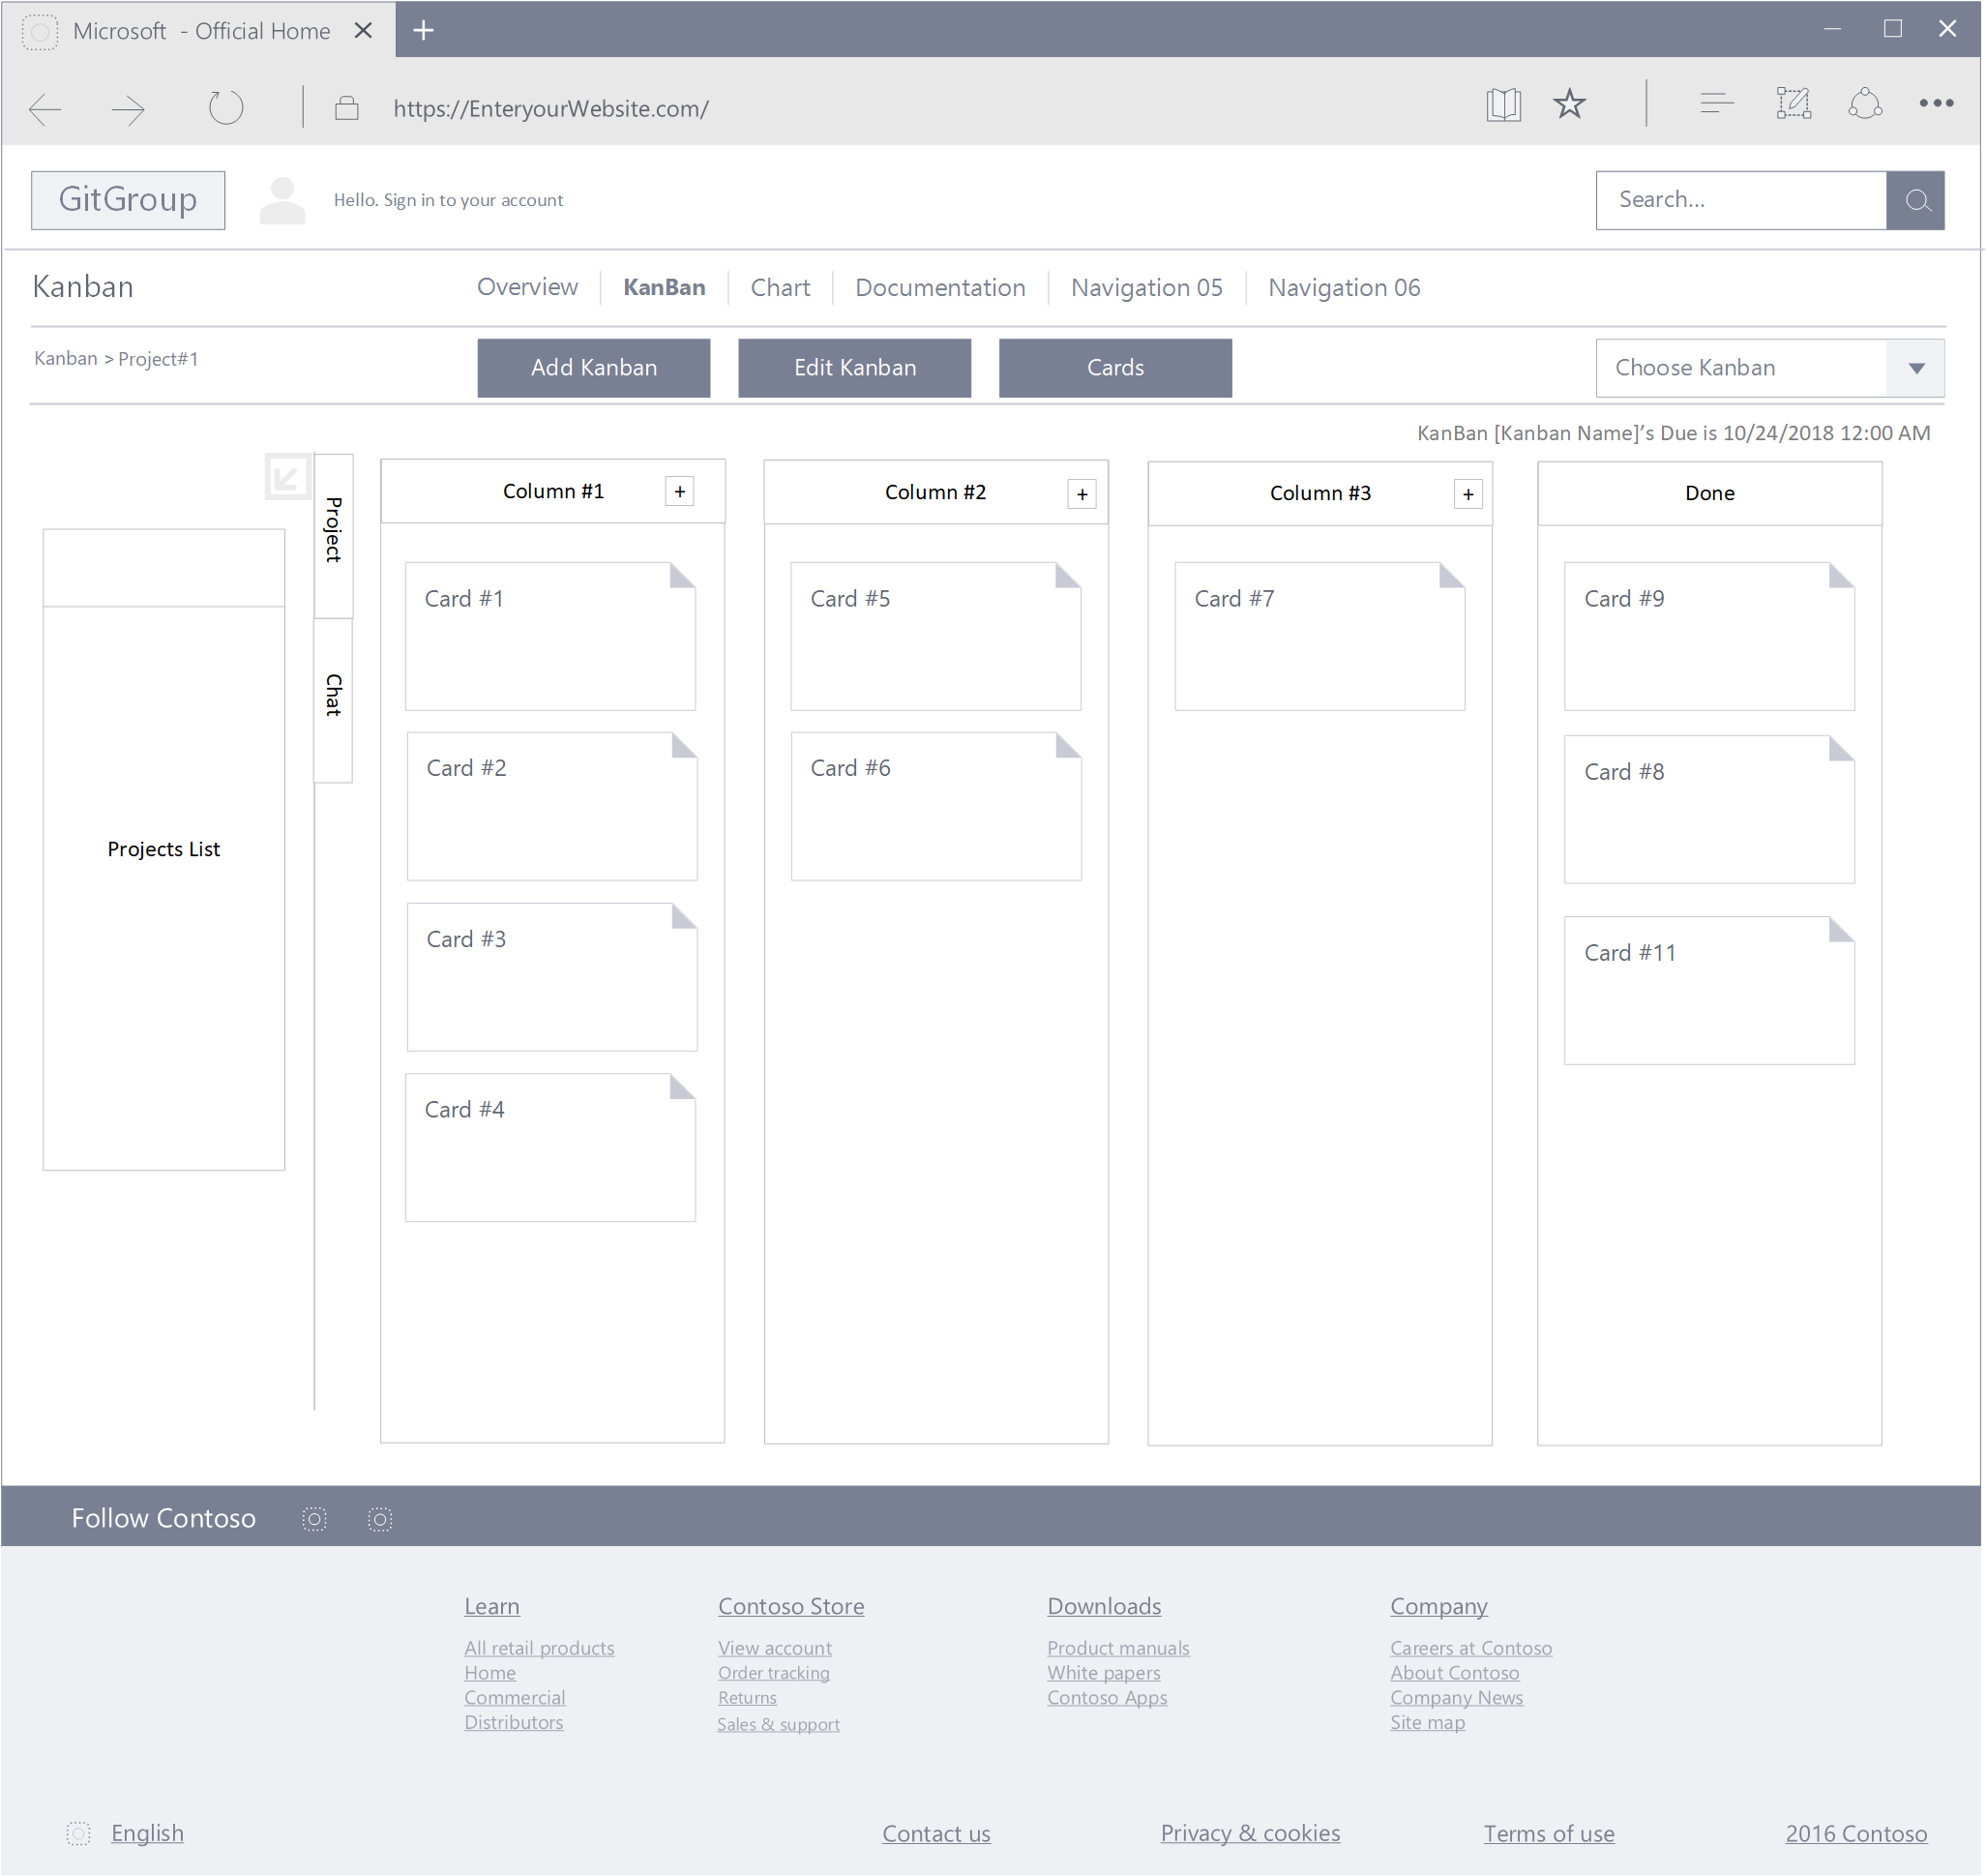
\includegraphics[width=\textwidth]{./pics/KanbanInterface.png}
	\caption{\textbf{DETAIL} KanBan User Interface}
\end{figure}

\begin{figure}[h]
	\centering
	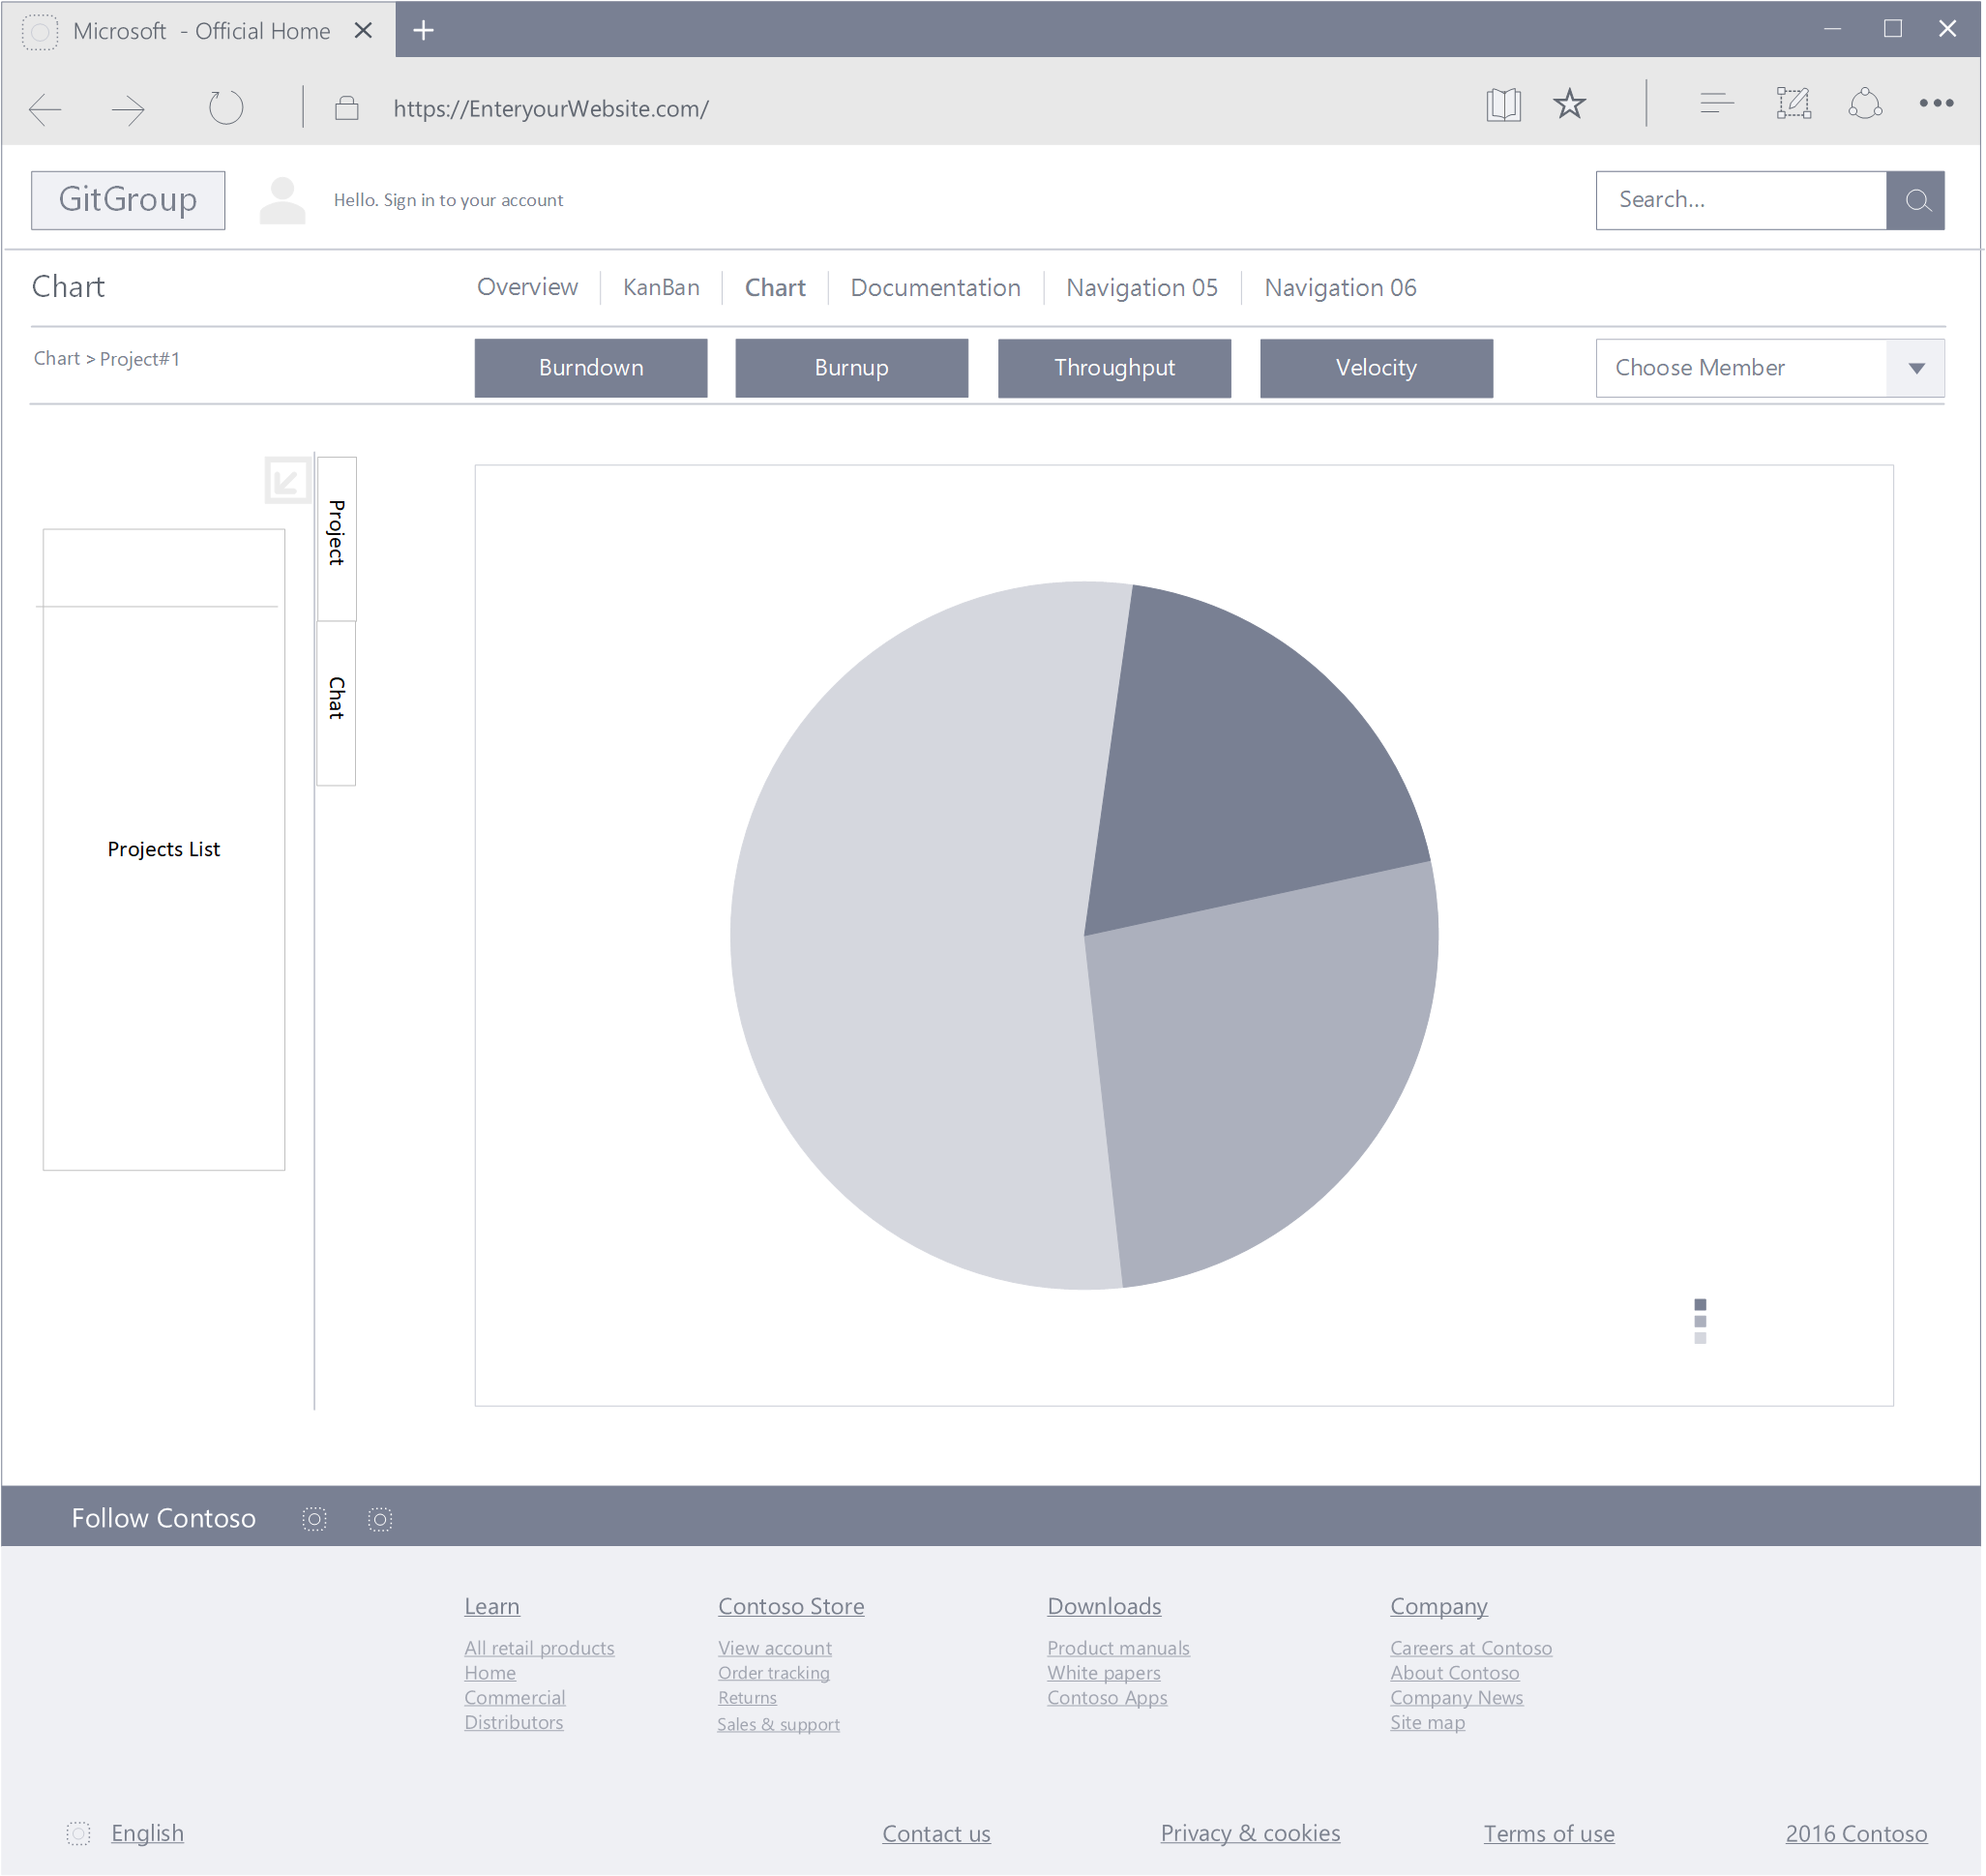
\includegraphics[width=\textwidth]{./pics/ChartInterface.png}
	\caption{\textbf{DETAIL} Chart User Interface}
\end{figure}

\begin{figure}[h]
	\centering
	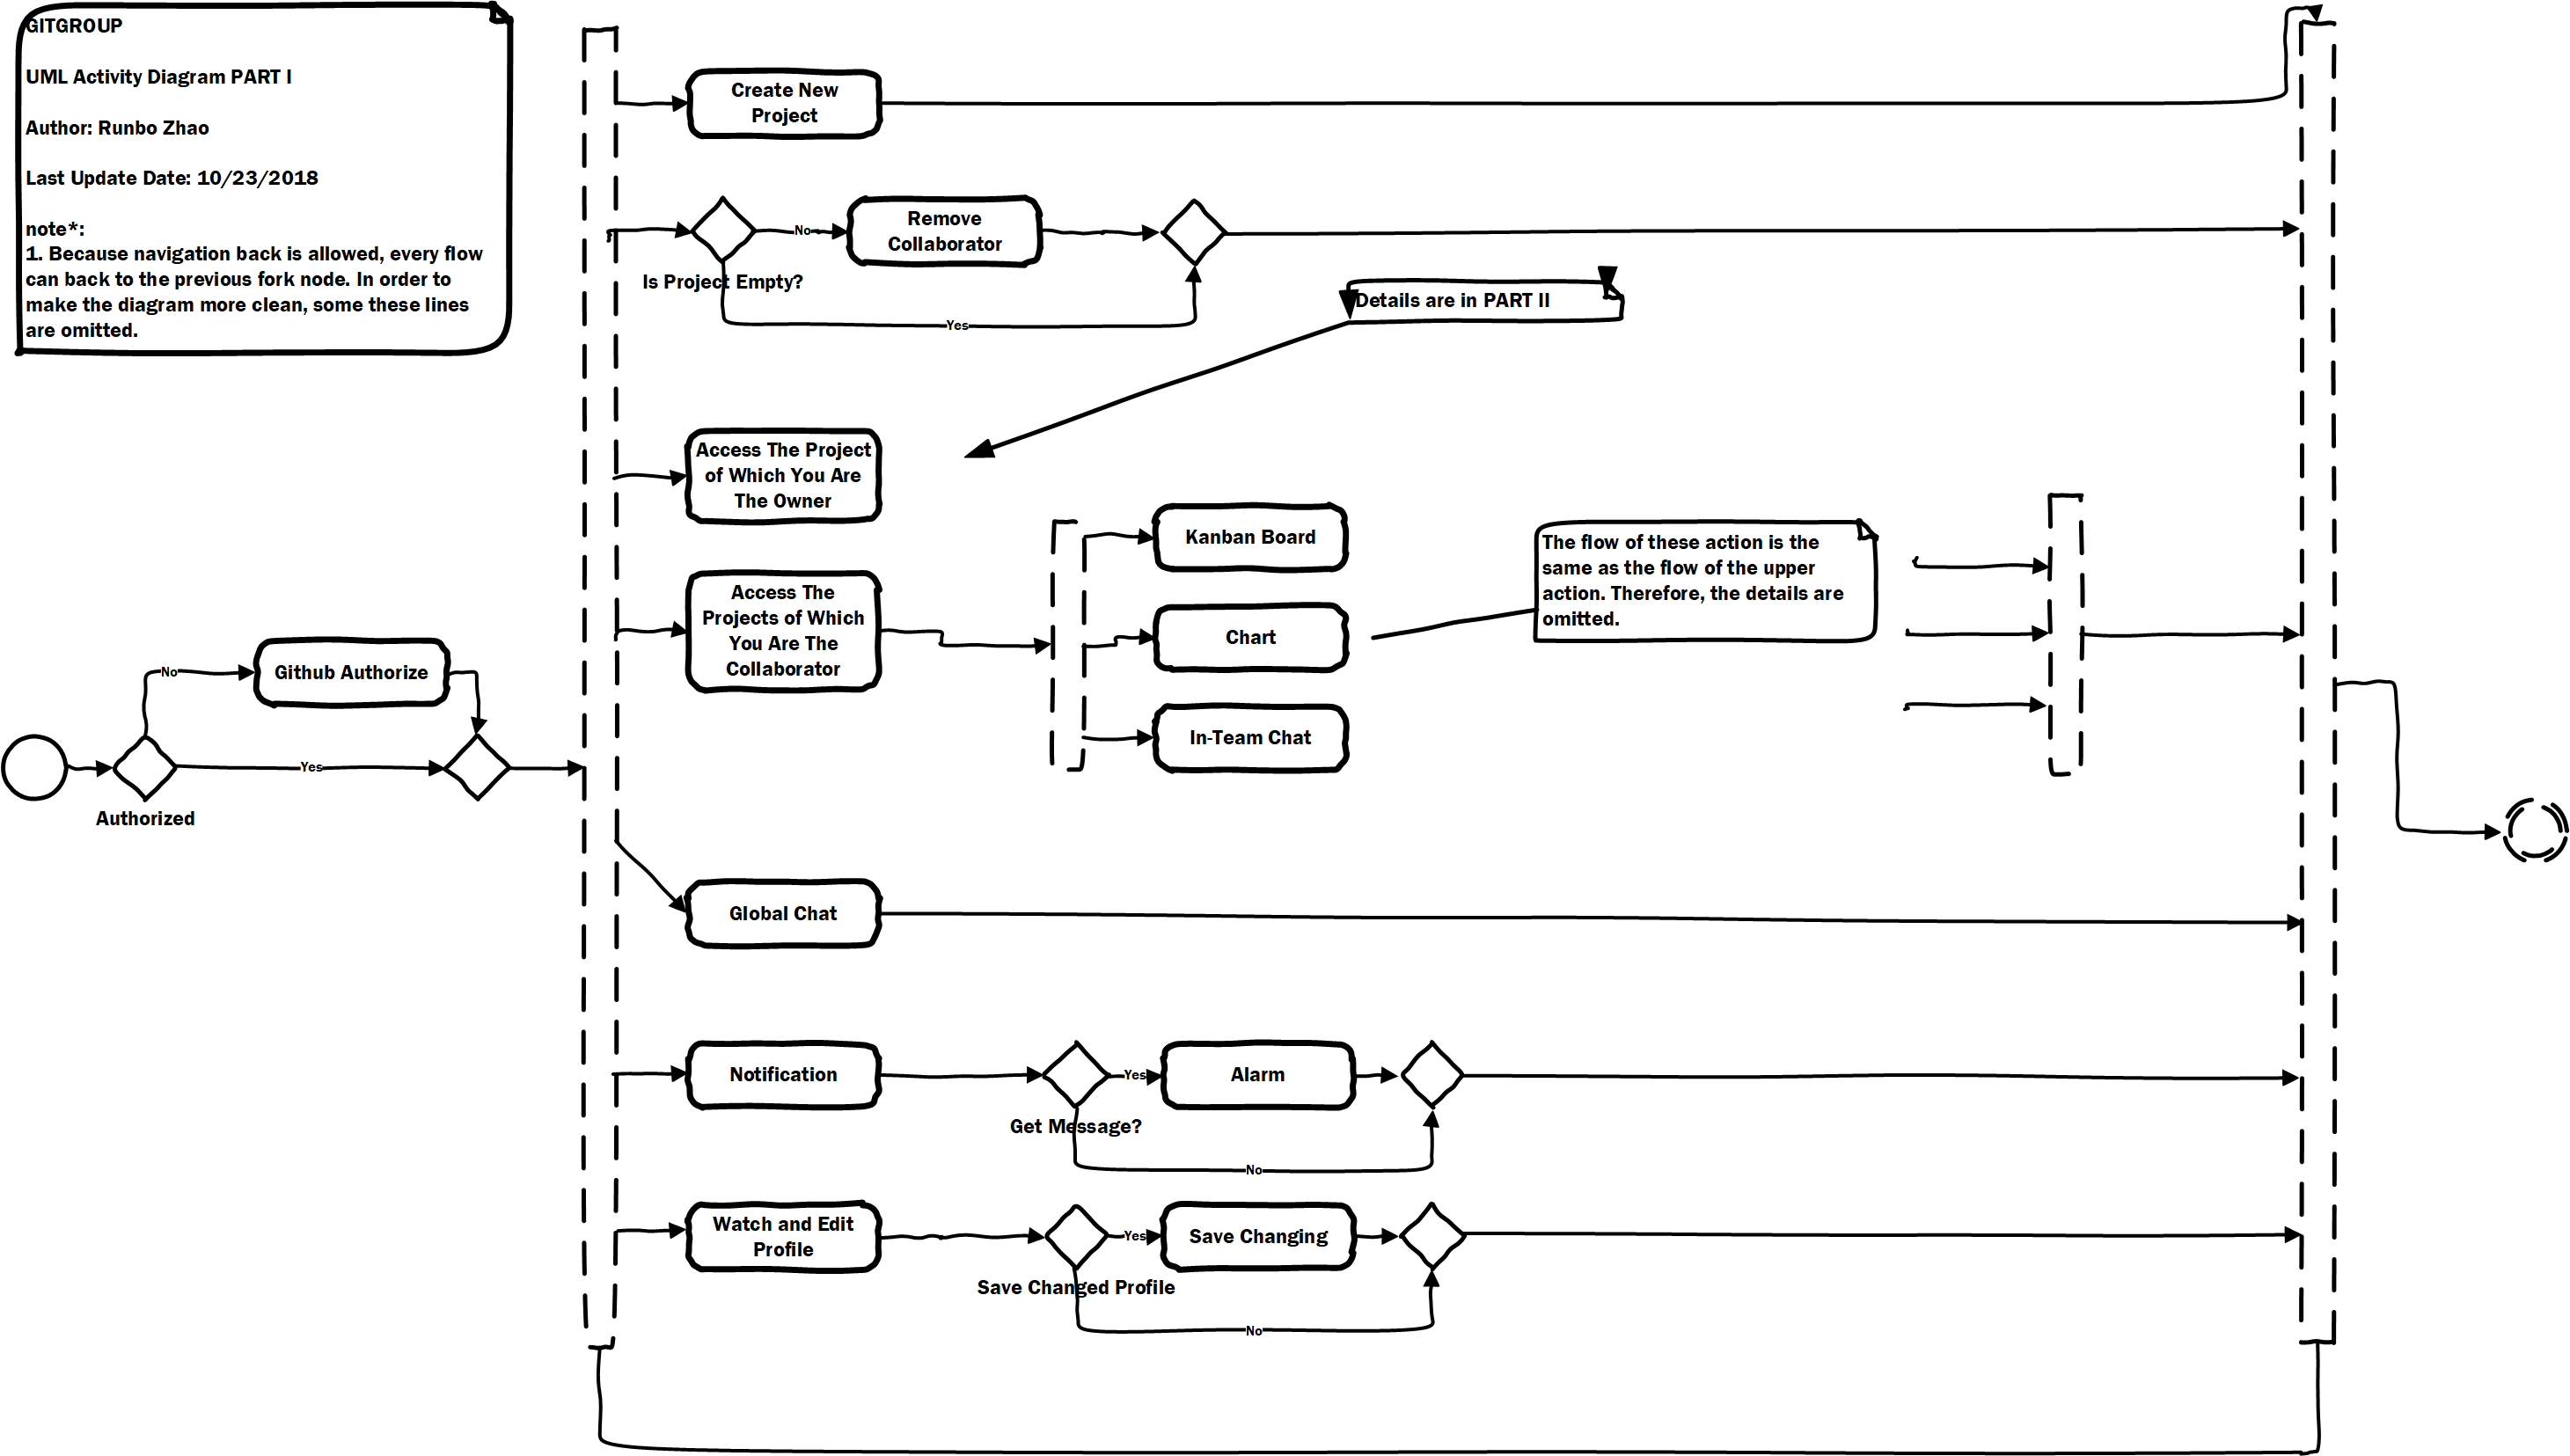
\includegraphics[scale=0.5,angle=90]{./pics/ActivatyDiagramPARTI.png}
	\caption{\textbf{DETAIL} Activity Diagram PART I}
	\label{fig1}
\end{figure}

\begin{figure}[h]
	\centering
	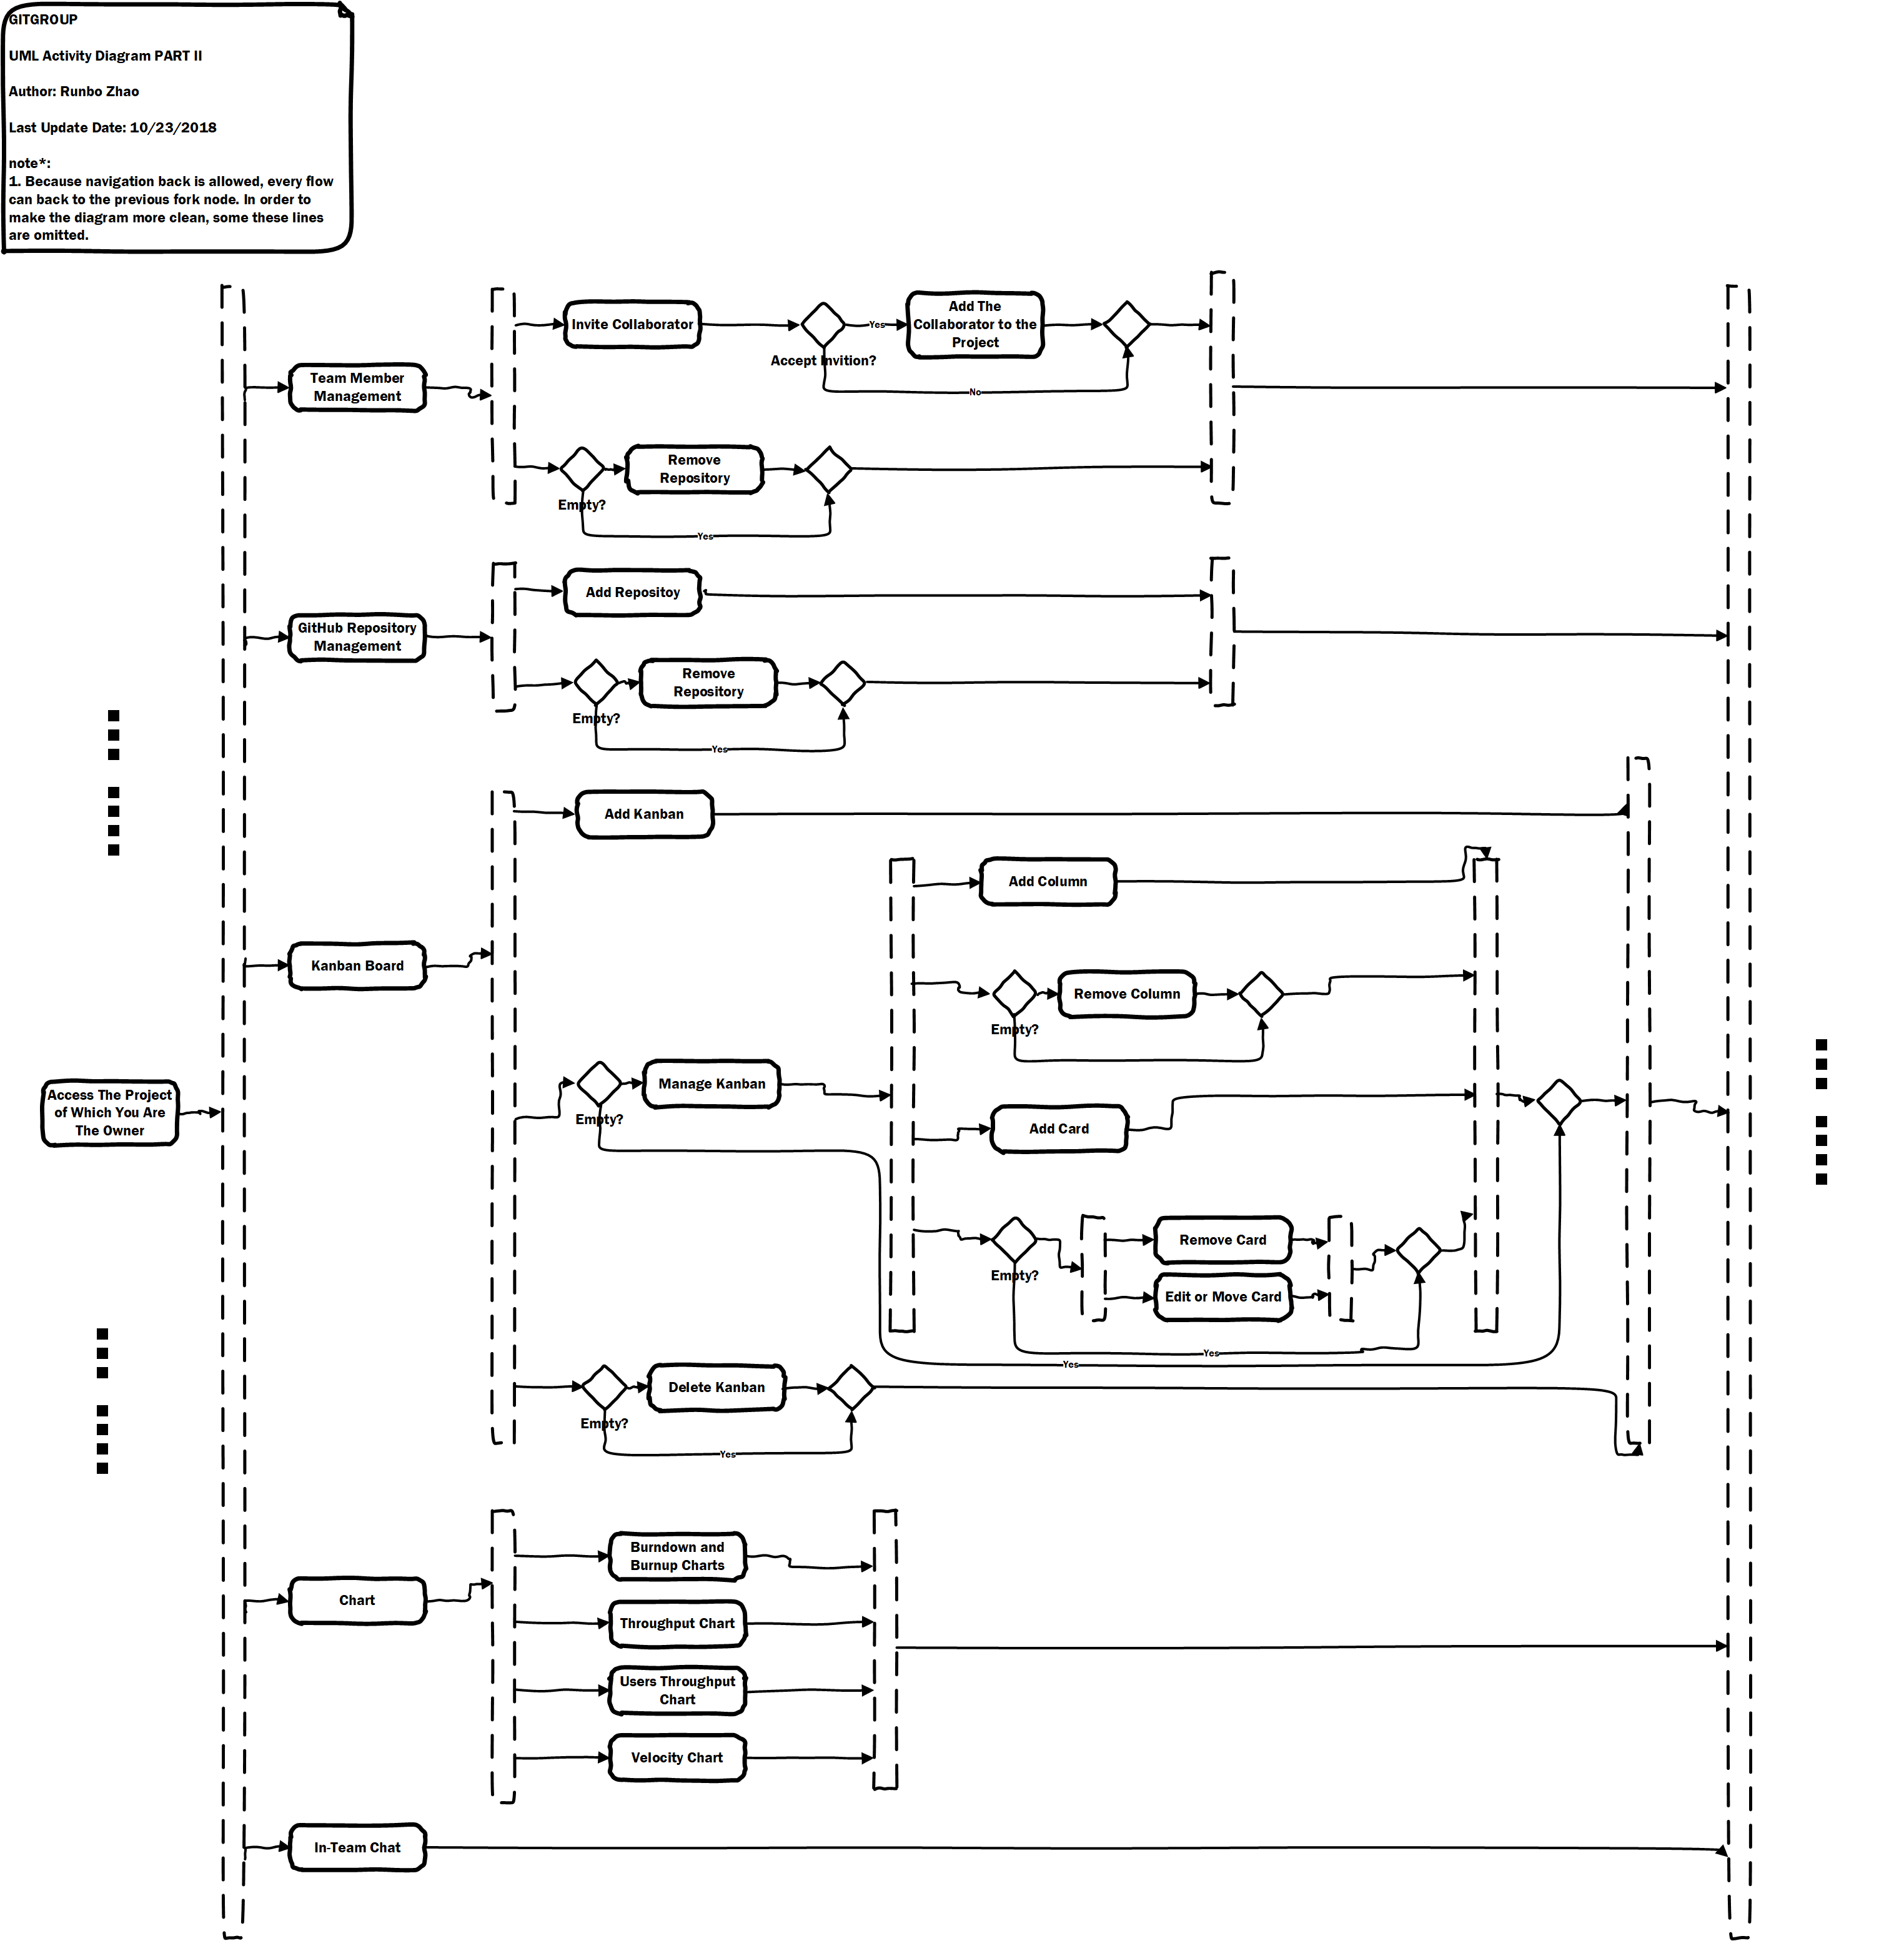
\includegraphics[width=\textwidth]{./pics/ActivatyDiagramPARTII.png}
	\caption{\textbf{DETAIL} Activity Diagram PART II}
	\label{fig2}
\end{figure}

\begin{figure}[h]
	\centering
	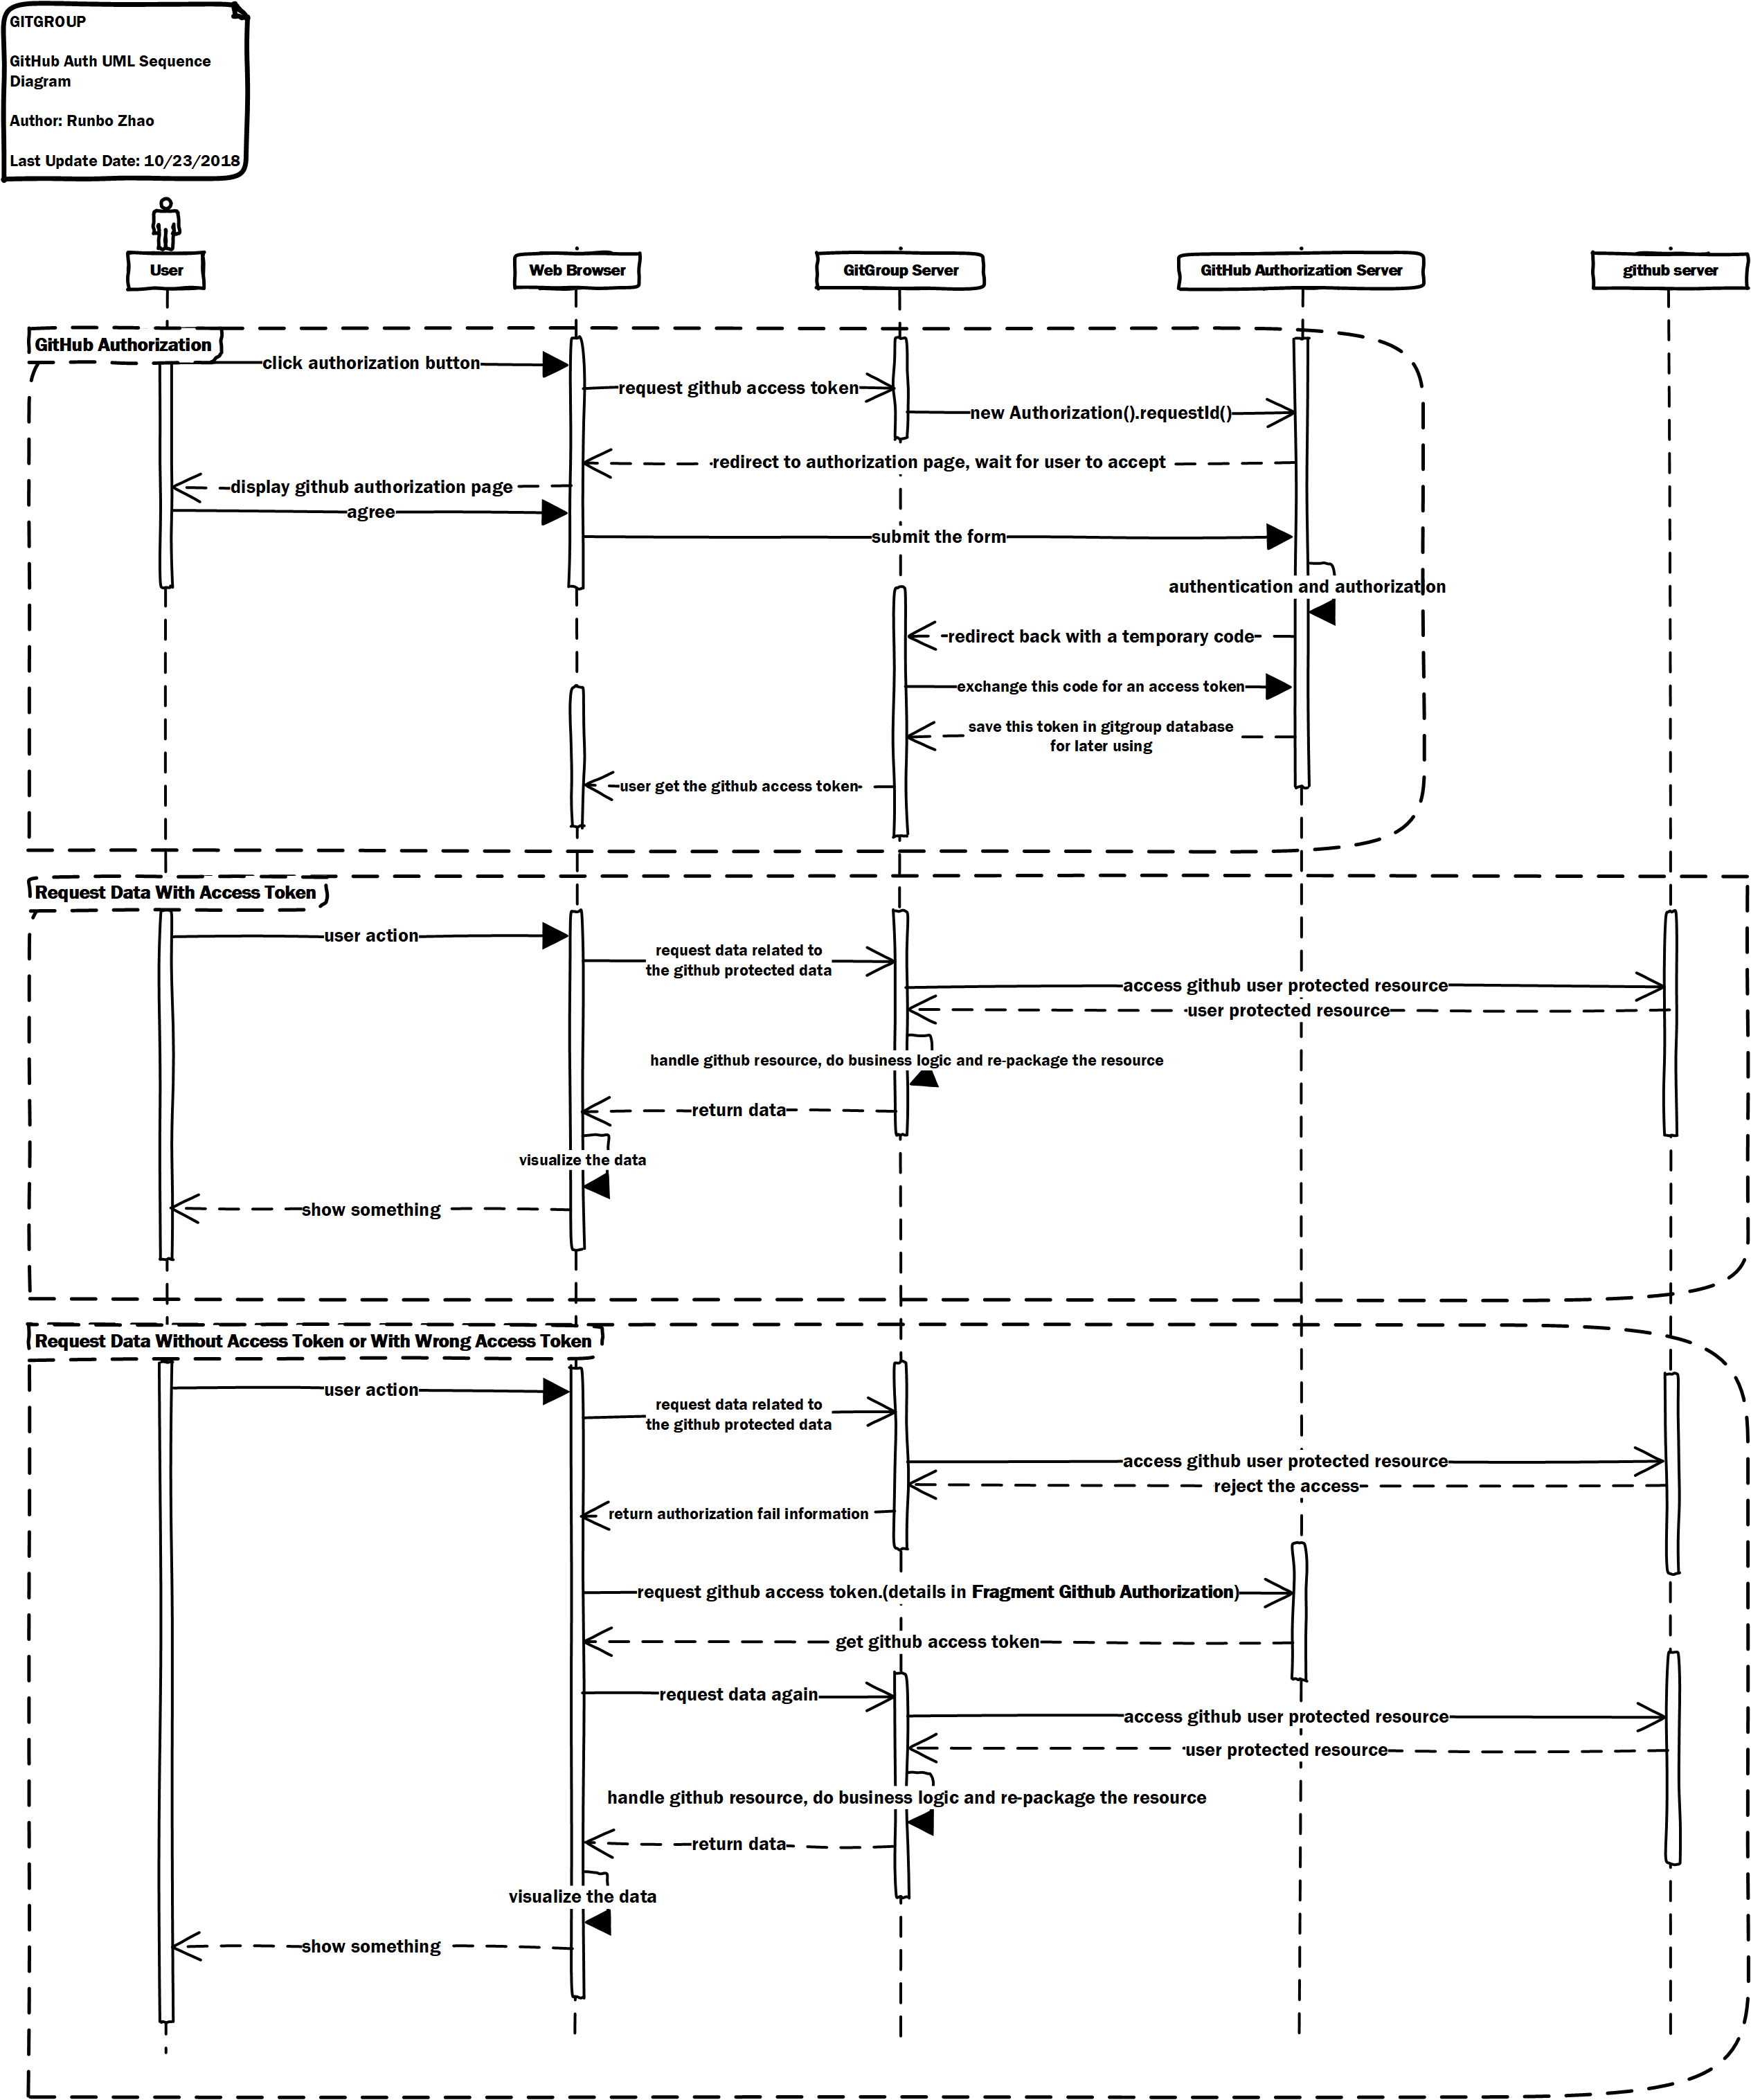
\includegraphics[width=\textwidth]{./pics/AuthSequenceDiagram.png}
	\caption{\textbf{DETAIL} Sequence Diagram For Authorization}
\end{figure}

\begin{figure}[h]
	\centering
	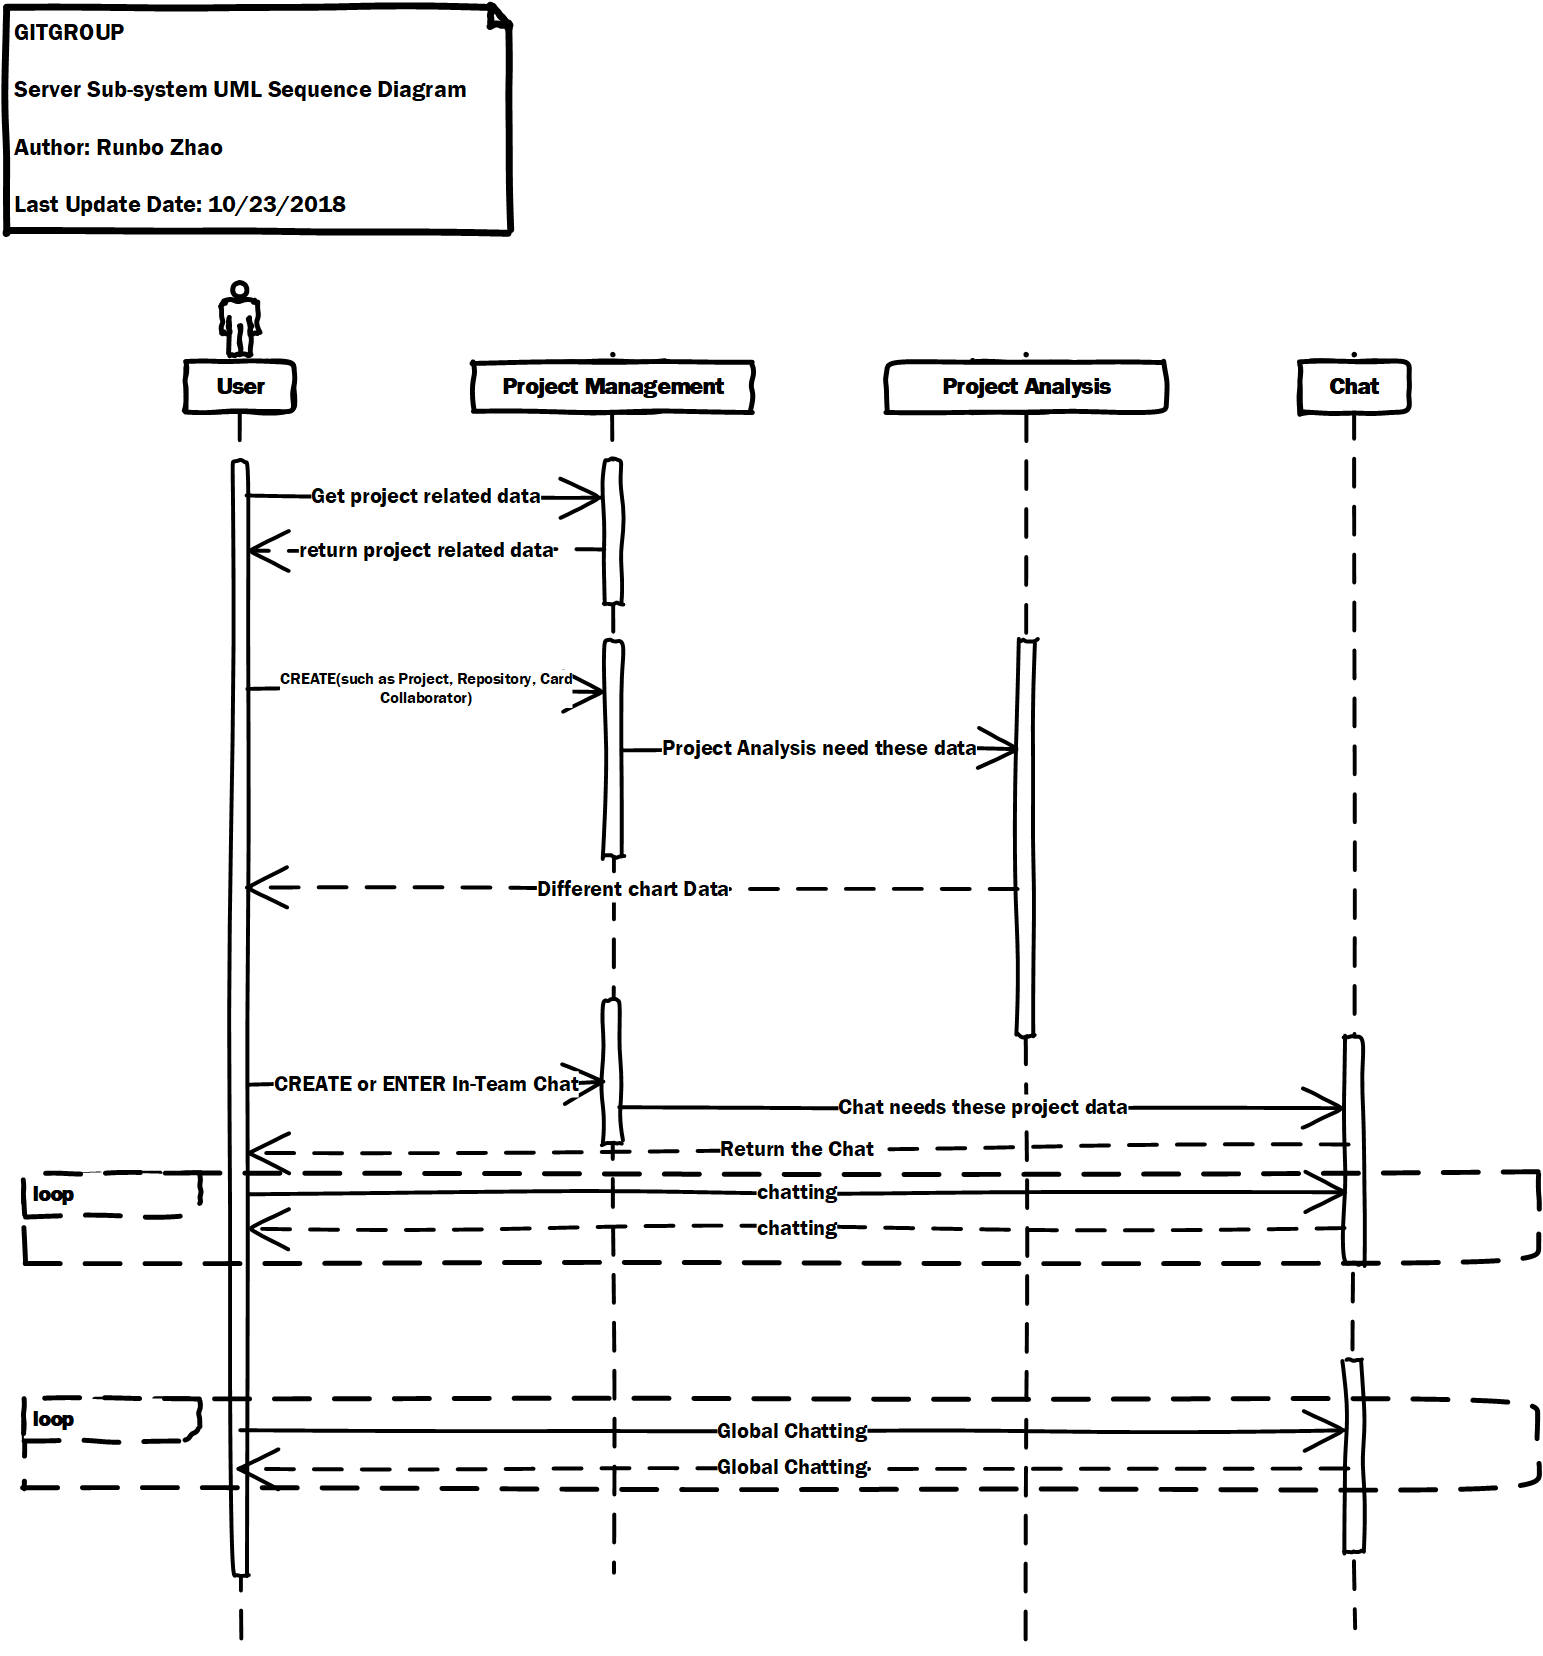
\includegraphics[width=\textwidth]{./pics/SubSysSequenceDiagram.png}
	\caption{\textbf{DETAIL} Sequence Diagram For Sub-Systems}
\end{figure}

\begin{figure}[h]
	\centering
	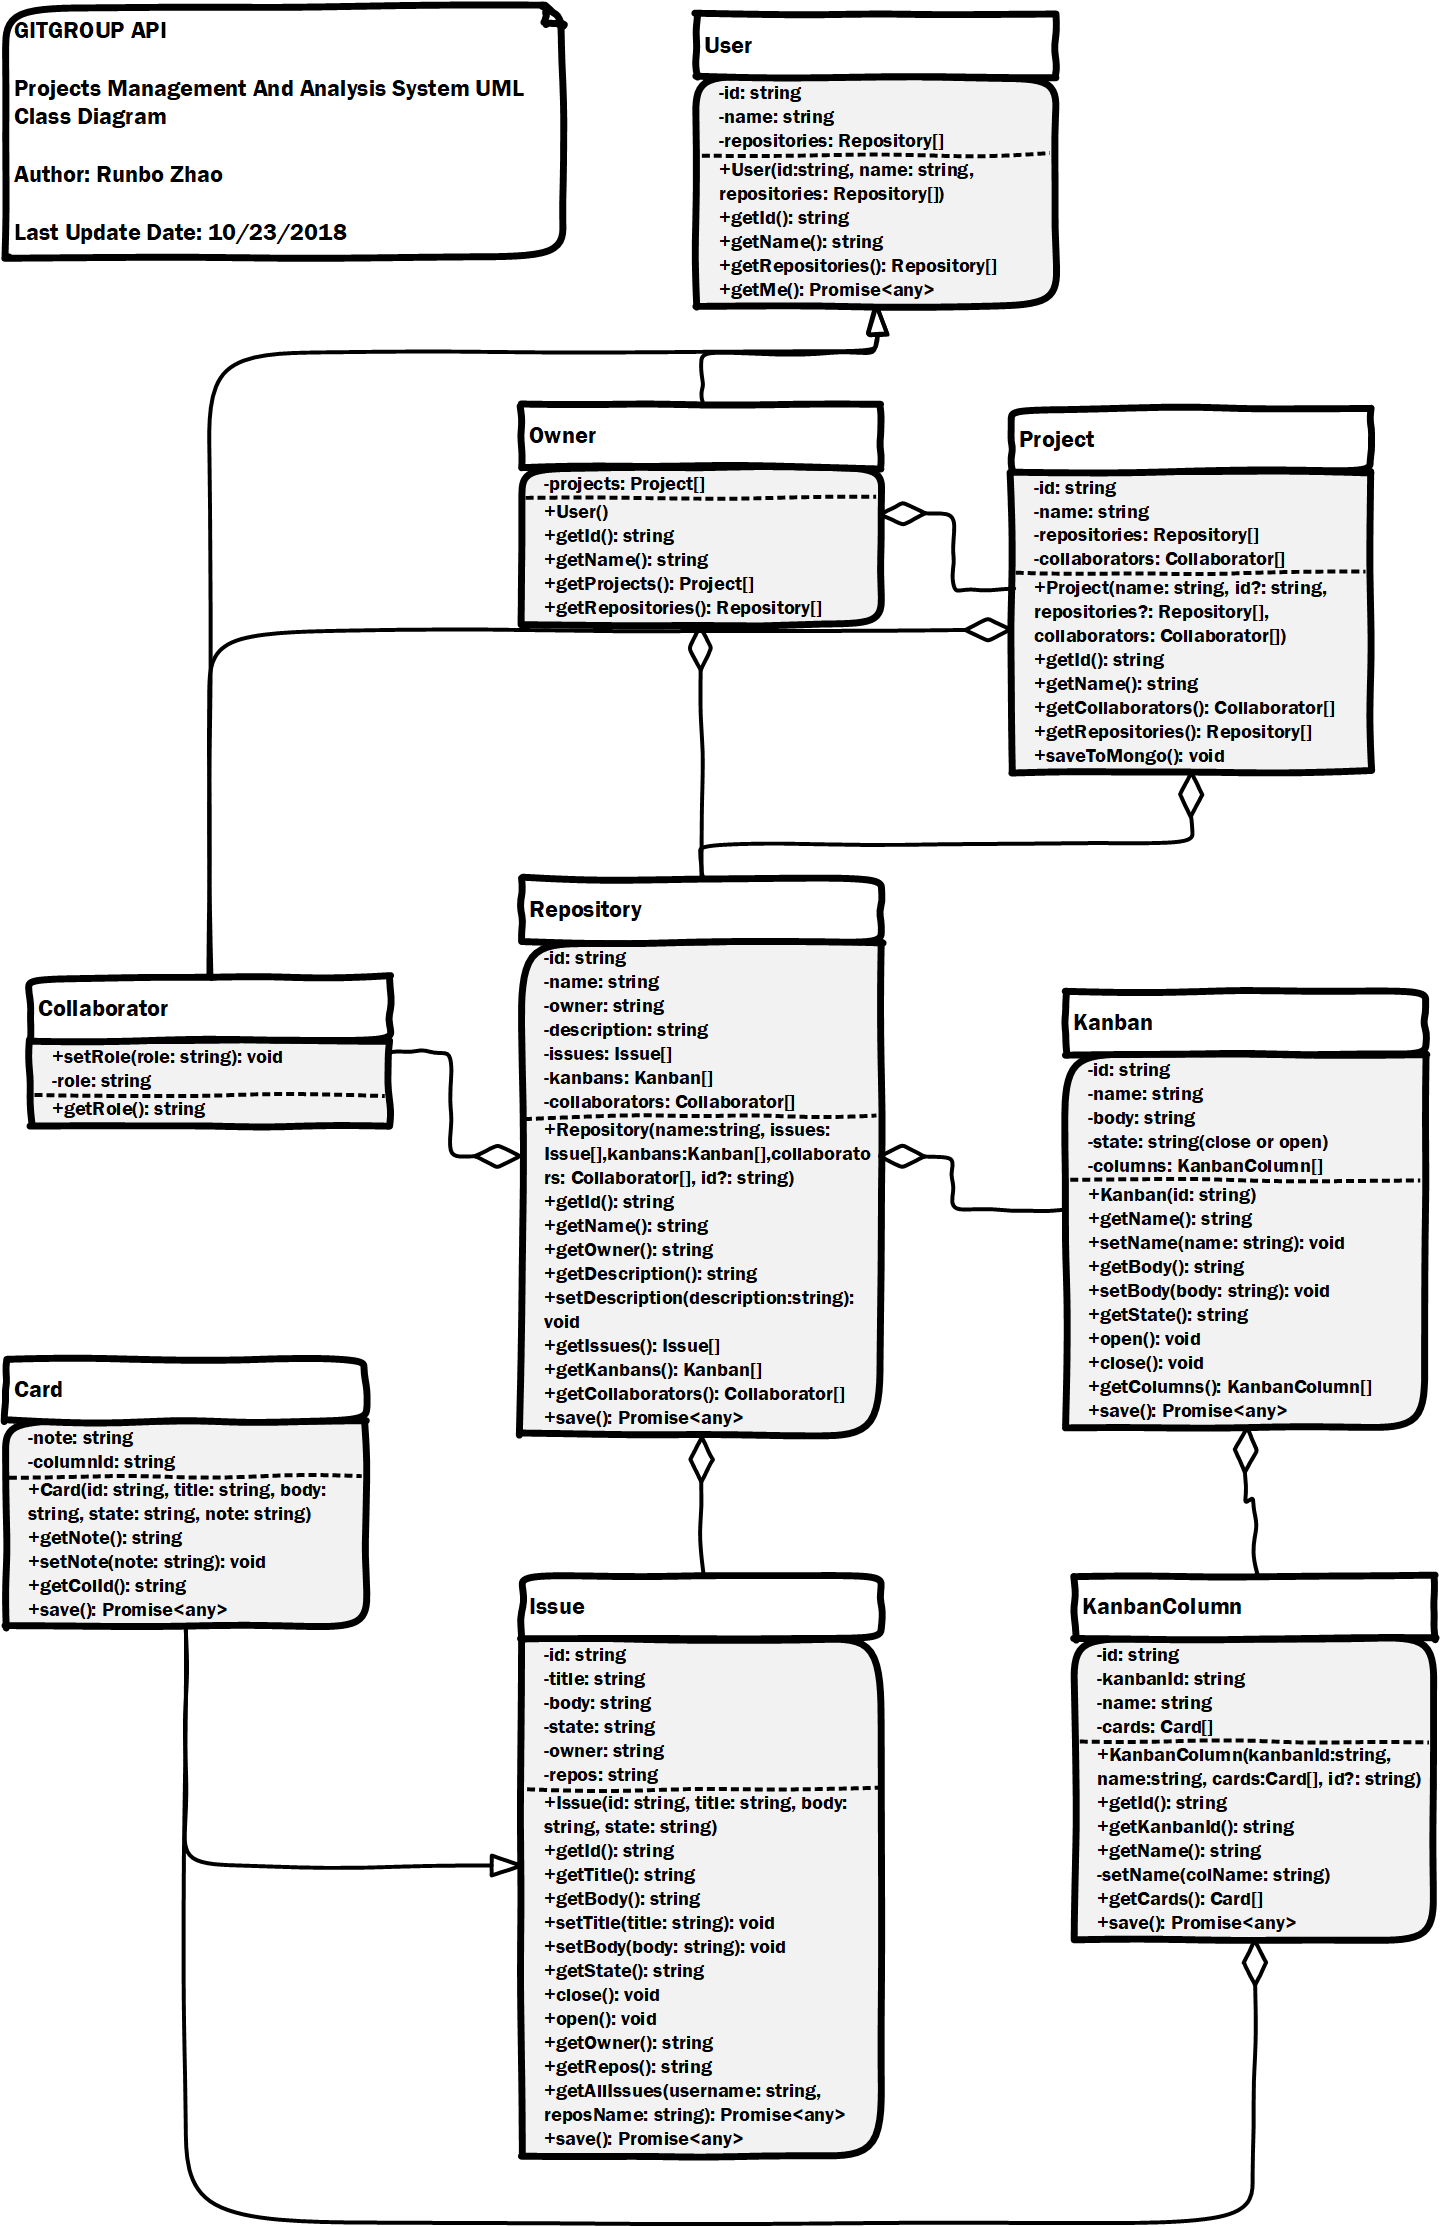
\includegraphics[height=0.95\textheight]{./pics/ClassDiagram.png}
	\caption{\textbf{DETAIL} UML Class Diagram}
\end{figure}


\cleardoublepage
\listoffigures
\cleardoublepage
\listoftables

% -------------------------------------------------------
% References
% -------------------------------------------------------
\bibliographystyle{apacite}
\bibliography{References}



\end{document}